\documentclass[11pt,a4paper,oneside]{report}
\usepackage[T1]{fontenc}
\usepackage[utf8]{inputenc}
\usepackage[italian]{babel}
\usepackage{amsmath,amssymb}
\usepackage{mathtools}
\usepackage{siunitx}
\usepackage{graphicx}
\usepackage{booktabs}
\usepackage{longtable}
\usepackage{array}
\usepackage{geometry}
\usepackage{hyperref}
\usepackage{xcolor}
\usepackage{float}
\usepackage{tikz}
\usepackage{listings}
\lstset{language=Matlab,basicstyle=\ttfamily\footnotesize,
  columns=fullflexible,keepspaces=true,breaklines=true,
  showstringspaces=false,tabsize=2,frame=single,
  rulecolor=\color{black!20},commentstyle=\color{black!60},
  keywordstyle=\color{blue!45!black},aboveskip=.7em,belowskip=.7em}
\usepackage[protrusion=true,expansion=false]{microtype}
\geometry{top=2.5cm,bottom=2.5cm,left=2.7cm,right=2.3cm}
\hypersetup{hypertexnames=false,colorlinks=true,linkcolor=blue!45!black,urlcolor=blue!55!black,pdftitle={Controllo robusto di un manipolatore planare 2-DoF con SEA},pdfauthor={Alessio de Dato; Valerio Rebechi}}
\setlength{\emergencystretch}{3em}
\setlength{\parindent}{1.2em}
\renewcommand{\arraystretch}{1.12}
\newcommand{\status}[1]{\texttt{#1}}
\newcommand{\artifact}[1]{\texttt{#1}}
% Generated by build_m18_report_values.m. Do not edit.
\newcommand{\MOneMass}{1}
\newcommand{\MTwoMass}{0.8}
\newcommand{\LOneLength}{0.4}
\newcommand{\LTwoLength}{0.3}
\newcommand{\JmOne}{0.01}
\newcommand{\BmOne}{0.02}
\newcommand{\KOne}{50}
\newcommand{\KTwo}{40}
\newcommand{\GravityValue}{9.81}
\newcommand{\EquilibriumQOneDeg}{90}
\newcommand{\EquilibriumQTwoDeg}{0}
\newcommand{\OpenLoopMaxRealPole}{7.20943}
\newcommand{\ActuatorWn}{40}
\newcommand{\ActuatorZeta}{0.8}
\newcommand{\ActuatorDelayMs}{15}
\newcommand{\FullPlantOrder}{14}
\newcommand{\JmOneUncertaintyPct}{9}
\newcommand{\KOneUncertaintyPct}{7}
\newcommand{\KTwoUncertaintyPct}{7}
\newcommand{\MFourBlockCount}{5}
\newcommand{\SettlingTarget}{0.8}
\newcommand{\OvershootTarget}{10}
\newcommand{\ErrorTargetPct}{5}
\newcommand{\CrossTargetPct}{25}
\newcommand{\PerformanceBandwidth}{12}
\newcommand{\UScaleNm}{12}
\newcommand{\MControllerOrder}{14}
\newcommand{\MControllerWorstTs}{0.776}
\newcommand{\MSevenStatus}{PARTIAL}
\newcommand{\MSevenAdmissible}{0}
\newcommand{\MControllerRasMin}{60}
\newcommand{\MixsynGamma}{10.2071}
\newcommand{\HinfsynGamma}{10.2071}
\newcommand{\KhinfOrder}{18}
\newcommand{\AFiveGamma}{10.2477}
\newcommand{\AFiveRSLower}{0.875899}
\newcommand{\AFiveRSUpper}{0.882789}
\newcommand{\MusynObjective}{10.4032}
\newcommand{\BestDKIteration}{3}
\newcommand{\KmuOrder}{52}
\newcommand{\KmuNPStatus}{FAIL}
\newcommand{\KmuRSStatus}{PASS\_CERTIFIED}
\newcommand{\KmuRPStatus}{FAIL\_CERTIFIED}
\newcommand{\KmuRSLower}{1.25004}
\newcommand{\KmuRSUpper}{1.25257}
\newcommand{\KhinfRasMin}{52.8763}
\newcommand{\KmuRasMin}{60}
\newcommand{\MonteCarloSeed}{20260826}
\newcommand{\MonteCarloSamples}{40}
\newcommand{\MControllerStableSamples}{39}
\newcommand{\KhinfStableSamples}{40}
\newcommand{\KmuStableSamples}{40}
\newcommand{\MControllerSampleFivePole}{1.80447}
\newcommand{\MControllerTrackingPassPct}{30}
\newcommand{\KhinfTrackingPassPct}{0}
\newcommand{\KmuTrackingPassPct}{0}
\newcommand{\FinalRobustController}{Kmu}
\newcommand{\NominalReferenceController}{M6}
\newcommand{\HinfReferenceController}{Khinf}

\newcommand{\RevQs}{\num{0.08726646}}
\newcommand{\RevQds}{\num{1.047198}}
\newcommand{\RevDeltaScale}{\num{0.0125}}
\newcommand{\RevCareResidual}{\num{2.912849e-10}}
\newcommand{\RevRegulatorDecay}{\num{6.171691}}
\newcommand{\RevEstimatorDecay}{\num{9.31874}}
\newcommand{\RevSeparation}{\num{2.094409e-13}}
\newcommand{\RevRn}{\num{7.615435e-07}}
\newcommand{\RevCubicBound}{\num{18893}}
\newcommand{\RevHinfCrossover}{\num{13.83908}}
\newcommand{\RevTrajectoryFinalV}{\num{7.155528e-07}}
\newcommand{\RevTrajectoryIncrement}{\num{7.369284e-22}}

% Source: MATLAB export_hinf_final_results, summary.json
\newcommand{\FinalGamma}{0.0474606}
\newcommand{\FinalOrder}{22}
\newcommand{\FinalMuGamma}{0.63468}
\newcommand{\FinalMuOrder}{78}
\newcommand{\FinalMuObjective}{0.88381}
\newcommand{\FinalMinOrder}{2}
\newcommand{\FinalHRSLowerBound}{0.0181249}
\newcommand{\FinalHRSUpperBound}{0.0181617}
\newcommand{\FinalHRPLowerBound}{0.0172543}
\newcommand{\FinalHRPUpperBound}{0.0171945}
\newcommand{\FinalMuRSLowerBound}{1.7998}
\newcommand{\FinalMuRSUpperBound}{1.80442}
\newcommand{\FinalMuRPLowerBound}{1.67717}
\newcommand{\FinalMuRPUpperBound}{1.68066}

\newcommand{\NoiseHinfPeak}{\ensuremath{4.93\times10^{5}}}
\newcommand{\NoiseHinfRms}{\ensuremath{1.32\times10^{4}}}
\newcommand{\NoiseMuPeak}{87.1}
\newcommand{\NoiseMuRms}{8.29}

\newcommand{\SimHinfNLPeak}{\ensuremath{7.33\times10^{5}}}
\newcommand{\SimMuLinPeak}{108}
\renewcommand{\FinalHRSLowerBound}{0.0261539}
\renewcommand{\FinalHRSUpperBound}{0.0262069}
\renewcommand{\FinalHRPLowerBound}{0.0306781}
\renewcommand{\FinalHRPUpperBound}{0.0301044}
\renewcommand{\FinalMuRSLowerBound}{1.7998}
\renewcommand{\FinalMuRSUpperBound}{1.80442}
\renewcommand{\FinalMuRPLowerBound}{1.67717}
\renewcommand{\FinalMuRPUpperBound}{1.68066}
\newcommand{\FinalHRSFrequency}{62.24}

\title{Controllo robusto di un manipolatore planare 2-DoF con Series Elastic Actuators}
\author{Alessio de Dato \\ \small Matricola 635256 \\[0.8em]
Valerio Rebechi \\ \small Matricola 722224}
\date{01.11.2026}
\begin{document}
\hypersetup{pageanchor=false}
\maketitle
\hypersetup{pageanchor=true}
\pagenumbering{roman}
\begin{abstract}
Si conserva il progetto del manipolatore planare SEA a due giunti, dalle
equazioni non lineari alla linearizzazione a 14 stati, concentrando lo
studio sulle incertezze dei due attuatori SISO. La stessa famiglia fisica,
con frequenza naturale e smorzamento indipendenti nei due canali, viene
descritta mediante parametri reali e mediante un peso dinamico concentrato.
Il confronto segue il procedimento del corso: campionamento, scostamenti,
inviluppo, fitting, perturbazioni normalizzate e LFT.
LQG, LQGI, sensibilita mista, controllo a due gradi di liberta, PID
strutturato e D--K rimangono strumenti per interpretare gli effetti
dell'incertezza. Si distinguono analisi a controllore fissato e sintesi
dedicate, verificandole sugli stessi dieci impianti fisici.
I margini robusti non sostituiscono i target temporali e non risolvono
l'amplificazione del rumore: i picchi fra campioni sono analizzati
esplicitamente. Le sezioni empiriche RAS usano quindici condizioni iniziali,
separando convergenza, mancata convergenza e limiti numerici.
I risultati storici M4 sono conservati e identificati; nessuna garanzia
viene trasferita al nuovo insieme senza una nuova analisi. Il percorso
operativo accorpa i sorgenti esistenti e genera una consegna autonoma.
\end{abstract}
\tableofcontents
\listoffigures
\listoftables
\clearpage
\pagenumbering{arabic}
\chapter{Introduzione e obiettivi}
\section{Problema fisico}
Un manipolatore con attuatori elastici in serie non trasmette rigidamente il moto dei motori ai link. Fra ciascun rotore e il braccio si trova una molla torsionale: il motore deve deformarla per produrre la coppia sul giunto. Questa elasticità rende il comportamento più ricco di quello di un manipolatore rigido e introduce oscillazioni che il controllo deve smorzare.

Studiamo il manipolatore planare a due giunti assegnato nella traccia del corso. All'estremità del secondo link consideriamo anche una massa aggiuntiva, che rappresenta il carico dell'end-effector. Il suo valore può cambiare durante l'impiego del robot. Anche i due drive sono conosciuti solo approssimativamente: frequenza naturale, smorzamento e ritardo possono discostarsi dai valori nominali.

Il punto centrale del lavoro è confrontare due modi di descrivere queste incertezze. Nel modello A manteniamo espliciti i parametri fisici dei drive; nel modello B raccogliamo le loro variazioni in due perturbazioni dinamiche pesate. La massa del carico rimane invece un parametro reale in entrambi. In questo modo il confronto riguarda due descrizioni degli stessi attuatori e della stessa meccanica.

\section{Obiettivi di controllo}
Vogliamo stabilizzare il braccio nella configurazione verticale superiore, seguire piccoli riferimenti articolari e limitare gli effetti di coppie disturbanti applicate ai link. Confrontiamo LQG, LQGI, controllo $H_\infty$ a uno e due gradi di libertà, PID strutturato e sintesi robusta mediante iterazione D--K.

Queste strategie rispondono a domande diverse. LQG bilancia stato e comando e ricostruisce gli stati non misurati; l'integratore corregge gli errori persistenti. La sintesi $H_\infty$ limita una norma pesata, mentre la sintesi con $\mu$ tiene conto della struttura delle incertezze. Per valutarle usiamo gli stessi riferimenti, disturbi e impianti fisici campionati.

\section{Metodo di lavoro e classi di verifica}
Distinguiamo quattro proprietà. La stabilità nominale, NS, riguarda la convergenza degli stati nel modello nominale. La prestazione nominale, NP, richiede anche che una mappa pesata abbia norma minore di uno. La stabilità robusta, RS, estende la stabilità a tutta la famiglia ammessa. La prestazione robusta, RP, richiede stabilità e limite prestazionale per tutti i suoi elementi.

Queste definizioni non sostituiscono le prove temporali. Un controllore può soddisfare una norma pesata e avere un transitorio poco adatto, oppure amplificare il rumore fino a richiedere coppie irragionevoli. Per questo affianchiamo all'analisi robusta tracking, disturbi, sforzo di controllo e simulazioni non lineari. I campioni danno evidenza numerica; non dimostrano da soli una proprietà sull'intero insieme.

\section{Organizzazione della relazione}
Partiamo dalle equazioni fisiche, dall'equilibrio e dalla linearizzazione. Introduciamo poi i drive e le due rappresentazioni delle incertezze. Dopo aver definito obiettivi e pesi, progettiamo i controllori e ne discutiamo la robustezza. Le simulazioni non lineari, la regione di attrazione empirica e i dieci impianti comuni permettono infine di interpretare vantaggi e limiti delle soluzioni. Le appendici raccolgono parametri, istruzioni di riproduzione e pochi estratti MATLAB essenziali.

\chapter{Modello dinamico del manipolatore SEA}
\section{Coordinate e struttura meccanica}
Il manipolatore è costituito da due link planari con giunti rotoidali. La coordinata $q_1$ individua l'orientamento del primo link, mentre $q_2$ è relativa al primo e determina quindi l'orientamento assoluto del secondo attraverso $q_1+q_2$. Le masse sono concentrate secondo il modello fornito dalla traccia. La matrice di inerzia dipende da $q_2$, perciò il movimento di un giunto modifica l'energia cinetica associata all'altro.

Ogni giunto è azionato da un motore con inerzia $J_{mi}$ e smorzamento viscoso $B_{mi}$. Fra rotore e link è interposta una molla torsionale di rigidezza $k_i$. Definiamo
\[
\delta=\theta-q,\qquad \tau_{el}=K_s\delta,\qquad
K_s=\operatorname{diag}(k_1,k_2).
\]
Il segno di $\delta$ è scelto in modo che una coordinata motore maggiore della corrispondente coordinata link produca una coppia positiva sul link. La stessa coppia compare con segno opposto nell'equazione del motore, rispettando il principio di azione e reazione.

\section{Equazioni del lato link e del lato motore}
La dinamica assegnata si scrive
\begin{align}
M(q)\ddot q+C(q,\dot q)\dot q+G(q)&=K_s(\theta-q),\\
J_m\ddot\theta+B_m\dot\theta&=\tau-K_s(\theta-q).
\end{align}
La prima equazione raccoglie inerzia, termini di Coriolis e centrifughi e gravità del braccio. La seconda descrive la dinamica dei rotori: la coppia comandata $\tau=[\tau_1,\tau_2]^T$ viene impiegata sia per accelerare i motori sia per deformare le molle. Non viene introdotto uno smorzamento viscoso lato link perché non compare nella traccia; $B_m$ agisce esclusivamente sulle velocità dei rotori.

La matrice di inerzia è
\[
M(q)=\begin{bmatrix}
(m_1+m_2)l_1^2+m_2l_2^2+2m_2l_1l_2\cos q_2&m_2l_2^2+m_2l_1l_2\cos q_2\\
m_2l_2^2+m_2l_1l_2\cos q_2&m_2l_2^2
\end{bmatrix}.
\]
La simmetria di $M(q)$ deriva dall'energia cinetica. Per parametri fisici positivi il determinante si riduce a
\[
\det M(q)=m_2l_1^2l_2^2\left(m_1+m_2\sin^2 q_2\right)>0,
\]
e $m_{11}$ è positivo; il criterio di Sylvester garantisce pertanto che $M(q)$ sia definita positiva per ogni configurazione. Questa proprietà consente di ottenere le accelerazioni risolvendo sistemi lineari, senza ricorrere all'inversa esplicita.

Con $h=m_2l_1l_2\sin q_2$, i termini rimanenti sono
\[
C(q,\dot q)=\begin{bmatrix}-h\dot q_2&-h(\dot q_1+\dot q_2)\\h\dot q_1&0\end{bmatrix},\quad
G(q)=\begin{bmatrix}(m_1+m_2)gl_1\cos q_1+m_2gl_2\cos(q_1+q_2)\\m_2gl_2\cos(q_1+q_2)\end{bmatrix}.
\]
La struttura di $C$ è coerente con la proprietà di passività del manipolatore: la parte simmetrica di $\dot M-2C$ è nulla. Il vettore $G(q)$ usa la convenzione angolare della traccia, nella quale i contributi gravitazionali sono proporzionali ai coseni degli angoli assoluti dei link.

\section{Stato, ingressi e uscite}
Lo stato meccanico a otto componenti è ordinato come
\[
x=\begin{bmatrix}q^T&\dot q^T&\theta^T&\dot\theta^T\end{bmatrix}^T.
\]
Con questa convenzione le equazioni del primo ordine sono
\begin{align}
\dot q&=\dot q,\\
\ddot q&=M(q)\backslash\left[K_s(\theta-q)-C(q,\dot q)\dot q-G(q)\right],\\
\dot\theta&=\dot\theta,\\
\ddot\theta&=J_m\backslash\left[\tau-B_m\dot\theta-K_s(\theta-q)\right].
\end{align}
L'uscita primaria di prestazione è $q$, perché la consegna richiede la regolazione delle articolazioni. Per l'osservatore sono disponibili le quattro posizioni $[q^T,\theta^T]^T$, ottenibili con encoder lato link e lato motore; non assumiamo misure dirette delle velocità. La disponibilità di entrambe le posizioni consente inoltre di ricavare direttamente la deformazione elastica.

\section{Implementazione e verifiche}
Abbiamo separato inerzia, Coriolis, gravità, coppia elastica ed equazioni differenziali in funzioni numeriche indipendenti. Questa scomposizione permette di verificare le proprietà fisiche prima di utilizzare il modello nelle sintesi. I parametri nominali sono centralizzati e riportati nell'Appendice~\ref{app:parametri}.

La validazione ha controllato la simmetria e la positività di $M(q)$ su 2001 configurazioni, la proprietà di skew-symmetry associata a $\dot M-2C$, le formule di gravità e coppia elastica e la finitezza del campo vettoriale. Il minimo autovalore di $M$ osservato è $0.01904$ kg m$^2$ e il massimo residuo della proprietà energetica è dell'ordine di $10^{-18}$. Il campionamento numerico non sostituisce la dimostrazione analitica di positività, ma verifica che l'implementazione rispetti le equazioni.

\section{Assunzioni e limiti del modello}
Il modello meccanico non include attrito secco, giochi, flessibilità distribuita dei link, backlash, saturazioni o limiti di corsa. Le molle sono lineari e le inerzie dei motori sono riferite direttamente alle coordinate $\theta$. Queste semplificazioni sono coerenti con la traccia e rendono interpretabile il confronto fra controllori; i loro effetti devono però essere ricordati quando si interpretano le simulazioni non lineari e i margini robusti.

\chapter{Equilibrio e linearizzazione}
\section{Scelta del punto di lavoro}
Scegliamo il braccio disteso nella configurazione verticale superiore:
\[
 \bar q=[\pi/2,0]^T,\qquad \dot{\bar q}=\dot{\bar\theta}=0.
\]
È un punto interessante perché la gravità lo rende instabile in anello aperto. Il controllo deve quindi stabilizzarlo, oltre a inseguire il riferimento.

Dalle equazioni statiche ricaviamo
\[
 \bar\tau=G(\bar q),\qquad \bar\theta=\bar q+K_s^{-1}G(\bar q).
\]
Qui entrambi i coseni di $G$ sono nulli: coppia e deformazione d'equilibrio sono nulle per ogni $m_2\in[0.72,0.88]$ kg. La massa del secondo link non sposta quindi questo particolare punto di lavoro. La linearizzazione cambia ugualmente, perché la pendenza della gravità e l'inerzia dipendono da $m_2$. Un pendolo verticale può avere coppia gravitazionale nulla esattamente in alto e una forza destabilizzante diversa appena si sposta: è questa pendenza che entra nel Jacobiano.

Il residuo della dinamica non lineare all'equilibrio è \FinResiduoEquilibrio, inferiore alla tolleranza $10^{-10}$. Le quantità molto piccole sono residui del calcolo in doppia precisione.

Le due relazioni statiche hanno un significato distinto: la molla
sostiene la gravità del link, il motore equilibra la reazione della molla.
Qui $G(\bar q)=0$, ma la configurazione rimane instabile: essere in
equilibrio significa avere derivata nulla esattamente nel punto,
non ritornarvi dopo un piccolo spostamento.

\section{Coordinate incrementali e Jacobiani}
Introduciamo $\widetilde x_m=x_m-\bar x_m$ e
$\widetilde\tau=\tau-\bar\tau$. Lo sviluppo al primo ordine dà
\[
 \dot{\widetilde x}_m=A_m\widetilde x_m+B_\tau\widetilde\tau+B_dd,
 \quad A_m=\left.\frac{\partial f}{\partial x_m}\right|_{\bar x_m},
 \quad B_\tau=\left.\frac{\partial f}{\partial\tau}\right|_{\bar x_m}.
\]
Il termine costante è nullo perché abbiamo verificato l'equilibrio.
Le derivate descrivono la risposta a piccoli spostamenti, non a un
moto arbitrariamente ampio. La massa continua a comparire in queste
derivate anche quando il valore della gravità nel punto è zero.

Poniamo $\widetilde x_m=x_m-\bar x_m$ e $\widetilde\tau=\tau-\bar\tau$. Definendo $\bar M=M(\bar q)$ e $K_g=\partial G/\partial q|_{\bar q}$, otteniamo
\[
 A_m=\begin{bmatrix}
 0&I&0&0\\
 -\bar M^{-1}(K_s+K_g)&0&\bar M^{-1}K_s&0\\
 0&0&0&I\\
 J_m^{-1}K_s&0&-J_m^{-1}K_s&-J_m^{-1}B_m
 \end{bmatrix},
\quad B_\tau=\begin{bmatrix}0\\0\\0\\J_m^{-1}\end{bmatrix},
\quad B_d=\begin{bmatrix}0\\\bar M^{-1}\\0\\0\end{bmatrix}.
\]
I blocchi sono di dimensione $2\times2$. Il termine $C\dot q$ è quadratico nelle velocità e non contribuisce al Jacobiano in un equilibrio statico. La sua dipendenza dal carico rimane invece nella simulazione non lineare.

Per la massa $m_2$ nominale si ha
\[
 \bar M=\begin{bmatrix}0.552&0.168\\0.168&0.072\end{bmatrix}\ \mathrm{kg\,m^2},\qquad
 K_g=\begin{bmatrix}-9.4176&-2.3544\\-2.3544&-2.3544\end{bmatrix}\ \mathrm{N\,m/rad}.
\]
Mostriamo quattro decimali in $K_g$ per rendere controllabile il calcolo; le altre matrici complete restano nei dati MATLAB. Il confronto con differenze finite centrate dà un errore relativo \FinErroreJacobiano. La stessa verifica viene eseguita anche ai due estremi di $m_2$.

Il confronto a differenze finite usa le stesse equazioni fisiche e
una costruzione indipendente del Jacobiano. Un accordo numerico
controlla l'implementazione della linearizzazione; non misura da solo
il raggio entro cui l'approssimazione è sufficientemente accurata.
Il resto di Taylor tende a zero più rapidamente del termine lineare
al diminuire dell'ampiezza, ma il comportamento a grande spostamento
va valutato sulle equazioni complete.

\section{Poli e proprietà strutturali}
Il modello meccanico ha otto stati e due poli reali instabili, riportati nella Tabella~\ref{tab:poli}. Le oscillazioni elastiche hanno frequenze più alte e richiedono di evitare un controllo troppo aggressivo.

\begin{table}[htbp]\centering\small
\setlength{\tabcolsep}{4pt}
\begin{tabular}{lr}\toprule
Poli meccanici [s$^{-1}$] & Esito\\\midrule
\num{7.209} & instabile\\
\num{4.041} & instabile\\
\num{-0.6838} $\pm j$ \num{79.4} & stabile\\
\num{-0.9619} $\pm j$ \num{69.95} & stabile\\
\num{-4.073} & stabile\\
\num{-7.886} & stabile\\
\bottomrule\end{tabular}
\caption{Poli degli otto stati meccanici al carico nominale; le righe complesse rappresentano coppie coniugate.}
\label{tab:poli}
\end{table}


\begin{figure}[!htbp]\centering
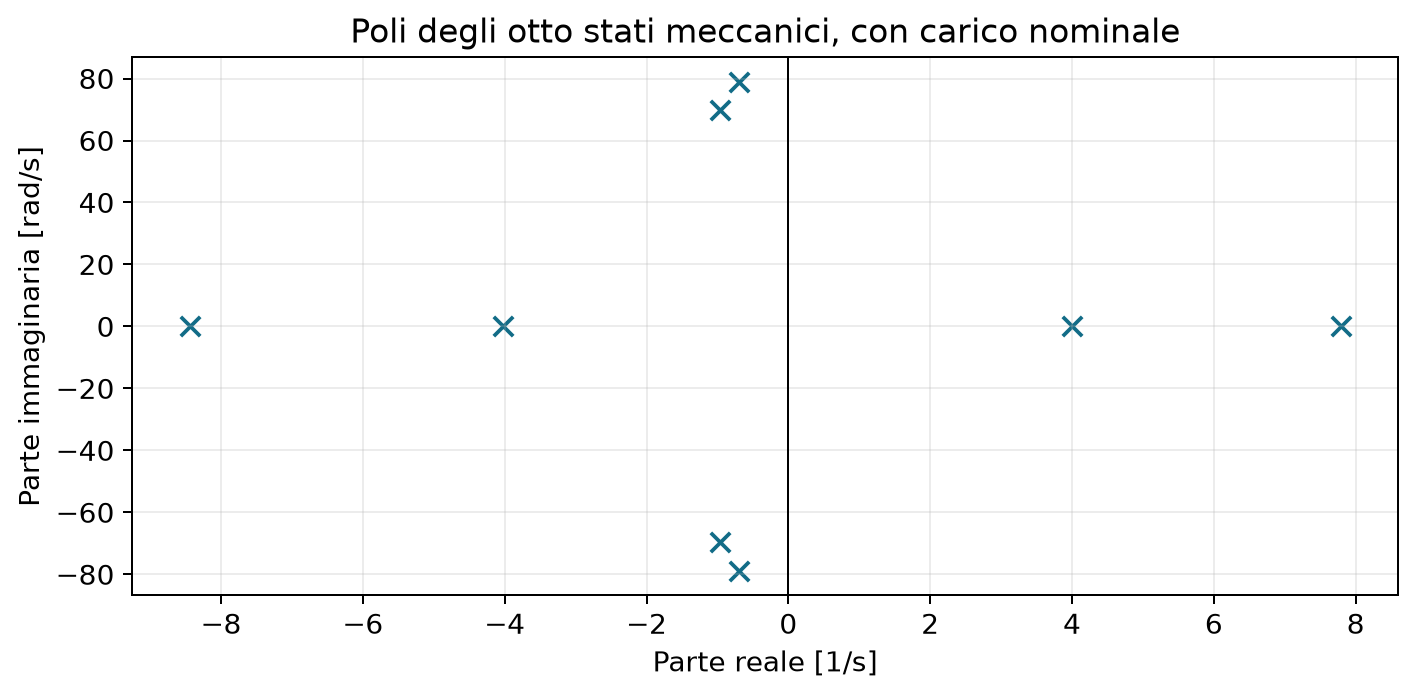
\includegraphics[width=.85\linewidth]{figures/editoriale/poli_meccanici.png}
\caption{Spettro della matrice meccanica salvata con massa nominale.
I poli reali positivi indicano l'instabilità della postura; le coppie
complesse distinguono i modi elastici più rapidi. È una visualizzazione
della linearizzazione disponibile, ricalcolata sul modello corrente.}
\end{figure}

Usiamo il criterio PBH su tutti i modi per verificare che le coppie possano controllarli e che gli encoder possano osservarli. Il modello completo è controllabile e osservabile: i ranghi PBH sono entrambi 14. In particolare è stabilizzabile e rilevabile. Questo è il controllo strutturale necessario alle sintesi; non ricaviamo conclusioni dal solo rango di matrici contenenti alte potenze di $A_m$.

La linearizzazione descrive piccole variazioni attorno all'equilibrio. Per spostamenti maggiori valutiamo direttamente le equazioni non lineari. La stabilità del modello lineare non viene presentata come una garanzia globale sul braccio.

Il criterio PBH controlla se un modo instabile può essere influenzato
dalle coppie e ricostruito dalle misure. Le matrici classiche di
controllabilità e osservabilità contengono alte potenze di $A_m$:
con scale meccaniche e attuative diverse possono essere mal condizionate.
Per le sintesi servono stabilizzabilità e rilevabilità dei modi critici,
non un rango dichiarato senza tolleranza numerica.
Le frequenze elastiche più elevate spiegano inoltre perché aumentare
molto la rapidità del feedback possa richiedere più coppia e rendere
più rilevante l'incertezza dei drive.


\chapter{Attuatori e pianta completa}
\section{Modello nominale}
La coppia richiesta dal controllore non viene applicata direttamente alla dinamica SEA. Per rappresentare banda finita e latenza, ogni canale è descritto da un secondo ordine a guadagno statico unitario seguito da un ritardo di trasporto:
\[
\bar G_m(s)=\frac{\bar\omega_n^2}{s^2+2\bar\zeta\bar\omega_n s+\bar\omega_n^2}e^{-\bar\tau_ds},
\]
con $\bar\omega_n=\ActuatorWn$ rad/s, $\bar\zeta=\ActuatorZeta$ e $\bar\tau_d=\ActuatorDelayMs$ ms. Questi valori non sono dati identificati: sono stati selezionati fra 27 combinazioni di frequenza naturale, smorzamento e ritardo. I criteri richiedono una banda sensibilmente maggiore dei modi instabili a bassa frequenza, ma inferiore ai primi modi elastici; impongono inoltre overshoot del singolo attuatore non superiore al 2\% e un errore di fase Padé moderato a 80 rad/s.

La combinazione scelta, $40$ rad/s, $0.8$ e $15$ ms, fornisce una banda di circa $34.78$ rad/s. È quindi abbastanza rapida rispetto ai poli instabili a 4.04 e 7.21 s$^{-1}$, mentre inizia a filtrare il comando prima delle risonanze elastiche a circa 70--79 rad/s. Lo smorzamento $0.8$ limita la sovraelongazione senza imporre una dinamica criticamente smorzata; il ritardo di 15 ms rimane non trascurabile e viene incluso esplicitamente.

\section{Approssimazione del ritardo}
La traccia richiede un Padé del primo ordine:
\[
e^{-\tau_ds}\simeq \frac{1-\tau_ds/2}{1+\tau_ds/2}.
\]
L'approssimazione aggiunge un polo stabile in $-2/\tau_d$ e uno zero nel semipiano destro in $+2/\tau_d$. Lo zero è conseguenza della rappresentazione razionale del ritardo e rende il canale non minimum-phase, ma non introduce un polo instabile. L'errore di fase è trascurabile in prossimità dei modi instabili meccanici e cresce avvicinandosi ai modi elastici; il modello non deve quindi essere extrapolato indiscriminatamente alle alte frequenze.
\begin{figure}[H]\centering
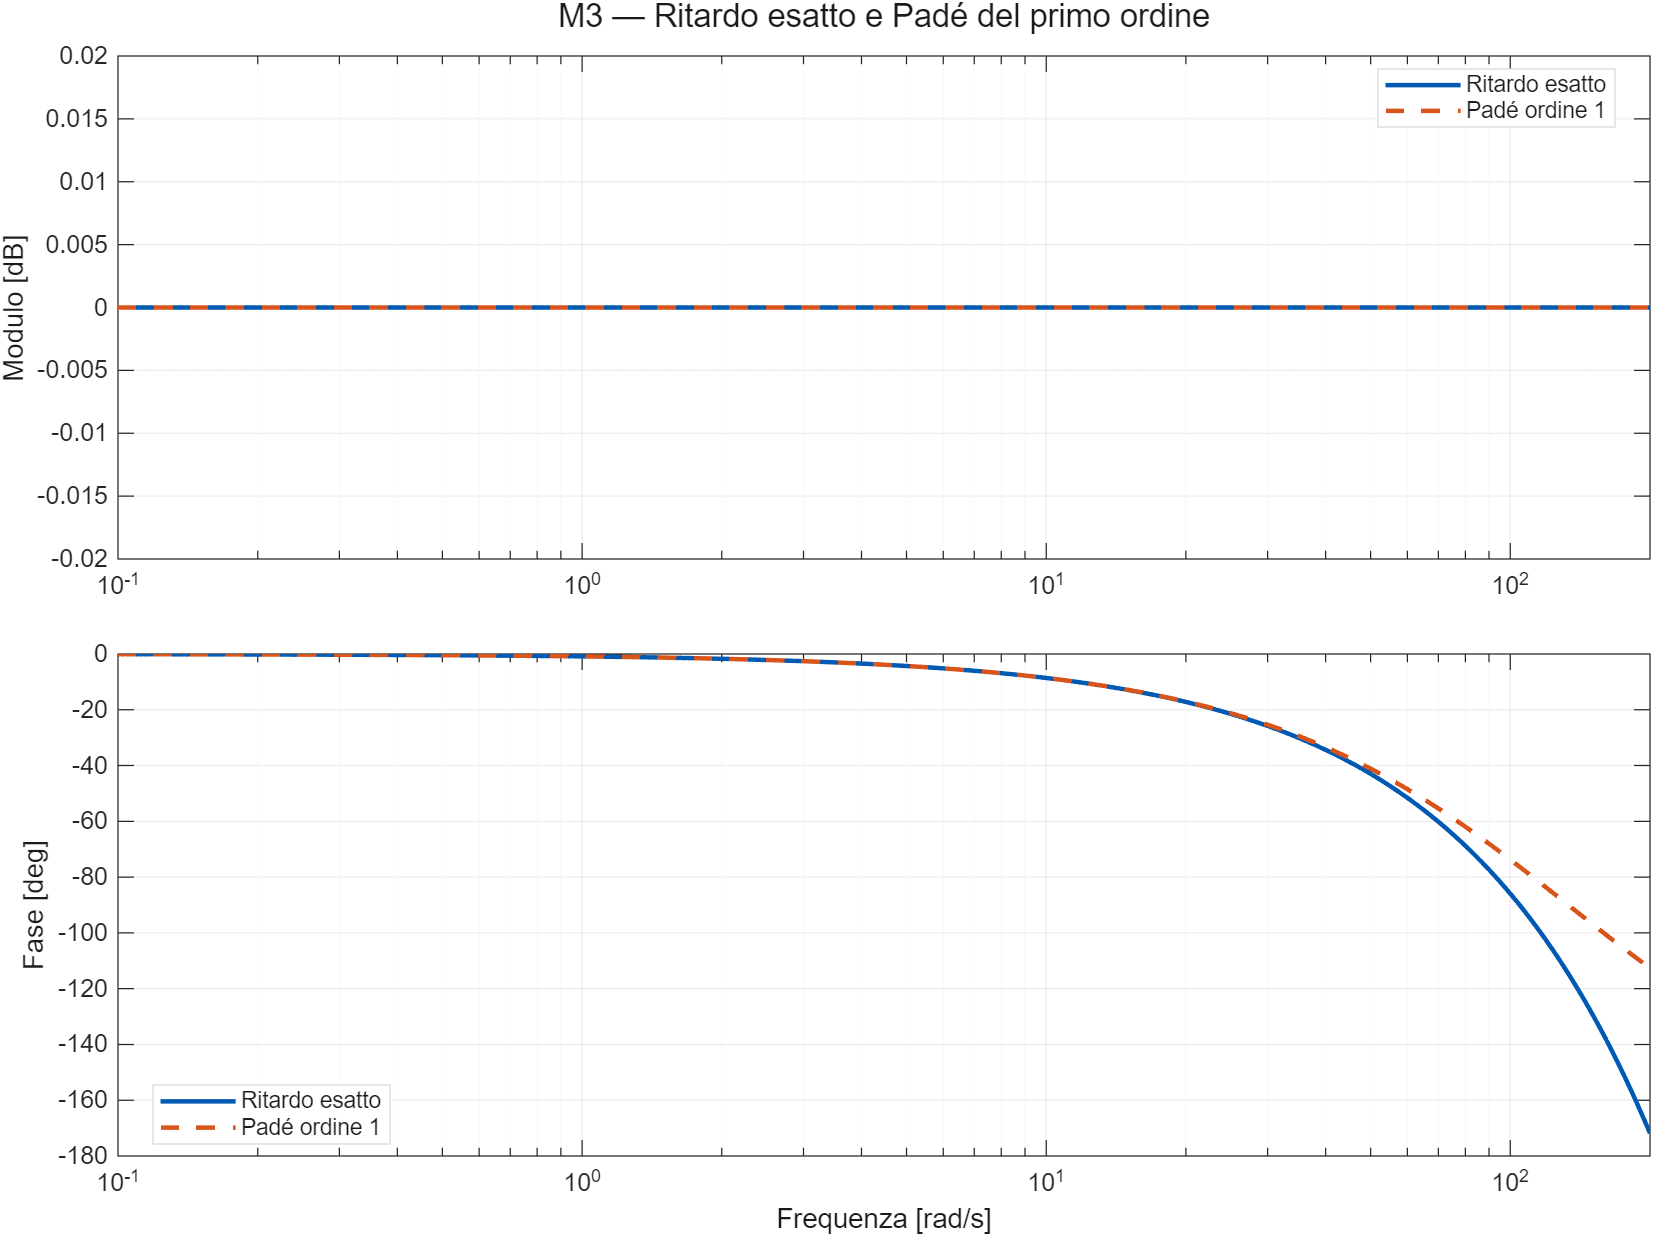
\includegraphics[width=0.76\textwidth]{figures/m3_delay_pade_comparison.png}
\caption{Confronto fra ritardo esatto e Padé del primo ordine (M3).}\label{fig:m3-pade}
\end{figure}

\section{Interconnessione con la meccanica}
Ogni attuatore razionale ha ordine tre; due copie diagonali aggiungono sei stati agli otto stati meccanici. La pianta nominale completa ha quindi ordine \FullPlantOrder. Indicando con $(A_a,B_a,C_a,D_a)$ la realizzazione dei due attuatori e con $(A_m,B_m,C_m,D_m)$ la meccanica, la cascata è costruita esplicitamente per preservare l'ordine degli stati:
\[
A_{full}=\begin{bmatrix}A_m&B_mC_a\\0&A_a\end{bmatrix},\qquad
B_{full}=\begin{bmatrix}B_mD_a\\B_a\end{bmatrix}.
\]
Il comando $u$ attraversa la dinamica attuativa e produce la coppia motore $\tau$. Le coppie di disturbo fisiche introdotte in seguito agiscono invece direttamente sul lato link, evitando di confondere un carico esterno con un errore del comando. La costruzione è stata confrontata in frequenza con una cascata indipendente e coincide entro la precisione numerica.

La pianta completa conserva i due poli meccanici instabili e aggiunge soltanto poli attuativi stabili. Dopo un opportuno scaling temporale, i test SVD e PBH confermano controllabilità e osservabilità dei 14 stati. L'ordine completo viene mantenuto nelle sintesi: non sono effettuate cancellazioni dei modi elastici o dello zero Padé.

\chapter{Modello delle incertezze}
\section{Obiettivo e principio di modellazione}
Il modello incerto deve mantenere i fenomeni fisici rilevanti senza rendere opaca la struttura $\Delta$. Definiamo quindi un solo insieme di progetto. Non esistono scenari gerarchici: ogni percentuale è un'ipotesi ingegneristica, non una tolleranza misurata o un intervallo di confidenza.

\section{Parametri reali \texttt{ureal}}
Le due rigidezze SEA sono incluse perché modificano direttamente coppia elastica e modi flessibili; $J_{m1}$ rappresenta l'incertezza sull'inerzia riflessa del primo azionamento. Tutti e tre i parametri usano la variazione semplice $\pm10\%$:
\begin{verbatim}
k1  = ureal('k1',  p.Ks(1,1), 'Percentage', 10);
k2  = ureal('k2',  p.Ks(2,2), 'Percentage', 10);
Jm1 = ureal('Jm1', p.Jm(1,1), 'Percentage', 10);
\end{verbatim}
Ogni oggetto è riutilizzato in tutte le occorrenze delle equazioni e resta un singolo blocco reale scalare. Gli altri parametri sono nominali per mantenere l'ensemble leggibile; ciò non equivale a dichiararli fisicamente certi.

La scelta di $k_1$ e $k_2$ è legata alla natura SEA: una variazione di rigidezza cambia sia la coppia elastica $K_s(\theta-q)$ sia la posizione dei modi flessibili. $J_{m1}$ rappresenta invece una direzione di incertezza inerziale del drive train. Il valore $\pm10\%$ è un inviluppo ingegneristico semplice, adottato in assenza di dati di identificazione; non è ricavato da una distribuzione statistica. Per evitare di moltiplicare blocchi scarsamente giustificati, $m_1,m_2,l_1,l_2,J_{m2},B_{m1},B_{m2}$ e $g$ restano nominali. Le masse e le geometrie definiscono il modello rigido adottato, $J_{m2}$ non duplica la direzione già rappresentata da $J_{m1}$, gli smorzamenti sono termini dissipativi piccoli e $g$ è una costante ambientale. Questa esclusione è una scelta di modello, non una dichiarazione di certezza fisica.

Un parametro \texttt{ureal} conserva una dipendenza reale e ripetuta: se $k_1$ compare in più elementi di $A$, tutte le occorrenze variano in modo coerente attraverso lo stesso scalare normalizzato. È quindi adatto a una dispersione parametrica strutturata. Un blocco \texttt{ultidyn}, usato più avanti per $W_I\Delta$, descrive invece una dinamica stabile non nota entro un limite in norma; non possiede un unico valore fisico come rigidezza, massa o ritardo.


\medskip\noindent\textbf{Derivazione manuale della LFT meccanica.}
Affianchiamo alla costruzione automatica una rappresentazione ottenuta dalle
equazioni SEA, senza cambiarne equilibrio o parametri. Poniamo
$x=[q^\top,\dot q^\top,\theta^\top,\dot\theta^\top]^\top$,
$t=[\tau^\top,d^\top]^\top$, $K_r=0.1K_{s0}$ e
$j_r=0.1J_{m1,0}e_1$. La coppia elastica incerta è
$K_{s0}(\theta-q)+K_r w_k$, con
$w_k=\operatorname{diag}(\delta_{k1},\delta_{k2})(\theta-q)$.
L'equazione motore si scrive esattamente come
\[
 J_{m0}\ddot\theta=\tau-B_m\dot\theta-K_{s0}(\theta-q)
                   -K_r w_k-j_r w_J,\qquad
 w_J=\delta_J\ddot\theta_1.
\]
Questa chiusura conserva l'inverso dell'inerzia: non sostituisce
$1/J_{m1}$ con una linearizzazione. Con $M_\ell$ matrice d'inerzia
link all'equilibrio e $(A_0,B_0,C_0)$ della meccanica nominale,
\[
 B_w=\begin{bmatrix}
 0_{2\times3}\\ M_\ell^{-1}[K_r\ \ 0]\\0_{2\times3}\\
 -J_{m0}^{-1}[K_r\ \ j_r]
 \end{bmatrix},\qquad
 \dot x=A_0x+B_0t+B_ww_\Delta.
\]
Le porte verso l'incertezza sono
$v_\Delta=[(\theta-q)^\top,\ddot\theta_1]^\top$.
Se $e_7$ seleziona la prima accelerazione motore in $\dot x$,
\[
 C_v=\begin{bmatrix}[-I\  0\  I\  0]\\e_7^\top A_0\end{bmatrix},
 \quad D_{vw}=\begin{bmatrix}0_{2\times3}\\e_7^\top B_w\end{bmatrix},
 \quad D_{vt}=\begin{bmatrix}0_{2\times4}\\e_7^\top B_0\end{bmatrix}.
\]
La parte nota $M_m$ ha realizzazione
$(A_0,[B_w\ B_0],[C_v;C_0], [D_{vw}\ D_{vt};0_{2\times7}])$,
cinque uscite $[v_\Delta;q]$ e sette ingressi $[w_\Delta;t]$.
Il blocco $\Delta_m=\operatorname{diag}(\delta_{k1},\delta_{k2},\delta_J)$
è $3\times3$ e ciascuno scalare appartiene a $[-1,1]$.
La chiusura è ben posta perché $1+0.1\delta_J\ge0.9$.
Nel codice \texttt{lft(Delta,M)} richiude queste prime porte; la
costruzione non usa \texttt{lftdata} per ottenere le matrici manuali.
\begin{center}
\begin{tikzpicture}[>=stealth,thick,every node/.style={font=\small},
 b/.style={draw,rounded corners,align=center,minimum width=4cm,minimum height=1cm}]
\node[b] (m) at (0,0) {$M_m$: meccanica nominale\\porte ricavate dalle equazioni SEA};
\node[b] (d) at (0,2.1) {$\Delta_m=\operatorname{diag}(\delta_{k1},\delta_{k2},\delta_J)$};
\draw[->] (m.east) -- (3.8,0) -- (3.8,2.1) -- node[above] {$v_\Delta$} (d.east);
\draw[->] (d.west) -- (-3.8,2.1) -- (-3.8,0) -- node[above] {$w_\Delta$} (m.west);
\draw[->] (-3,-1.3) node[left] {$t=[\tau;d]$} -- (-1,-1.3) -- (m.south -| -1,0);
\draw[->] (m.south -| 1,0) -- (1,-1.3) -- (3,-1.3) node[right] {$q$};
\end{tikzpicture}

\end{center}
Il confronto con la meccanica automatica usa il nominale, tutti gli otto
vertici e 24 punti interni con seed 20261026. Su 1601 frequenze fra
$10^{-4}$ e $10^5$ rad/s lo scarto relativo massimo è
$1.71\cdot10^{-14}$. La derivazione stabilisce l'identità strutturale;
i campioni ne controllano l'implementazione numerica.

\section{Incertezza dinamica degli attuatori}
Per ciascun drive assumiamo $\omega_n$ e $\zeta$ in $\pm10\%$ e il ritardo in $\pm20\%$. Il ritardo ha un intervallo più ampio perché include latenza e jitter. La famiglia di verifica contiene il nominale con ritardo esatto, sei variazioni singole, otto corner e 105 campioni riproducibili.

La convenzione input-moltiplicativa è
\[
G_{a,i}(s)=G_{a,0}(s)[1+W_I(s)\Delta_i(s)],\qquad
\|\Delta_i\|_\infty\le1.
\]
La forma dell'inviluppo presenta una sola transizione principale; viene perciò scelto un peso di ordine uno e \texttt{ucover} ne calcola i coefficienti. Non viene eseguito un ranking di ordini. Il peso finale è stabile e proprio; la copertura è verificata sui campioni e sulle frequenze della griglia, con safety factor 1.08 e rapporto massimo $|E|/|W_I|=0.92593$.

Il range $\pm10\%$ su $\omega_n$ e $\zeta$ rappresenta la variazione moderata della banda e dello smorzamento al mutare di drive e carico. Sul ritardo si usa $\pm20\%$: la latenza nominale di 15 ms può includere non soltanto dispersioni parametriche, ma anche scheduling e jitter, per i quali un inviluppo relativo più ampio è prudente. Questi tre parametri servono a costruire la famiglia di errori; nella pianta incerta finale la famiglia è condensata nel canale dinamico $W_I\Delta$, evitando di trattare un ritardo come un semplice scalare reale.

I due canali usano $\Delta_{act1}$ e $\Delta_{act2}$ indipendenti. Un unico blocco avrebbe imposto una correlazione perfetta non supportata da dati. La struttura finale è:
% Generated by build_m18_report_tables.m. Do not edit.
\begin{table}[H]
\centering
\resizebox{\textwidth}{!}{%
\begin{tabular}{llll}
\toprule
Parametro & Nominale & Range & Rappresentazione \\
\midrule
k2 & 40 & 7\% & parametrica reale \\
k1 & 50 & 7\% & parametrica reale \\
Jm1 & 0.01 & 9\% & parametrica reale \\
wn & 40 & 8\% & famiglia coperta da $W_I\Delta$ \\
zeta & 0.8 & 7.5\% & famiglia coperta da $W_I\Delta$ \\
delay & 0.015 & 20\% & famiglia coperta da $W_I\Delta$ \\
\bottomrule
\end{tabular}
}
\caption{Incertezze ingegneristiche M4; i range non sono distribuzioni probabilistiche identificate.}
\label{tab:uncertainties}
\end{table}


\begin{figure}[H]\centering
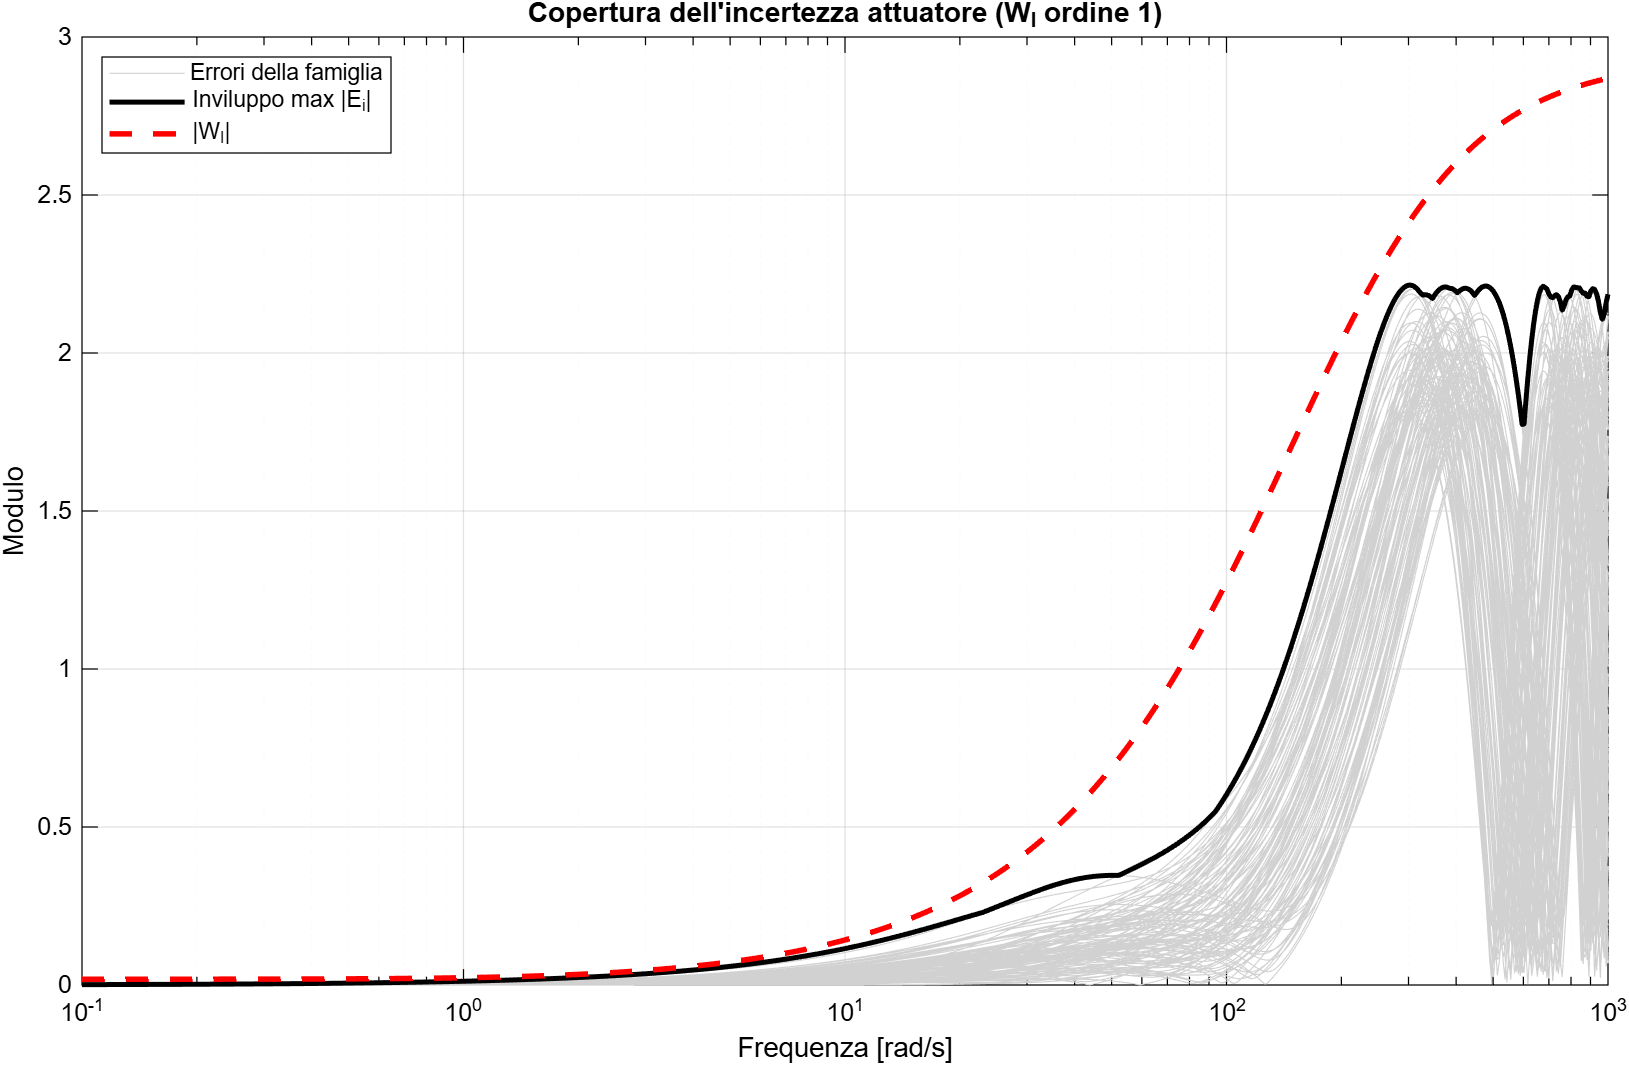
\includegraphics[width=0.78\textwidth]{figures/student_baseline/actuator_uncertainty.png}
\caption{Errore moltiplicativo della famiglia e copertura mediante $W_I$.}\label{fig:m4-wi}
\end{figure}


\medskip\noindent\textbf{Limite della copertura moltiplicativa con Pad\'e.}
La verifica in modulo sulla griglia non dimostra che l'errore normalizzato
sia una dinamica stabile. Con $T_0=0.015$ s, il nominale razionale
$G_{a0}=H_0P_{T_0}$ contiene
\[
 H_{\omega,\zeta}(s)=\frac{\omega^2}{s^2+2\zeta\omega s+\omega^2},
 \qquad P_T(s)=\frac{1-Ts/2}{1+Ts/2}.
\]
$P_{T_0}$ ha uno zero a $s=2/T_0=133.33$ rad/s nel semipiano destro.
Già per il ritardo esatto nominale, $e^{-T_0s}/P_{T_0}(s)-1$
ha un polo in quel punto, con residuo $-4e^{-2}/T_0\ne0$.
Poiché $W_I$ storico non cancella tale polo, la corrispondente
$\Delta$ non appartiene alla classe stabile di \texttt{ultidyn}.
I certificati storici restano validi per il loro modello matematico,
ma la sola copertura frequenziale non li trasferisce all'intera famiglia
con ritardo esatto. Il modello moltiplicativo e i relativi risultati sono
conservati senza ricalcolo o sostituzione degli archivi.

\medskip\noindent\textbf{Due rappresentazioni per lo stesso dominio fisico.}
Il confronto aggiuntivo mantiene $\omega\in[36,44]$ rad/s,
$\zeta\in[0.72,0.88]$ e $T\in[0.012,0.018]$ s, indipendenti per
ciascun attuatore. Sono ritardi costanti incerti; la certificazione non
include jitter arbitrariamente variabile nel tempo. Indichiamo gli estremi
con $\omega_\pm,\zeta_\pm,T_\pm$ e il nominale con il pedice zero.
La rappresentazione parametrica B è
\[
 G_{a,B}=H_{\omega,\zeta}(P_T+W_R\Delta_R),\qquad
 \|\Delta_R\|_\infty\le1,
 \qquad
 W_R=\kappa\left(\frac{T_+s}{1+T_+s}\right)^3,
 \quad \kappa=\frac{(1+24^{2/3})^{3/2}}{12}.
\]
Infatti, per $x=|\Omega T|$,
$|e^{-j\Omega T}-P_T(j\Omega)|\le\min(2,x^3/12)$:
la differenza di fase $x-2\arctan(x/2)$ è al più $x^3/12$.
Il massimo del rapporto tra questa maggiorazione e
$(x/\sqrt{1+x^2})^3$ è $\kappa$.
Il residuo normalizzato ha una singolarità rimovibile all'origine,
è stabile e limitato anche ad alta frequenza. Il residuo fisico dipende
da $T$; renderlo indipendente in B allarga l'insieme e introduce
conservatività dichiarata. Il nominale di B resta $H_0P_{T_0}$:
il ritardo esatto nominale è un altro membro della famiglia, con
$\Delta_R\ne0$.

La LFT manuale usa $x_a, v_a=\dot x_a$ per il secondo ordine e $h$ per
Pad\'e. Con $\omega=\omega_0(1+0.1\delta_\omega)$,
$\zeta=\zeta_0(1+0.1\delta_\zeta)$ e
$T=T_0(1+0.2\delta_T)$, apriamo le porte
\[
 \begin{aligned}
 a&=\omega_0(u-x_a+0.1w_{\omega1}),&
 b&=a-2\zeta_0(v_a+0.1w_\zeta),\\
 \dot v_a&=\omega_0(b+0.1w_{\omega2}),&
 \dot h&=2(x_a-h)/T_0-0.2w_T,\\
 y_P&=2h-x_a,& y_a&=y_P+W_Rw_R,
 \end{aligned}
\]
con $v_\Delta=[u-x_a,b,v_a,\dot h,x_a]^\top$ e
\[
 w_\Delta=\Delta_a v_\Delta,\qquad
 \Delta_a=\operatorname{diag}
 (\delta_\omega I_2,\delta_\zeta,\delta_T,\Delta_R).
\]
Le due occorrenze di $\delta_\omega$ sono lo stesso scalare, non due
incertezze indipendenti: richiudendole si ricostruiscono sia
$\omega^2$ sia $2\zeta\omega$. Il loop di $\delta_T$ produce
$1/T$ esattamente ed è ben posto, poiché $1+0.2\delta_T\ge0.8$.
La matrice nota attuativa è $6\times6$ e $\Delta_a$ è $5\times5$.
Con due attuatori e la meccanica, B ha nove scalari reali distinti e due
blocchi dinamici, con dimensione totale di $\Delta$ pari a 13.
\begin{center}
\begin{tikzpicture}[>=stealth,thick,every node/.style={font=\small},
 b/.style={draw,align=center,minimum width=2cm,minimum height=.8cm}]
\node at (-5.4,1.3) {B};
\node[b] (h) at (-3,0) {$H_{\omega,\zeta}$};
\node[b] (p) at (.6,.8) {$P_T$};
\node[b] (r) at (.6,-.8) {$W_R\Delta_R$};
\node[draw,circle,inner sep=2pt] (s) at (3.3,0) {$+$};
\draw[->] (-5.2,0) node[left] {$u$} -- (h);
\draw[->] (h.east) -- (-1.4,0) |- (p.west);
\draw[->] (-1.4,0) |- (r.west);
\draw[->] (p.east) -| (s.north);
\draw[->] (r.east) -| (s.south);
\draw[->] (s.east) -- (4.7,0) node[right] {$y_a$};
\node at (-5.4,-2.4) {A};
\node[b] (n) at (-.2,-2) {$H_0P_{T_0}$};
\node[b] (a) at (-.2,-3.4) {$W_A\Delta_A$};
\node[draw,circle,inner sep=2pt] (sa) at (3.3,-2.7) {$+$};
\draw[->] (-5.2,-2.7) node[left] {$u$} -- (-3.5,-2.7) |- (n.west);
\draw[->] (-3.5,-2.7) |- (a.west);
\draw[->] (n.east) -| (sa.north);
\draw[->] (a.east) -| (sa.south);
\draw[->] (sa.east) -- (4.7,-2.7) node[right] {$y_a$};
\end{tikzpicture}

\end{center}

La rappresentazione concentrata A raccoglie invece lo scarto additivo
rispetto allo stesso nominale:
\[
 G_{a,A}=H_0P_{T_0}+W_A\Delta_A,\qquad \|\Delta_A\|_\infty\le1.
\]
Per costruire il peso senza il polo spurio dell'inversione di Pad\'e,
definiamo $a=\max_{\omega\in[\omega_-,\omega_+]}|\omega^2-\omega_0^2|$
e $b=\max_{\omega,\zeta}|2\zeta_0\omega_0\omega^2-2\omega_0^2\zeta\omega|$.
Il codice valuta anche gli eventuali punti stazionari interni per $b$.
Usiamo le maggiorazioni stabili
\[
 \begin{aligned}
 W_H(s)&=\frac{\sqrt2\,s(as+b)}
 {\zeta_-(s+\omega_-)^2(s^2+2\zeta_0\omega_0s+\omega_0^2)},\\
 W_T(s)&=\frac{\max(T_+-T_0,T_0-T_-)s}
 {(1+T_-s/2)(1+T_0s/2)},\qquad
 \overline H(s)=\frac{\omega_+^2}{\zeta_-(s+\omega_-)^2}.
 \end{aligned}
\]
Per $0<\zeta_-\le1$ vale
$|(j\Omega)^2+2\zeta\omega j\Omega+\omega^2|
\ge\zeta_-(\omega^2+\Omega^2)$.
La differenza dei due secondi ordini dà quindi
$|H_{\omega,\zeta}-H_0|\le|W_H|$;
inoltre $|P_T-P_{T_0}|\le|W_T|$ e $|H_{\omega,\zeta}|\le|\overline H|$.
Il peso $W_A$ è il fattore spettrale stabile, con zeri nel semipiano
sinistro salvo quello all'origine, definito da
\[
 |W_A|^2=3\bigl(|W_H|^2+|H_0W_T|^2+|\overline H W_R|^2\bigr).
\]
La disuguaglianza $(a_1+a_2+a_3)^2\le3\sum a_i^2$ applicata a
$(H-H_0)P_T+H_0(P_T-P_{T_0})+HW_R\Delta_R$ dimostra
$|G_{a,B}-G_{a0}|\le|W_A|$. La normalizzazione additiva è stabile:
lo zero all'origine è rimovibile e il grado relativo due del peso
è compatibile con gli scarti attuativi. Ne segue
$\mathcal G_{\rm fisica}\subseteq\mathcal G_B\subseteq\mathcal G_A$
per il dominio unitario, senza postulare la stessa inclusione per ogni
scala dei margini robusti. A ha cinque blocchi totali, come numero ma
non come significato uguali al modello storico. Non costituisce una
nuova sintesi o un terzo progetto: serve a misurare la conservatività
della concentrazione rispetto alla rappresentazione parametrica.

\section{Verifica e limiti}
La struttura contiene \MFourBlockCount\ blocchi: tre \texttt{ureal} e due \texttt{ultidyn}. Il valore nominale delle viste verso $[q;\theta]$ e verso $q$ coincide con il modello completo entro $10^{-8}$. Quaranta campioni \texttt{usample} rispettano i range e producono sistemi finiti delle dimensioni attese.

Questa verifica riguarda la costruzione dell'ensemble, non la robustezza in anello chiuso. I range sono intervalli ammissibili, non densità di probabilità: per questo un campionamento uniforme usato nelle prove pratiche non autorizza un'interpretazione probabilistica dei conteggi. Le conclusioni RS/RP appartengono alla $\mu$-analysis. Anche il campionamento successivo resta evidenza empirica e non sostituisce la certificazione strutturata.

Le verifiche aggiuntive, separate dalla campagna storica, confrontano le due
LFT attuative con una realizzazione automatica indipendente su otto vertici
e 24 punti interni per canale, includendo un residuo dinamico stabile non
nullo. Lo scarto massimo è $1.45\cdot10^{-15}$; il fattore spettrale
soddisfa l'identità con errore relativo $1.05\cdot10^{-14}$ su 2401
frequenze. Nei campioni fisici i massimi rapporti residuo/$W_R$ e scarto/$W_A$
sono 0.885 e 0.339. Questi ultimi sono controlli numerici, mentre la
copertura continua discende dalle disuguaglianze precedenti. Il confronto
a controllore fissato è discusso nel Capitolo 9; non modifica $W_e,W_u,M_o$.

\chapter{Specifiche e pesi di prestazione}
\section{Obiettivo e scenari}
Le specifiche traducono il problema fisico in obiettivi comuni alle sintesi. Il riferimento nominale è un gradino articolare di $5^\circ$ attorno all'equilibrio; le ampiezze 2, 5 e $8^\circ$ servono soltanto a verificare la località del modello. Il disturbo nominale è una coppia di 0.5 N m applicata direttamente ai link. I target principali sono
\[
T_s\le\SettlingTarget\ \mathrm{s},\quad M_p\le\OvershootTarget\%,
\quad e_{ss}\le\ErrorTargetPct\%,\quad c_{cross}\le\CrossTargetPct\%.
\]
% Generated by build_m18_report_tables.m. Do not edit.
\begin{table}[H]
\centering
\begin{tabular}{lll}
\toprule
Quantita & Target & Unita/nota \\
\midrule
Settling time & $T_s \leq$ 0.8 & s \\
Overshoot & $M_p \leq$ 10 & \% \\
Errore a regime & $e_{ss} \leq$ 5 & \% \\
Cross-coupling & picco $\leq$ 25 & \% \\
Banda di progetto & 12 & rad/s \\
Scala del comando & 12 & N m (normalizzazione) \\
\bottomrule
\end{tabular}
\caption{Specifiche e normalizzazioni congelate M5.}
\label{tab:specifications}
\end{table}


\section{Scelta della banda}
Il polo instabile dominante è $7.209$ rad/s, la banda attuatore $34.78$ rad/s e il primo modo elastico $69.95$ rad/s. Il valore scelto
\[
\omega_B=12\ \mathrm{rad/s}
\]
cade nella finestra 10.81--13.91 rad/s: è sopra la dinamica instabile e sotto i limiti attuativi ed elastici. La scelta è dichiarata e poi verificata; non viene ricavata da una classifica di candidati.

Questa posizione della banda esprime un compromesso preciso. Scendere verso il polo instabile renderebbe il recupero dell'equilibrio lento e fragile; salire verso la banda dell'attuatore o il primo modo elastico richiederebbe più comando proprio dove ritardo, flessibilità e incertezza dinamica diventano più rilevanti. Il valore non pretende di essere l'unico possibile: è la specifica congelata rispetto alla quale tutti i controllori vengono confrontati.

\section{Peso sulla sensibilità}
Con $S=(I+GK)^{-1}$ adottiamo
\[
W_1(s)=\frac{s/M_s+\omega_B}{s+\omega_BA_s},qquad
A_s=0.05,\quad M_s=2.
\]
Ponendo $s=0$ si ottiene
\[
W_1(0)=\frac{1}{A_s}=20.
\]
Pertanto $\|W_1S\|_\infty<1$ richiede una sensitivity dell'ordine del 5\% alle basse frequenze. Dividendo numeratore e denominatore per $s$ e passando al limite,
\[
W_1(\infty)=\frac{1}{M_s}=0.5.
\]
Il vincolo lascia quindi un picco di sensitivity dell'ordine di $M_s=2$; $\omega_B$ colloca la transizione tra accuratezza statica e roll-off.

La lettura del peso deve essere fatta attraverso il suo inverso. Se $\|W_1S\|_\infty<1$, allora $\bar\sigma(S)<1/|W_1|$: a bassa frequenza l'errore deve essere piccolo, nella zona di transizione si fissa la rapidità desiderata e ad alta frequenza il vincolo si rilassa. Non si tenta quindi di rendere $S$ piccolo a tutte le frequenze, cosa incompatibile con il roll-off e con i limiti di robustezza.

\section{Peso sul comando}
La scala $u_{scale}=12$ N m è una normalizzazione prestazionale, non una saturazione hardware. Usiamo
\[
W_2(s)=\frac{1}{u_{scale}}
\frac{s/\omega_U+1}{s/(\alpha\omega_U)+1},qquad
\omega_U=30\ \mathrm{rad/s},\quad\alpha=6.
\]
A bassa frequenza $W_2(0)=1/12$; ad alta frequenza tende a $\alpha/12=0.5$. La penalizzazione del comando cresce quindi di un fattore sei prima dei modi elastici, scoraggiando azioni rapide nella regione in cui ritardo e flessibilità rendono il modello meno affidabile.

Anche qui il limite è $1/|W_2|$. Alle basse frequenze il comando può sfruttare la scala di 12 N m; oltre $\omega_U$ il bound si riduce fino a circa 2 N m. Questa forma non simula un saturatore e non prova la compatibilità con una curva coppia--velocità reale: introduce soltanto una misura normalizzata dello sforzo di controllo nel problema $H_\infty$.

\section{Implementazione e interpretazione}
I pesi MIMO sono due copie diagonali dei pesi SISO e non viene usato $W_3$. La mixed sensitivity è
\[
\left\|\begin{bmatrix}W_1S\\W_2KS\end{bmatrix}\right\|_\infty.
\]
I test verificano stabilità, properness, dimensioni e asintoti. Il valore uno separa soddisfacimento e violazione del profilo pesato. Le specifiche restano congelate anche quando una sintesi produce $\gamma>1$: il risultato negativo documenta la difficoltà del problema e non giustifica un retuning retroattivo.

La stessa M5 alimenta anche la sintesi LQR: ampiezza del riferimento, banda, coppia di disturbo e scala del comando costruiscono normalizzazioni fisiche comuni. Questo non rende equivalenti LQR e mixed sensitivity; garantisce però che il confronto successivo non usi unità o obiettivi ricavati a posteriori per favorire un controllore.

\begin{figure}[H]\centering
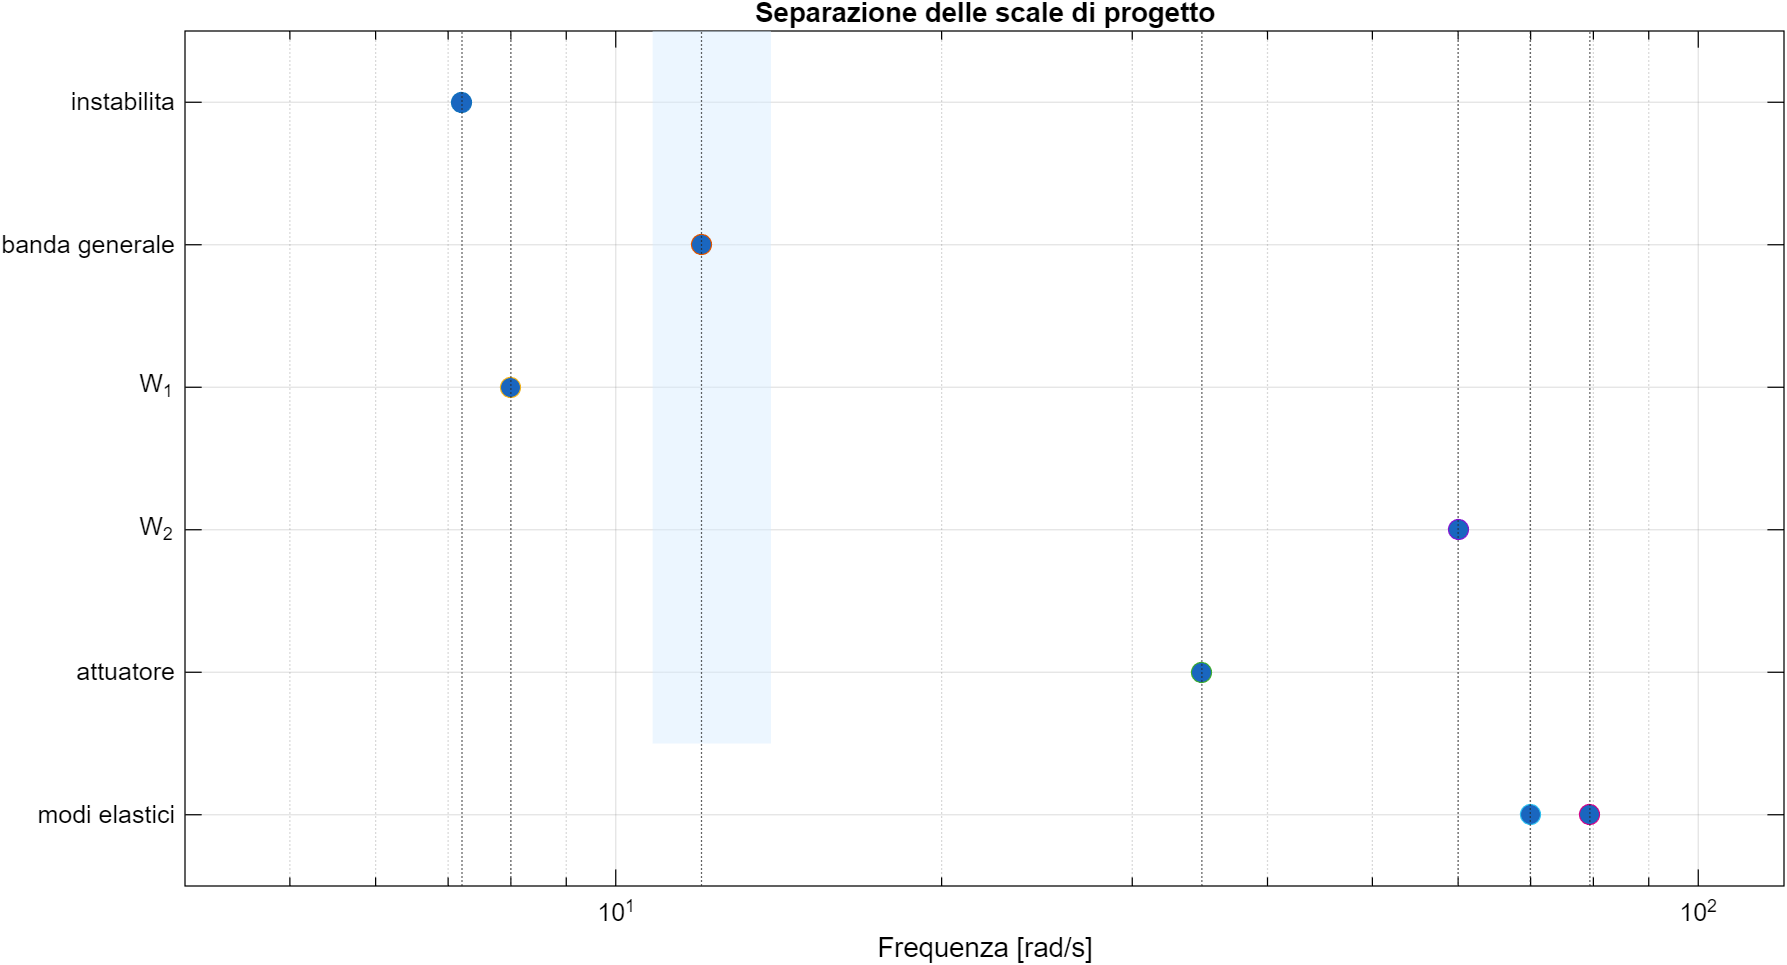
\includegraphics[width=0.79\textwidth]{figures/m5_spec_frequency_map.png}
\caption{Scale dinamiche utilizzate per motivare $\omega_B$ e $\omega_U$.}\label{fig:m5-map}
\end{figure}

\chapter{Controllo LQG}
\section{Obiettivo e architettura}
Il regolatore usa il modello nominale M3 a 14 stati e le quattro misure encoder
$y=[\Delta q^T,\Delta\theta^T]^T$. Le velocità e gli stati interni degli attuatori
non sono misurati. LQR progetta il feedback supponendo lo stato disponibile;
Kalman lo ricostruisce da modello, ingressi e misure. La legge effettivamente
implementata è $u=-K\hat x+N_rr$, nelle coordinate incrementali M2.
Il prefiltro rende unitario il guadagno statico nominale riferimento--posizione,
ma non contiene un modello interno dei disturbi costanti.

\section{Scelta e normalizzazione di Q e R}
\subsection{Il problema LQR e le unità fisiche}
Il costo è
\[
J=\int_0^\infty \left(x^TQx+u^TRu\right)\,dt .
\]
Il primo termine penalizza gli scostamenti delle coordinate fisiche di interesse;
il secondo penalizza le coppie di comando. Il compromesso fra transitorio e
sforzo dipende da entrambi. Usare una matrice identità senza spiegazione
assegnerebbe lo stesso coefficiente numerico a radianti, radianti al secondo e
coordinate arbitrarie di realizzazione, senza renderne comparabili gli effetti.

Lo stato completo, in deviazione dall'equilibrio, è
\[
x=[\Delta q_1,\Delta q_2,\Delta\dot q_1,\Delta\dot q_2,
\Delta\theta_1,\Delta\theta_2,\Delta\dot\theta_1,\Delta\dot\theta_2,x_a^T]^T.
\]
I sei elementi di $x_a$ appartengono alla realizzazione \texttt{ss} dei due
attuatori secondo ordine--Padé; le loro unità dipendono dalla realizzazione,
non sono ulteriori posizioni fisiche. Non viene attribuita loro una scala
meccanica inventata e non ricevono una penalizzazione diretta. Restano comunque
nel modello, nel feedback e nella verifica di stabilità.

\subsection{Scale e provenienza: il significato esatto di qs}
Distinguiamo parametri imposti dalla traccia (A), derivati matematicamente (B),
ricavati da grandezze fisiche (C), scelti nel progetto (D) e selezionati dalla
ricerca (E). Questa distinzione evita di attribuire al docente scelte nostre.

\begin{table}[H]\centering\small
\begin{tabular}{p{3.4cm}p{3.5cm}p{6.6cm}}\toprule
Grandezza del costo & Scala & Origine e significato\\\midrule
$\Delta q_i$ [rad] & $q_s=5\pi/180$ & C da M5-D: ampiezza del riferimento nominale.\\
$\Delta\dot q_i$ [rad/s] & $\dot q_s=12q_s$ & C: velocità caratteristica banda per ampiezza; non velocità massima.\\
$\Delta\theta_i-\Delta q_i$ [rad] & $\delta_s=0.5/40=0.0125$ & C da coppia di disturbo M5-D e rigidezza minima della traccia-A. Scala comune della molla più cedevole.\\
$\Delta\dot\theta_i$ [rad/s] & $\dot\theta_s=\dot q_s$ & D/C: stessa scala cinematica scelta per i motori; non un vincolo.\\
$x_a$ (6 coordinate) & nessuna scala diretta & Nessuna penalizzazione diretta di coordinate dipendenti dalla realizzazione.\\
\bottomrule\end{tabular}
\caption{Scale del costo M6: derivazioni fisiche basate su scelte M5, non nuovi limiti hardware.}
\end{table}

Nel codice di produzione \path{build_lqr_state_cost.m} l'assegnazione è:
\begin{verbatim}
scales.q = m5Spec.referenceAmplitude;
\end{verbatim}
Nel file didattico la medesima
grandezza è chiamata \texttt{qs} e definita nella sezione 5.
Quindi $q_s=\RevQs$ rad è una \emph{scala dimensionale}, non un peso relativo,
non un candidato di tuning e non un risultato della ricerca.
Il peso adimensionale sulla posizione si chiama invece $w_q$.
La scala di velocità effettiva è \RevQds\ rad/s; quella di deformazione
è \RevDeltaScale\ rad. $\Delta\theta$ non viene pesata isolatamente:
entra attraverso la deformazione $\Delta\theta-\Delta q$.

\subsection{Trasformazione esplicita e matrice Q non diagonale}
Introduciamo le otto uscite fisiche del costo:
\[
v=Fx=\begin{bmatrix}\Delta q\\\Delta\dot q\\
\Delta\theta-\Delta q\\\Delta\dot\theta\end{bmatrix},\qquad
F=\begin{bmatrix}
I_2&0&0&0&0\\0&I_2&0&0&0\\-I_2&0&I_2&0&0\\0&0&0&I_2&0
\end{bmatrix}.
\]
L'ultima colonna a blocchi ha sei colonne scalari. Le posizioni sono quindi
penalizzate sia come errore articolare sia come parte della deformazione.
Definiamo
\[
S_x=\operatorname{diag}(q_sI_2,\dot q_sI_2,\delta_sI_2,\dot\theta_sI_2),
\quad \tilde v=S_x^{-1}Fx,\quad
W_q=\operatorname{diag}(w_qI_2,w_vI_2,w_\delta I_2,w_vI_2).
\]
Qui $S_x$ è $8\times8$ perché normalizza le uscite del costo, non uno stato
trasformato invertibile di dimensione 14. Ne segue esattamente
\[
x^TQx=\tilde v^TW_q\tilde v,\qquad
Q=F^TS_x^{-T}W_qS_x^{-1}F=C_{cost}^TC_{cost},\quad
C_{cost}=W_q^{1/2}S_x^{-1}F.
\]
Per ogni uscita normalizzata il coefficiente è $w_i/s_i^2$.
Espandendo il termine elastico compaiono coefficienti incrociati negativi fra
$q_i$ e $\theta_i$. Pertanto scrivere semplicemente $Q=\operatorname{diag}(q_i)$
sarebbe errato per questo progetto. $Q$ è semidefinita positiva: il blocco
attuativo nullo non implica assenza degli attuatori dalla dinamica ottimizzata.

\subsection{R: scala di comando e peso di progetto}
Le due componenti di $u$ sono coppie di comando in N m. Si pone
\[
S_u=\operatorname{diag}(12,12)\ \mathrm{N\,m},\quad
\tilde u=S_u^{-1}u,\quad W_u=\rho_U I_2,\quad
R=S_u^{-T}W_uS_u^{-1}.
\]
La scala 12 N m proviene da M5: è una scelta prestazionale D per normalizzare
il comando, non una coppia massima nominale del motore né un dato sperimentale.
Il coefficiente $\rho_U$ è invece un peso adimensionale di tuning.
Il termine $u^TRu$ equivale quindi a $\rho_U\|\tilde u\|^2$.
La scelta finale $\rho_U=16$ produce $R=(16/144)I_2=(1/9)I_2$.

\subsection{Ricerca semplice: ammissibilità prima del compromesso}
Si conserva la ricerca già approvata, senza nuovi candidati:
\[
w_q\in\{0.5,1,2\},\quad w_v\in\{0.5,1\},\quad
w_\delta\in\{0.1,0.5\},\quad \rho_U\in\{4,8,16\}.
\]
Le scale rimangono costanti. Questi intervalli esplorano variazioni moderate di
priorità di posizione, smorzamento, deformazione e comando; sono scelte D,
non conseguenze univoche delle equazioni fisiche. Per ciascuno dei 36 candidati
si calcolano $Q,R,K,N_r$, si verifica $A-BK$ e si simulano separatamente i due
gradini di 5 gradi, da stato nullo e senza disturbi, su $0:0.002:3$ s.
Si prendono le metriche peggiori dei due giunti.

Sono ammissibili solo i candidati con poli a parte reale $<-10^{-8}$,
$T_s\le0.8$ s, overshoot $\le10\%$, errore statico relativo $\le0.05$ e
residuo del prefiltro finito. $T_s$ usa la banda del 2\% del riferimento
attorno al valore finale nominale. Cross-coupling e comando non vengono
trasformati in nuovi vincoli obbligatori. Fra i candidati ammissibili si minimizza
\[
J_N=0.30\frac{T_s}{0.8}+0.20\frac{M_p}{10}
+0.10\frac{e_{ss}}{0.05}+0.10\frac{c}{0.25}
+0.15\frac{u_{pk}}{12}+0.15\frac{u_{rms}}{12}.
\]
I coefficienti dello score sono priorità progettuali D e sommano a uno.
Il cross-coupling è il rapporto fra picco del giunto non comandato e picco
del giunto comandato; $u_{pk}$ è il massimo assoluto delle coppie e
$u_{rms}$ la radice della media dei quadrati su tempi e canali.
Restano \MLqrAdmissibleCount/\MLqrCandidateCount\ candidati.
Il minimo seleziona \MLqrSelectedCandidate\ (E):
$w_q=2$, $w_v=1$, $w_\delta=0.1$, $\rho_U=16$ e
$J_N=\MLqrSelectedScore$. Non si è eseguito un nuovo retuning.

\begin{figure}[H]\centering
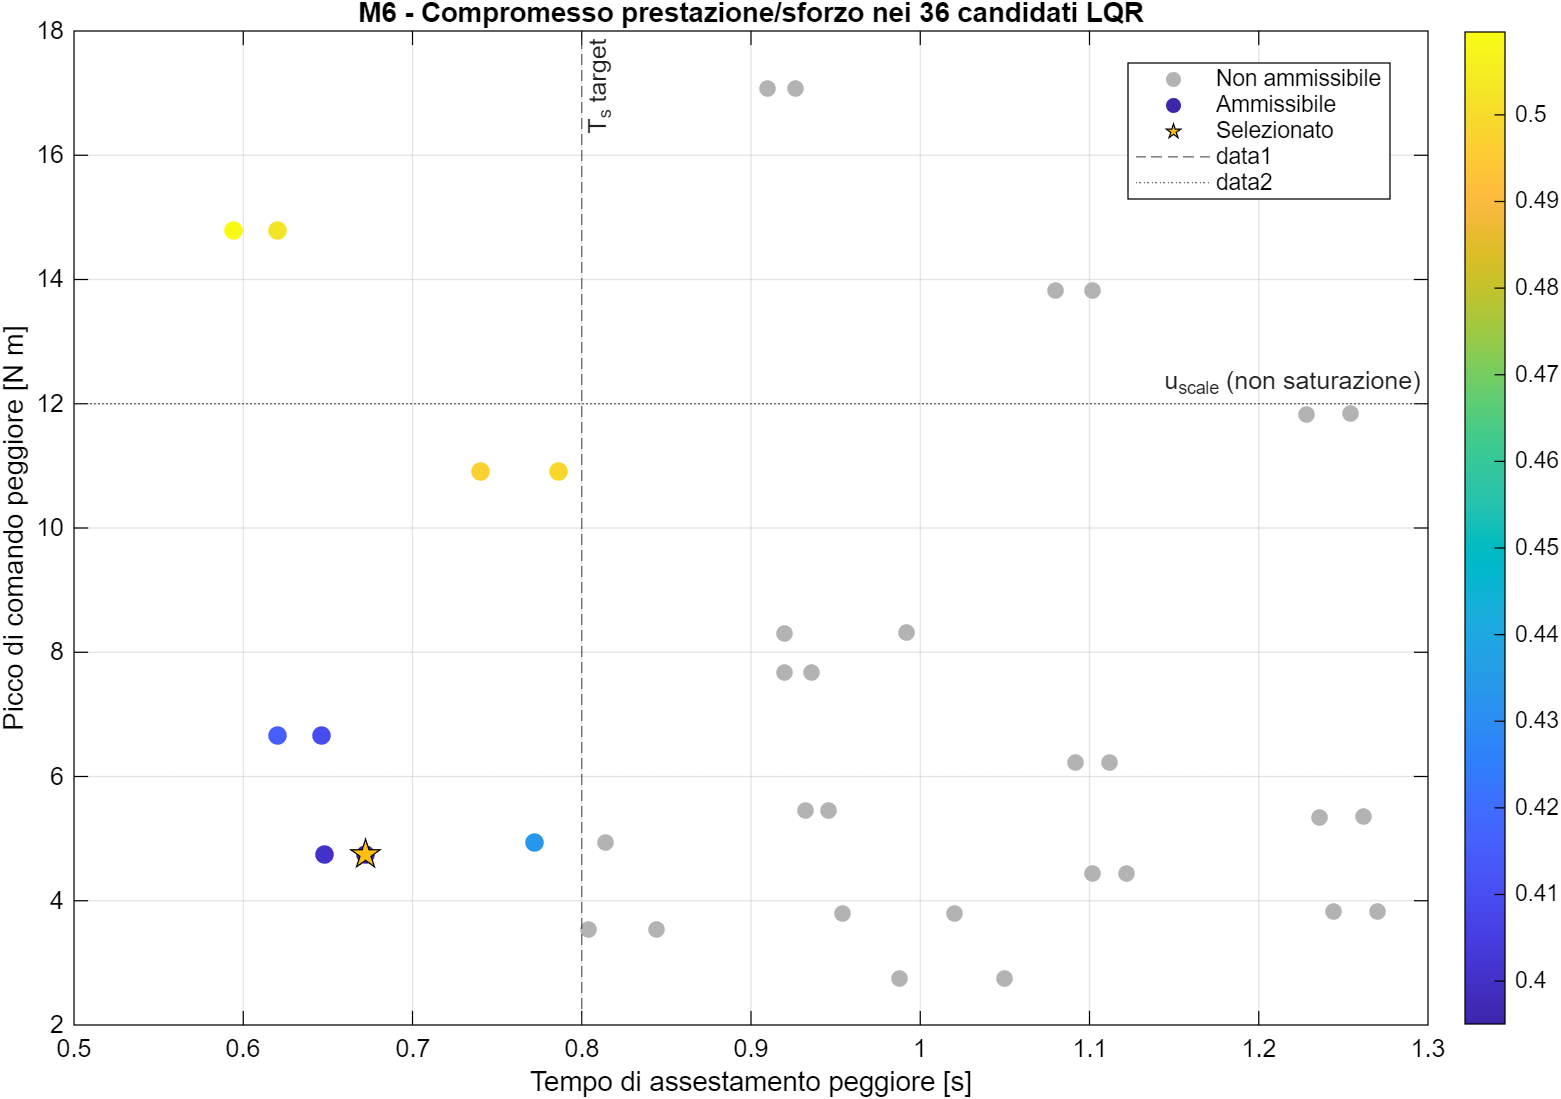
\includegraphics[width=0.78\textwidth]{figures/m6_lqr_candidate_tradeoff.png}
\caption{Ogni punto deriva dai due gradini nominali di un candidato LQR:
ascissa $T_s$ peggiore, ordinata picco di coppia; il colore indica lo score dei
candidati ammissibili e il simbolo evidenzia quello selezionato.
La linea a 12 N m è una scala, non una saturazione.}
\label{fig:m6-lqr-search}
\end{figure}
\begin{figure}[H]\centering
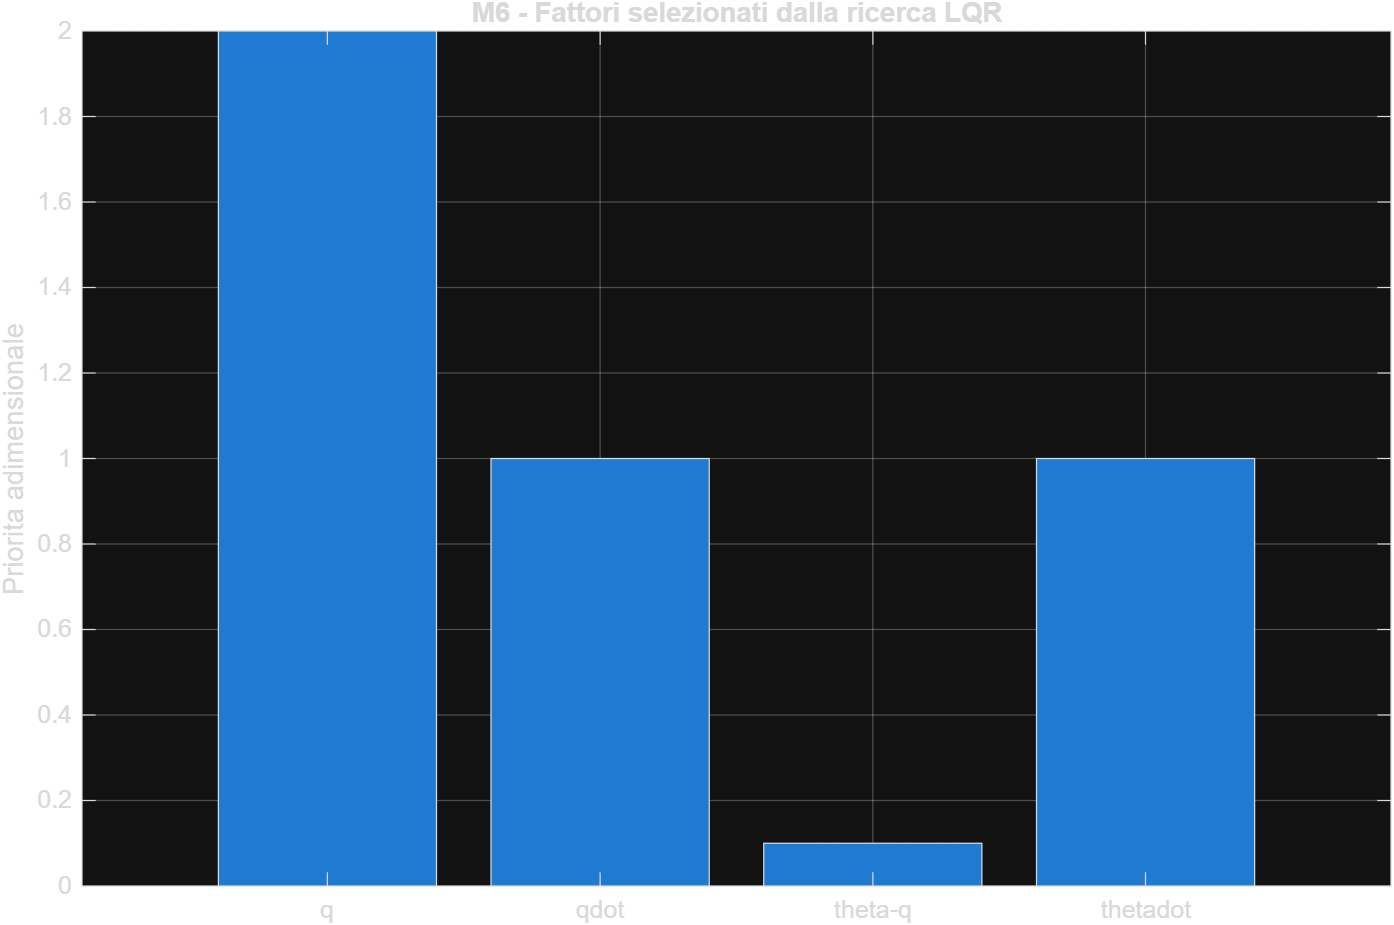
\includegraphics[width=0.70\textwidth]{figures/m6_lqr_selected_weights.png}
\caption{Priorità adimensionali selezionate, da non confondere con le scale fisiche
né con i singoli elementi della matrice non diagonale $Q$.}\label{fig:m6-lqr-weights}
\end{figure}

\subsection{Q e R finali, Riccati, guadagno e stabilità}
MATLAB risolve l'equazione algebrica di Riccati:
\[
A^TP_{\mathrm{LQR}}+P_{\mathrm{LQR}}A
-P_{\mathrm{LQR}}BR^{-1}B^TP_{\mathrm{LQR}}+Q=0,\qquad
K=R^{-1}B^TP_{\mathrm{LQR}}.
\]
$P_{\mathrm{LQR}}$ non è la matrice di Lyapunov introdotta nel Capitolo 10.
Le matrici seguenti provengono dallo script eseguito, arrotondate a cinque cifre
significative; gli artifact conservano la doppia precisione.
% Generato da build_technical_revision_tables, non modificare.
\[Q=\operatorname{blkdiag}(Q_8,0_{6\times6}),\qquad R=\tfrac{1}{9}I_2.\]
{\small
\[
Q_8=\begin{bmatrix}
902.62 & 0 & 0 & 0 & -640 & 0 & 0 & 0 \\
0 & 902.62 & 0 & 0 & 0 & -640 & 0 & 0 \\
0 & 0 & 0.91189 & 0 & 0 & 0 & 0 & 0 \\
0 & 0 & 0 & 0.91189 & 0 & 0 & 0 & 0 \\
-640 & 0 & 0 & 0 & 640 & 0 & 0 & 0 \\
0 & -640 & 0 & 0 & 0 & 640 & 0 & 0 \\
0 & 0 & 0 & 0 & 0 & 0 & 0.91189 & 0 \\
0 & 0 & 0 & 0 & 0 & 0 & 0 & 0.91189 \\
\end{bmatrix}
\]
\[K=[K_a\ K_b],\quad K_a=K(:,1{:}7),\quad K_b=K(:,8{:}14).\]
\[
K_a=\begin{bmatrix}
238.32 & 15.153 & 18.091 & 3.653 & -154.27 & -12.282 & -1.2845 \\
14.6 & 200.59 & 4.4912 & 7.0445 & -5.6235 & -133.66 & -0.61277 \\
\end{bmatrix}
\]
\[
K_b=\begin{bmatrix}
-0.87229 & 11.16 & 21.126 & 39.687 & -0.96424 & -2.3084 & -12.957 \\
1.2023 & -0.96424 & -2.1764 & -10.461 & 13.925 & 27.556 & 75.884 \\
\end{bmatrix}
\]
\[
N_r=\begin{bmatrix}
51.688 & -1.1626 \\
3.2384 & 49.052 \\
\end{bmatrix}
\]
}

La norma del residuo CARE è \RevCareResidual; il polo dominante del regolatore
ha parte reale $-\RevRegulatorDecay$ s$^{-1}$. Tutti i poli di $A-BK$ sono
strettamente nel semipiano sinistro. Il collegamento verificato è dunque
$Q,R\to P_{\mathrm{LQR}}\to K\to A-BK\to$ risposte temporali.
Il prefiltro è $N_r=[-C_q(A-BK)^{-1}B]^{-1}$: garantisce tracking statico
nominale, non reiezione esatta di disturbi costanti.

\section{Filtro di Kalman: ipotesi, covarianze e verifica}
\subsection{Stima dello stato e innovazione}
LQR richiede $x$, mentre sono disponibili soltanto le quattro posizioni.
Il modello usato per la stima è
\[
\dot x=Ax+Bu+G_ww,\qquad y=Cx+v,\qquad G_w=[B_d\ B].
\]
I primi due canali di $w$ sono coppie equivalenti lato link, i successivi due
coppie equivalenti all'ingresso attuativo. I quattro canali di $v$ rappresentano
gli encoder di $q$ e $\theta$. Sono ipotizzati indipendenti, a media nulla,
senza correlazione processo--misura. Lo stimatore realizza
\[
\dot{\hat x}=A\hat x+Bu+L(y-C\hat x).
\]
L'innovazione $y-C\hat x$ confronta la misura con la previsione del modello:
il guadagno $L$ stabilisce quanto questa differenza corregga ciascuno stato.

\subsection{Origine delle sigma e costruzione non ambigua delle covarianze}
Non sono disponibili dati sperimentali sui sensori o sugli errori di processo.
Le scale
$\sigma_d=0.1$ N m, $\sigma_u=0.1$ N m e $\sigma_y=0.05^\circ$
sono ipotesi progettuali D di questo lavoro, \emph{non dati del docente}.
Il loro scopo è assegnare fiducia relativa al modello e alle misure, non
rappresentare una caratterizzazione dell'hardware.
Per contestualizzarle, 0.1 N m equivale al 20\% del disturbo M5 e allo 0.83\%
della scala di comando; 0.05 gradi equivale all'1\% del riferimento.
Questi rapporti descrivono i valori già scelti: non sono una legge fisica che
li determini univocamente. La sensibilità successiva ne rende verificabili
le conseguenze senza un'ottimizzazione delle covarianze.

La varianza è il quadrato della deviazione standard. La costruzione effettiva è
\[
Q_n=\operatorname{diag}(\sigma_d^2,\sigma_d^2,\sigma_u^2,\sigma_u^2)
=0.01\,I_4,\qquad
R_n=(0.05\pi/180)^2I_4=\RevRn\,I_4.
\]
$Q_n$ agisce sui quattro canali di $w$, non direttamente sui 14 stati;
la covarianza equivalente nello stato è $G_wQ_nG_w^T$.
La notazione $0.01 I_4$ evita ogni ambiguità fra $(0.1)^2$ e $0.12$.

Una precisazione è necessaria per il filtro continuo: il rumore bianco ideale
non ha una deviazione standard istantanea finita. In \texttt{lqe}, $Q_n,R_n$
sono intensità, ossia coefficienti della delta di Dirac nelle correlazioni.
Le sigma sopra sono scale equivalenti riferite alla convenzione temporale di
1 s; restituendo le dimensioni temporali, le intensità hanno unità
$(\mathrm{N\,m})^2\,\mathrm{s}$ e $\mathrm{rad}^2\,\mathrm{s}$.
La successiva simulazione \texttt{randn} usa invece campioni con deviazione
standard finita a passo 2 ms. Non viene affermata l'equivalenza di questo
esperimento con il modello bianco continuo né una calibrazione probabilistica.

\subsection{Guadagno, poli e sensibilità a ingresso identico}
Il calcolo eseguito è
$\texttt{L=lqe(A,Gw,C,Qn,Rn)}$. La matrice seguente segue l'ordine degli stati
M3 per le righe e $[q_1,q_2,\theta_1,\theta_2]$ per le colonne:
{\small
\[
L=\begin{bmatrix}
22.709 & -21.794 & 9.0441 & -5.5227 \\
-21.794 & 85.604 & -6.9226 & 23.471 \\
551.47 & -1274.4 & 233.27 & -349.38 \\
-1278.4 & 4200.9 & -381.6 & 1210.6 \\
9.0441 & -6.9226 & 64.38 & -3.4219 \\
-5.5227 & 23.471 & -3.4219 & 79.196 \\
724.13 & -934.1 & 2143.1 & -313.45 \\
-755.87 & 2801.5 & -390.28 & 3432.6 \\
-0.41526 & -2.2541 & -35.115 & -1.7286 \\
24.32 & 14.409 & -92.137 & -0.28863 \\
-30.066 & -12.673 & 207.83 & 4.7948 \\
-1.9579 & 4.8133 & -1.7025 & -30.032 \\
11.54 & -9.1651 & 1.3605 & -101.99 \\
-9.7589 & -0.59062 & 2.617 & 207.42 \\
\end{bmatrix}
\]
}

I poli di $A-LC$ sono stabili; la velocità asintotica minima vale
$\alpha_e=\RevEstimatorDecay$ s$^{-1}$, contro
$\alpha_c=\RevRegulatorDecay$ s$^{-1}$ del regolatore.
Il rapporto è \MKalmanSpeedRatio, non un requisito imposto dal docente.

Nella nuova verifica si varia soltanto il rumore \emph{assunto} dallo stimatore:
$0.5\sigma_y,\sigma_y,2\sigma_y$, cioè $R_n/4,R_n,4R_n$.
$Q_n$ e LQR restano invariati. Si applica a tutti la stessa sequenza encoder,
con $\sigma_y=0.05^\circ$, seed 20260826, 4 s a passo 2 ms, riferimento
$r_1=5^\circ,r_2=0$, stato iniziale nullo e nessun disturbo di coppia.
\begin{table}[H]\centering\small
\begin{tabular}{rrrrr}\toprule
$\sigma_{y,ass}/\sigma_y$ & $\alpha_e/\alpha_c$ & RMS $e_q$ [rad] & RMS $\Delta u$ [N m] & $\|G_{v\to C_{cost}e}\|_2$ \\
\midrule
0.5 & 2.0962 & 0.00029595 & 0.14991 & 1065.8 \\
1 & 1.4985 & 0.00023377 & 0.08195 & 718.29 \\
2 & 1.1833 & 0.00018109 & 0.042779 & 486.49 \\
\bottomrule\end{tabular}
\caption{Sensibilit\`a a parit\`a di rumore applicato: seed 20260826, $\sigma_y=0.05^\circ$, passo 2 ms, 4 s. Varia solo $R_n$ assunto.}\label{tab:kalman-fixed}
\end{table}

Il filtro che assume misure più affidabili è più rapido, ma nella prova
a rumore identico amplifica maggiormente le fluttuazioni di stima e comando.
Aumentare relativamente $R_n$ tende a filtrare di più; aumentare relativamente
$Q_n$ tende a valorizzare l'innovazione. Questa è una tendenza complessiva:
nel caso MIMO non implica monotonia di ogni polo o elemento di $L$.
La norma $\mathcal H_2$ è quella della mappa
$v\to C_{cost}(x-\hat x)$ a ingresso unitario, non un RMS fisico del sensore.

L'esperimento precedente, conservato nelle colonne storiche dell'artifact,
variava anche l'ampiezza del rumore applicato: confrontava scenari diversi.
Le nuove colonne \texttt{RmsEstimationErrorFixedNoise} e
\texttt{RmsControlFixedNoise} isolano invece l'effetto della sola covarianza assunta.
\begin{figure}[H]\centering
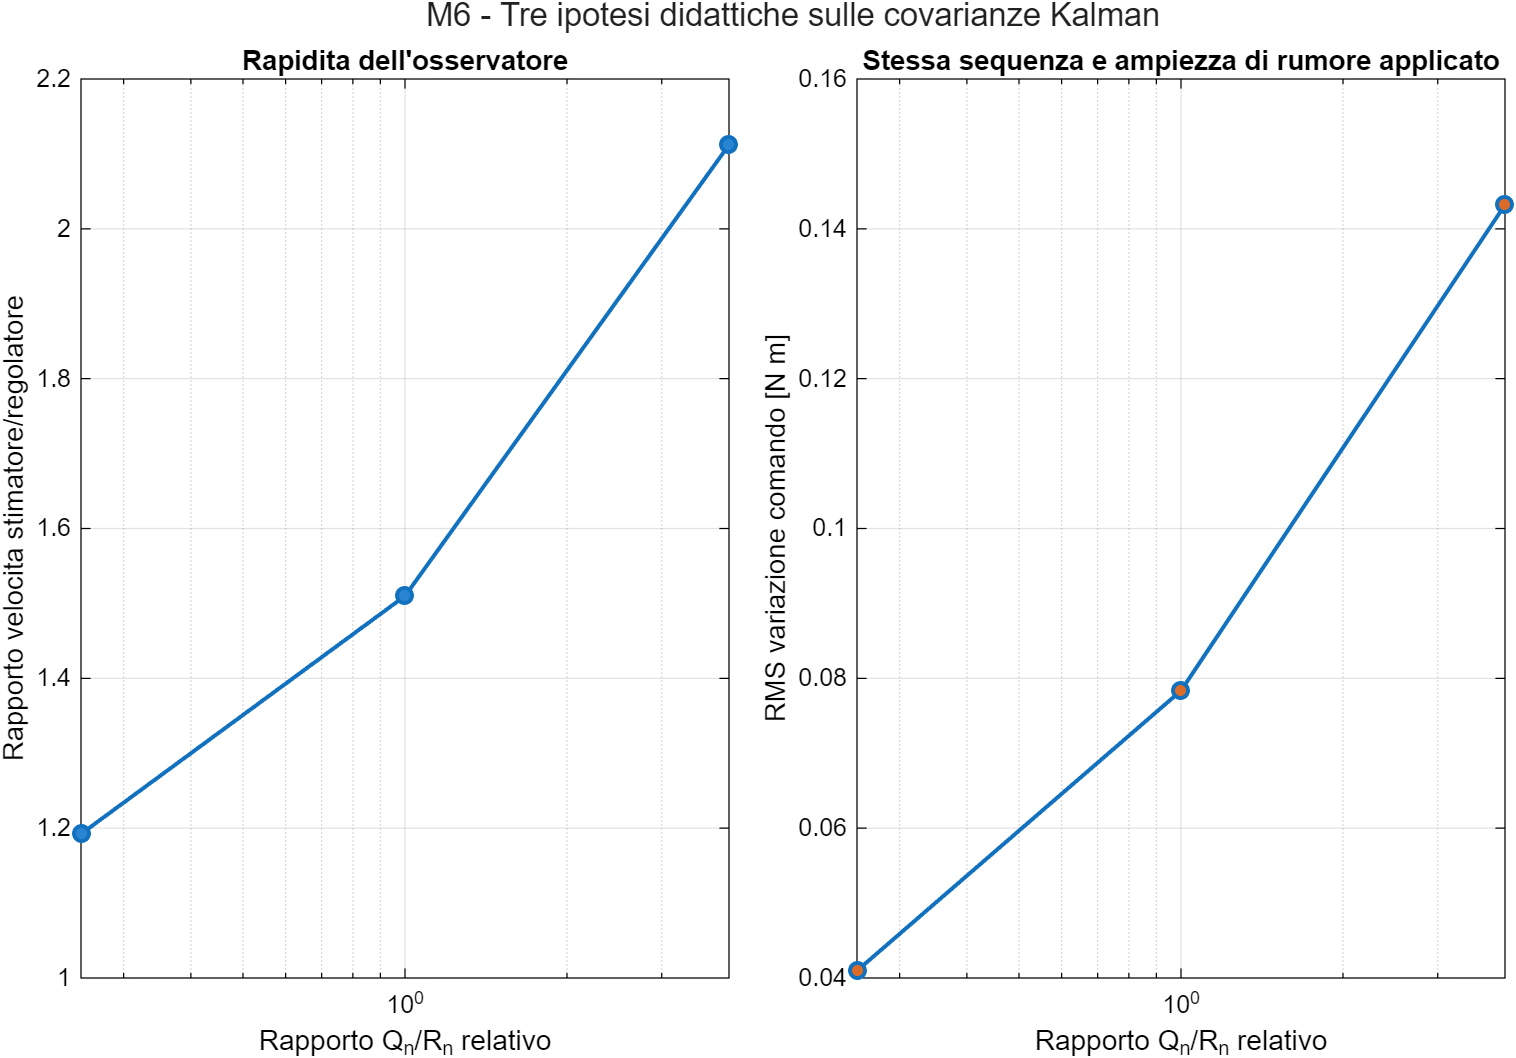
\includegraphics[width=0.84\textwidth]{figures/m6_kalman_sensitivity.png}
\caption{A sinistra, rapidità relativa dello stimatore; a destra, RMS della
variazione di coppia a rumore applicato identico. L'ascissa è il rapporto
$Q_n/R_n$ relativo al progetto nominale, non un rapporto adimensionale
fra grandezze fisiche eterogenee.}\label{fig:m6-kalman-sensitivity}
\end{figure}

\subsection{LQG e principio di separazione}
Per $z=[x^T,\hat x^T]^T$ la matrice completa è
\[
A_{cl}=\begin{bmatrix}A&-BK\\LC&A-BK-LC\end{bmatrix}.
\]
Con $e=x-\hat x$ si ottiene la forma triangolare
\[
\begin{bmatrix}\dot x\\\dot e\end{bmatrix}
=\begin{bmatrix}A-BK&BK\\0&A-LC\end{bmatrix}
\begin{bmatrix}x\\e\end{bmatrix}
\]
in assenza di ingressi esogeni. L'unione degli spettri di regolatore e stimatore
coincide quindi con quello della chiusura completa. La trasformazione viene
verificata numericamente nello script; il residuo è \RevSeparation.
Questo risultato riguarda stabilità nominale lineare, non robustezza rispetto
a M4 o stabilità non lineare globale.
\begin{table}[H]\centering\small
\begin{tabular}{rrrr}\toprule
$\Re\lambda(A-BK)$ & $\Im\lambda(A-BK)$ & $\Re\lambda(A-LC)$ & $\Im\lambda(A-LC)$ \\
\midrule
-6.17169 & 3.60433 & -9.31874 & 11.7171 \\
-6.17169 & -3.60433 & -9.31874 & -11.7171 \\
-11.8699 & 0 & -16.1307 & 78.1825 \\
-23.4741 & 86.4634 & -16.1307 & -78.1825 \\
-23.4741 & -86.4634 & -22.0159 & 84.7841 \\
-27.2576 & 43.8044 & -22.0159 & -84.7841 \\
-27.2576 & -43.8044 & -44.873 & 51.743 \\
-28.0575 & 84.428 & -44.873 & -51.743 \\
-28.0575 & -84.428 & -47.6737 & 29.4495 \\
-31.1221 & 0 & -47.6737 & -29.4495 \\
-52.8324 & 0 & -51.9324 & 32.5343 \\
-66.9325 & 0 & -51.9324 & -32.5343 \\
-133.333 & 0 & -133.333 & 0 \\
-133.333 & 0 & -133.333 & 0 \\
\bottomrule\end{tabular}
\caption{Poli in s$^{-1}$. Le due coppie di colonne elencano spettri distinti; le righe non associano un modo del regolatore a uno dello stimatore.}
\end{table}


\section{Risultati M6: lettura delle figure}
\subsection{Tracking del riferimento}
La Figura~\ref{fig:m6-tracking} usa tempo in secondi e deviazioni articolari
in gradi. Nel pannello superiore si applica $r_1=5^\circ,r_2=0$;
in quello inferiore $r_1=0,r_2=5^\circ$. Stato fisico e osservatore partono
da zero; coppie di disturbo e rumore sono nulli.
Le curve continue sono $q_1,q_2$, la tratteggiata il riferimento non nullo.
Si osservano rapidità del giunto comandato, picco del giunto non comandato e
raggiungimento del valore finale. Il peggiore $T_s$ è \MControllerWorstTs\ s:
M6 soddisfa i target nominali, pur senza disaccoppiamento perfetto.
\begin{figure}[H]\centering
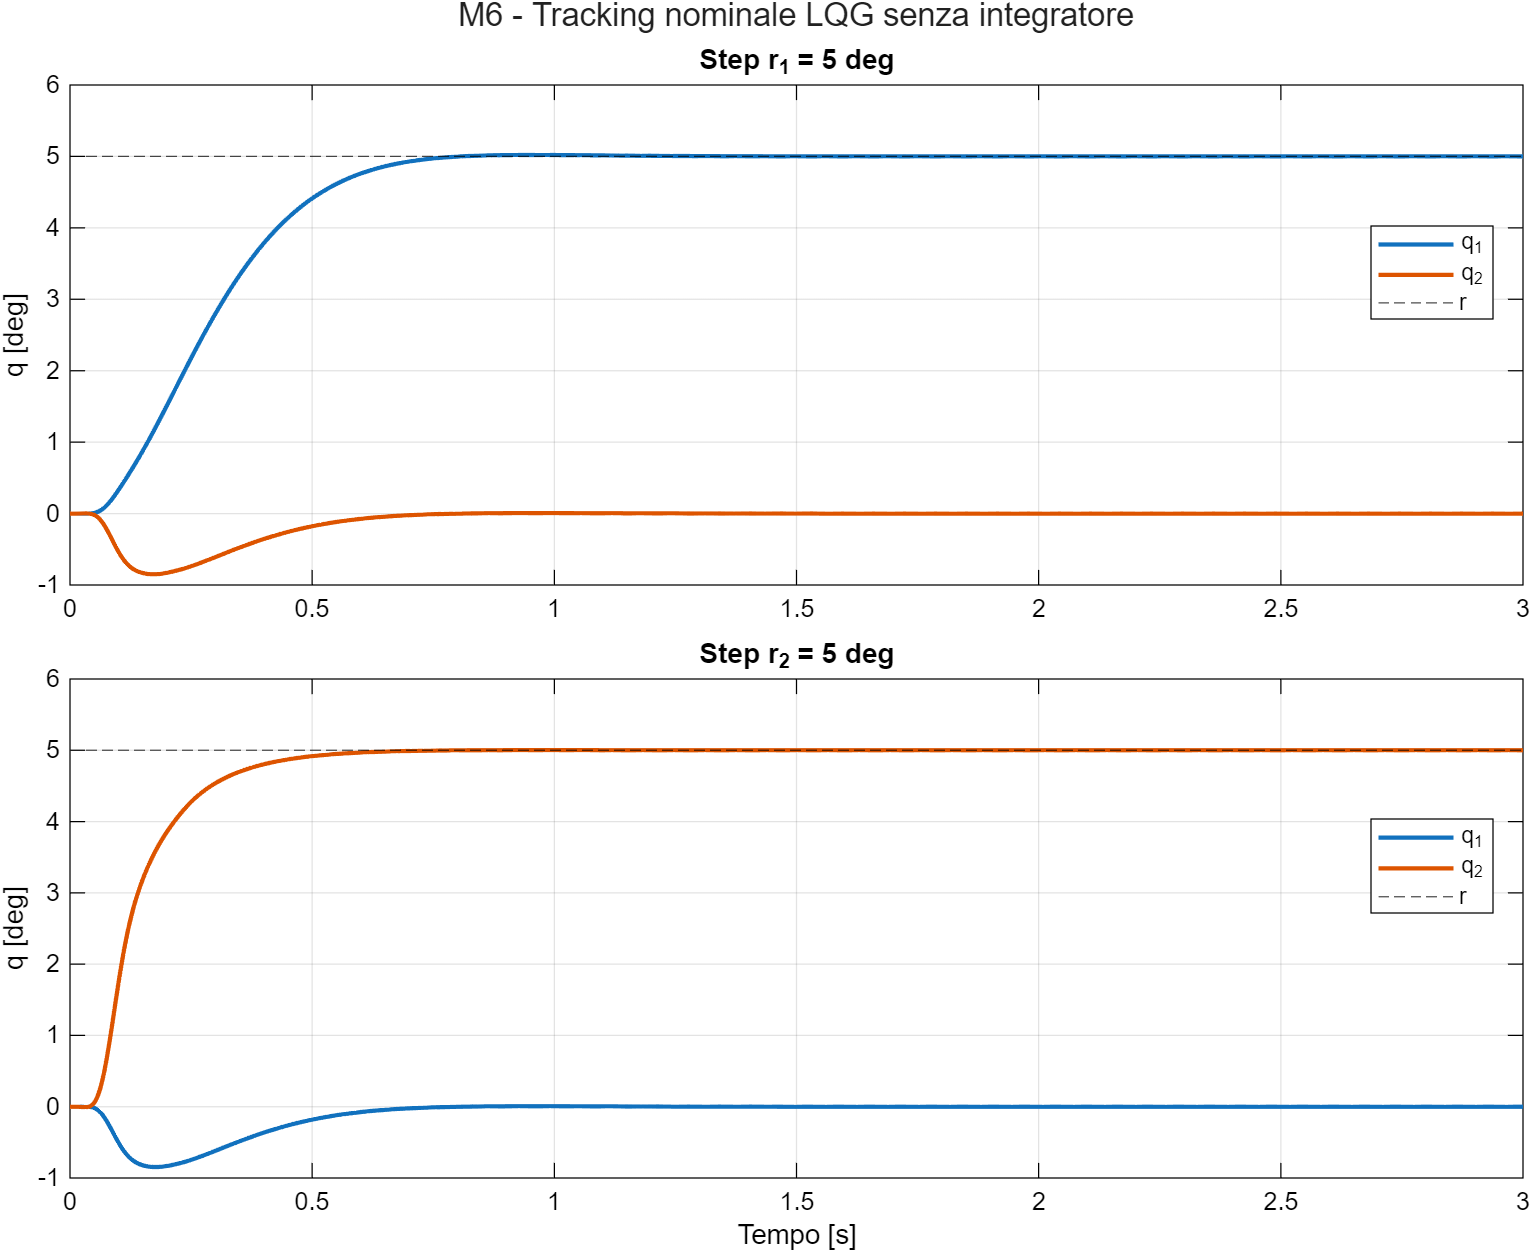
\includegraphics[width=0.82\textwidth]{figures/m6_lqg_reference_tracking.png}
\caption{Due prove di tracking nominale LQG a gradino di 5 gradi, senza disturbi
o rumore e da condizioni iniziali nulle.}\label{fig:m6-tracking}
\end{figure}

\subsection{Disturbo costante e limite del prefiltro}
Nella Figura~\ref{fig:m6-disturbo} il riferimento è nullo e si applica da $t=0$
una coppia costante di 0.5 N m al primo link (sopra) o al secondo (sotto).
Il rumore è nullo e gli stati iniziali sono nulli. Le curve riportano le due
deviazioni di posizione in gradi nel tempo. L'offset non nullo non è un errore
del grafico: il prefiltro corregge il guadagno statico sul riferimento,
non introduce l'azione integrale necessaria alla reiezione esatta.
\begin{figure}[H]\centering
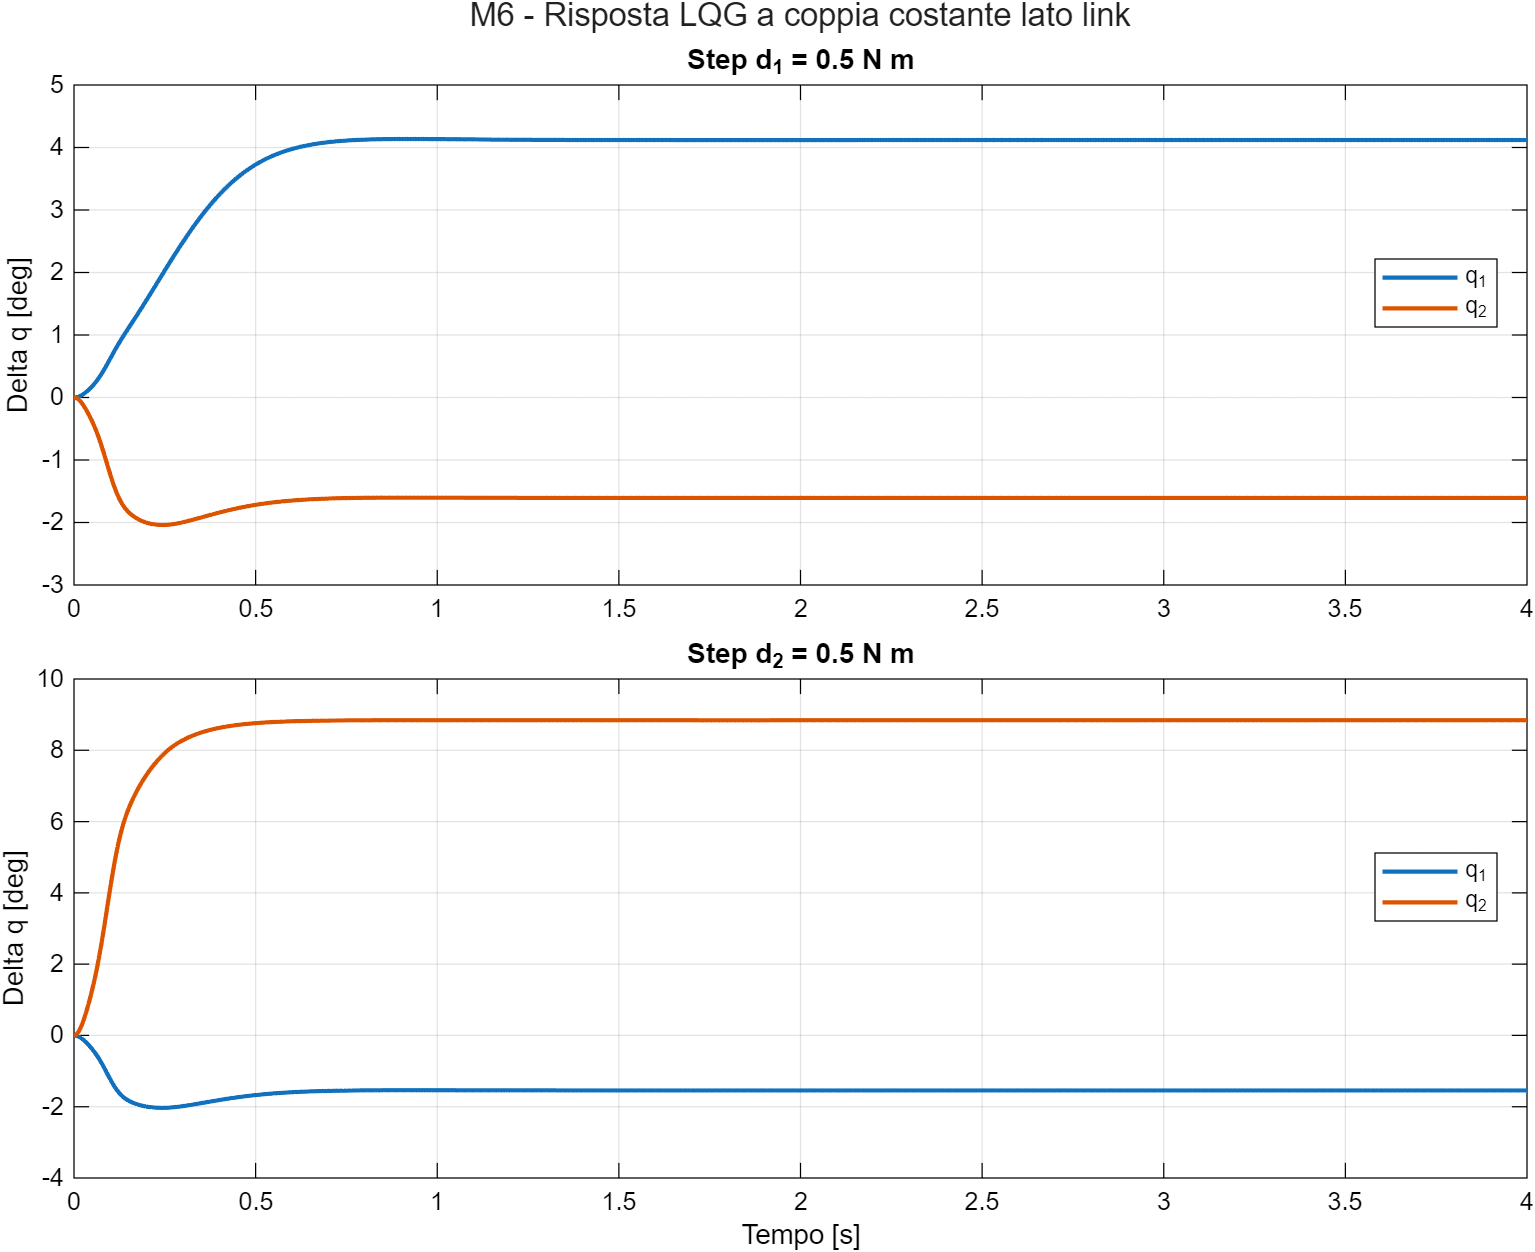
\includegraphics[width=0.82\textwidth]{figures/m6_lqg_disturbance_response.png}
\caption{Risposta ai due gradini di coppia lato link: il recupero resta stabile,
ma permane un offset coerente con l'assenza di integratori.}\label{fig:m6-disturbo}
\end{figure}

\subsection{Errore di stima e rumore sul comando}
La Figura~\ref{fig:m6-stima} usa lo scenario seeded di 4 s:
$r_1=5^\circ,r_2=0$, nessuna coppia disturbante, stati iniziali nulli
e rumore sui quattro encoder di deviazione standard 0.05 gradi.
Sopra si leggono $q_i-\hat q_i$ in gradi; sotto la differenza fra le coppie
della prova rumorosa e quelle della stessa prova senza rumore, in N m.
Non è quindi il comando totale. Le oscillazioni residue quantificano il
compromesso fra inseguimento delle misure e filtraggio.
\begin{figure}[H]\centering
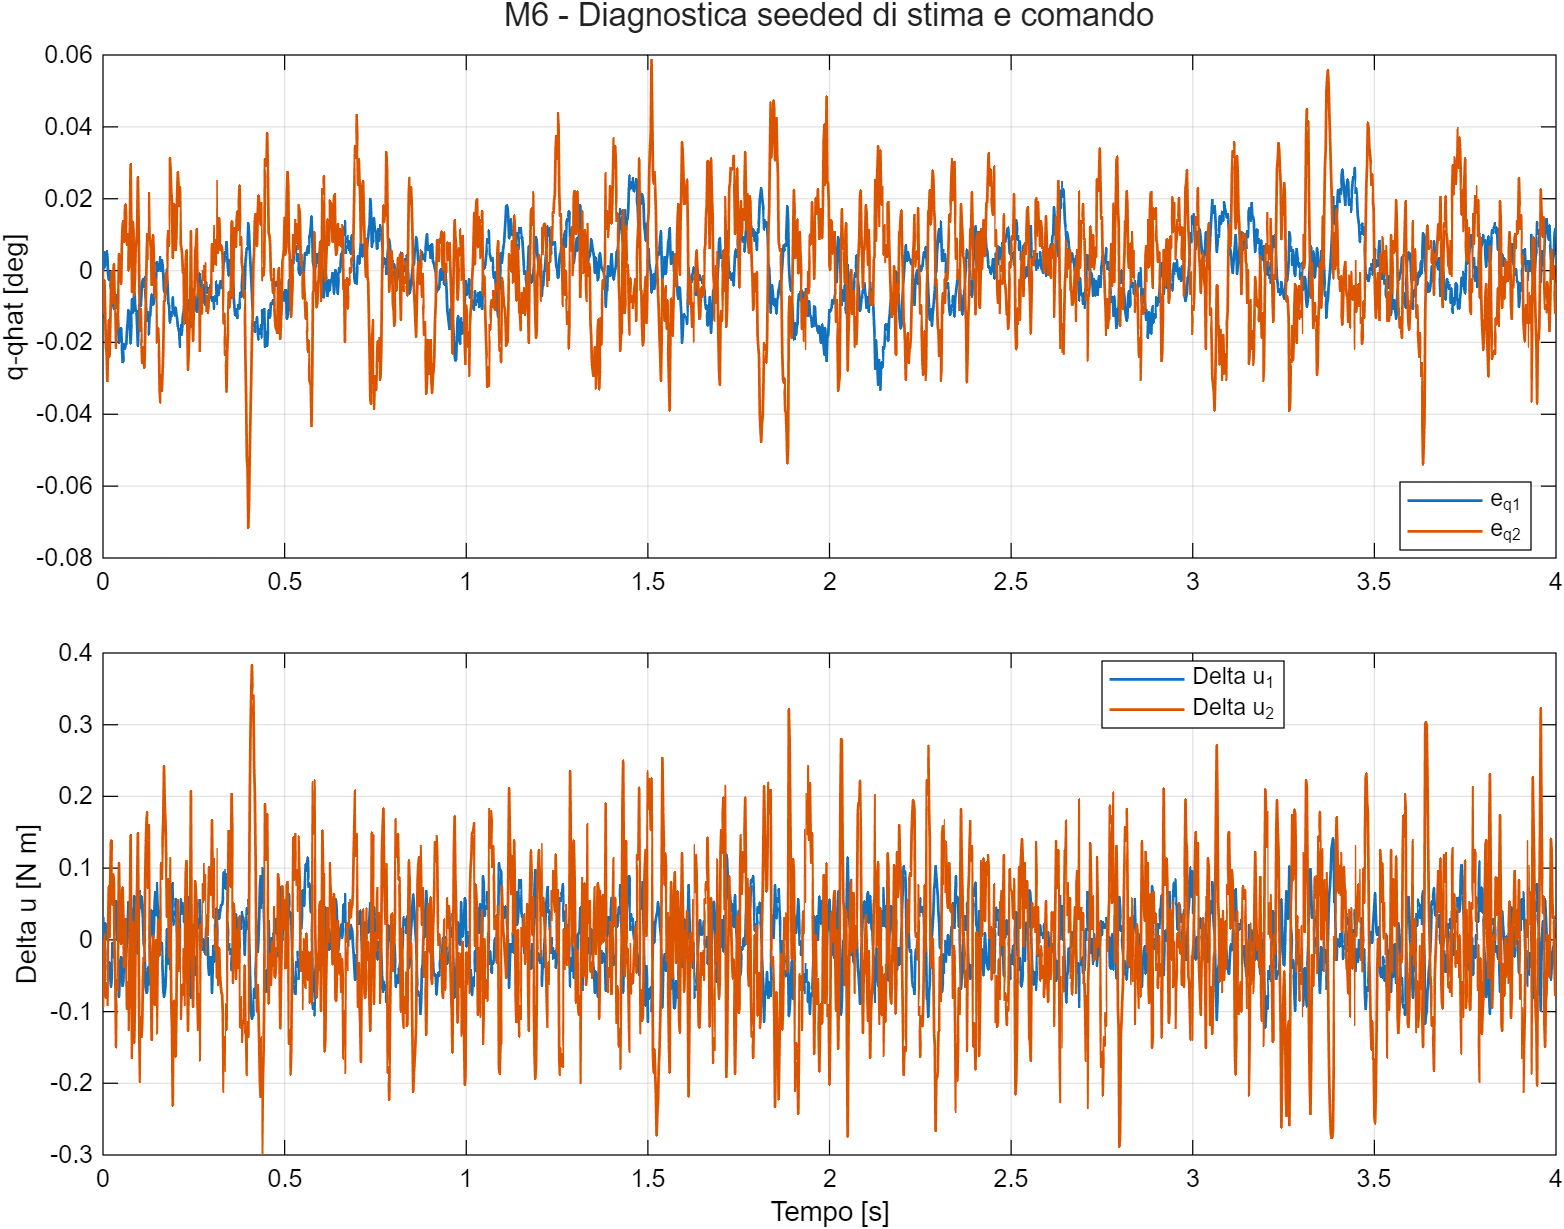
\includegraphics[width=0.82\textwidth]{figures/m6_lqg_estimation.png}
\caption{Errore sui due stati di posizione stimati e incremento di coppia
imputabile alla sequenza di rumore encoder, a riferimento identico.}\label{fig:m6-stima}
\end{figure}

\subsection{Poli e portata delle conclusioni}
La Figura~\ref{fig:m6-poli} non è una simulazione temporale: ascisse e ordinate
sono le parti reale e immaginaria dei poli in s$^{-1}$.
Non richiede condizioni iniziali, riferimenti o disturbi.
I simboli separano regolatore, stimatore e chiusura aumentata; la sovrapposizione
verifica il principio di separazione e la posizione a sinistra dell'asse
immaginario verifica la stabilità nominale.
\begin{figure}[H]\centering
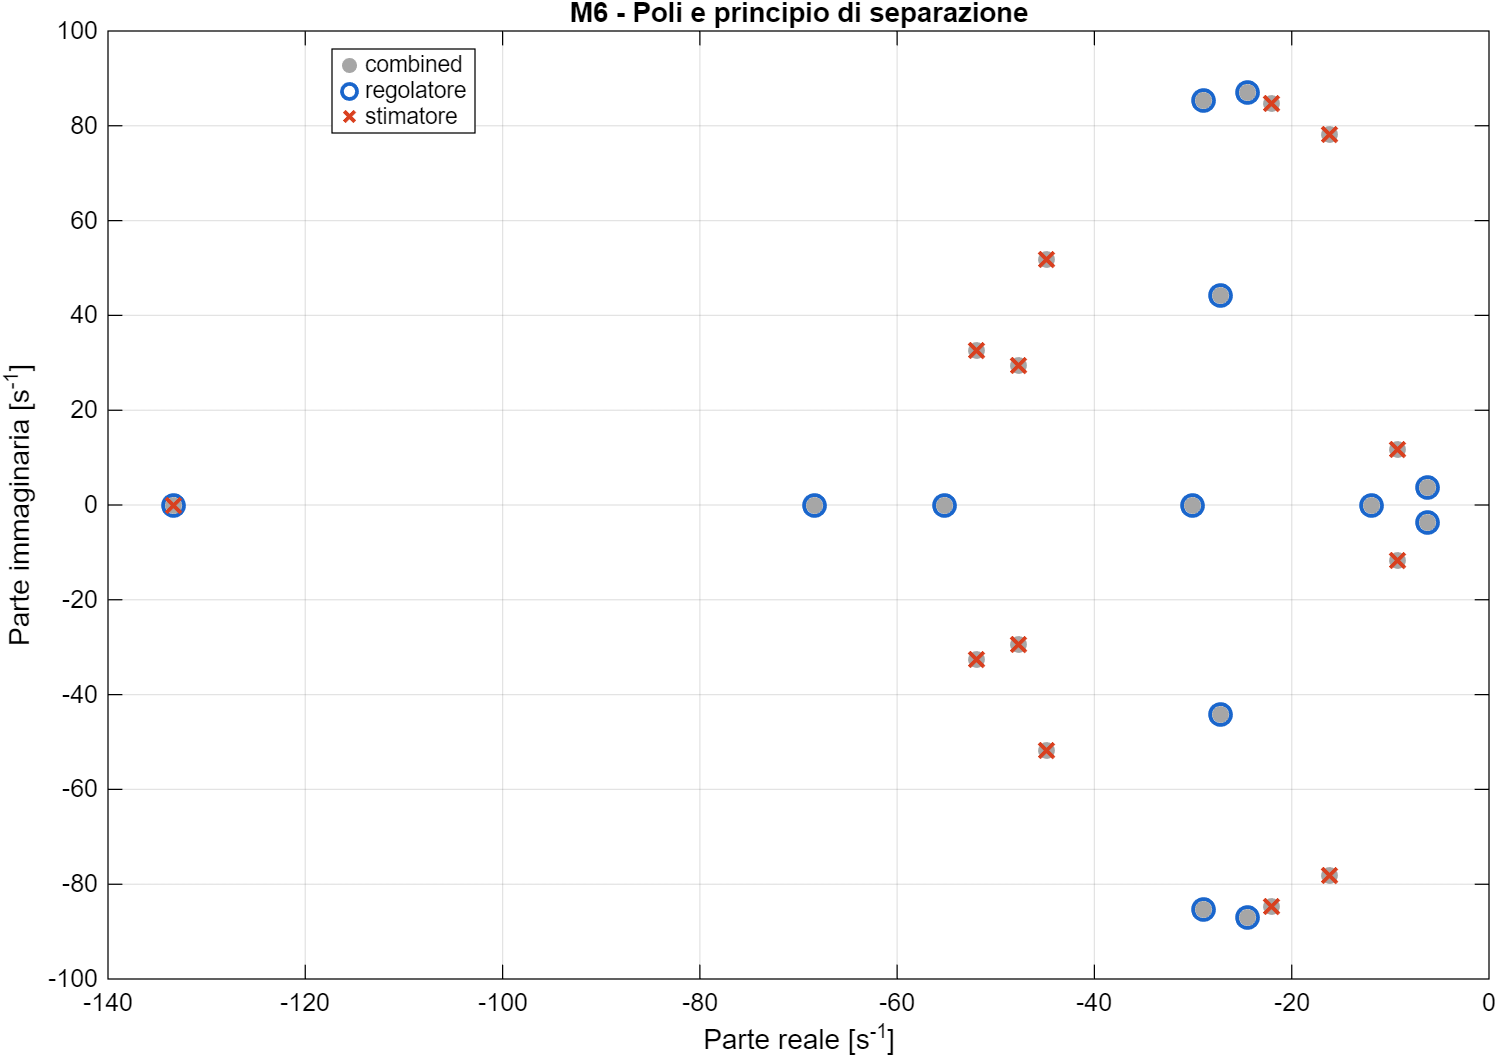
\includegraphics[width=0.80\textwidth]{figures/m6_lqg_poles.png}
\caption{Spettri del regolatore, dello stimatore e della chiusura LQG completa,
senza cancellazioni di stati.}\label{fig:m6-poli}
\end{figure}
Il comando full-state usato nella selezione ha picco peggiore
\MLqrPeakControl\ N m e RMS \MLqrRmsControl\ N m.
La verifica non lineare e il limite interno di Lyapunov, che includono
l'osservatore, sono sviluppati nel Capitolo 10; non sono dedotti dai soli poli.

\section{Implementazione Simulink didattica}
Il modello \texttt{SEA\_LQG\_nonlinear.slx} mostra al livello superiore sei blocchi funzionali: riferimento, controllore LQG, dinamica degli attuatori, pianta SEA non lineare, interfaccia di misura e monitoraggio. Dentro il controllore sono separati il prefiltro $N_r$, il feedback $-K\hat x$, la somma che genera il comando incrementale e l'osservatore di Kalman. Quest'ultimo realizza
\[
\dot{\hat x}=(A-LC)\hat x+B\,\delta u+L\,\delta y,
\qquad \delta u=-K\hat x+N_rr.
\]
L'interfaccia di misura estrae soltanto $q$ e $\theta$, sottrae l'equilibrio e aggiunge il rumore encoder; le velocità non vengono misurate. La coppia assoluta inviata agli attuatori è $u_{abs}=\bar\tau+\delta u$. Tutti i guadagni sono incorporati dall'artifact M6 validato e le condizioni iniziali vengono passate con \texttt{SimulationInput}; il modello non dipende dal base workspace. Non sono presenti saturazioni.

\section{Azione integrale e verifica LQI M7}
\label{sec:lqi}
\subsection{Dall'offset alla memoria dell'errore}
Le simulazioni precedenti mostrano il limite del solo prefiltro. La legge
$\delta u=-K\hat x+N_rr$ corregge il guadagno statico nominale da riferimento
a posizione, ma $N_r$ moltiplica soltanto $r$: non riceve l'errore prodotto
da una coppia disturbante. A riferimento nullo il suo contributo è nullo,
anche se $q$ converge a una posizione diversa dall'equilibrio.

Per le due posizioni articolari incrementali definiamo
\[
e(t)=r(t)-q(t)=r(t)-C_qx(t),\qquad
\xi(t)=\int_0^t e(\tau)\,d\tau,\qquad \dot\xi=r-C_qx,\quad \xi(0)=0.
\]
Ogni componente di $\xi$ è misurata in rad\,s. Un errore positivo fa crescere
la corrispondente componente; uno negativo la fa diminuire. Se l'errore
persiste, il suo integrale continua ad accumularsi: il regolatore dispone
così di una memoria del disallineamento. Un offset costante non può essere
compatibile con un equilibrio finito dell'intero sistema, perché in un
equilibrio deve essere anche $\dot\xi=0$.

Questa è l'applicazione del principio del modello interno ai segnali
costanti: si inseriscono due modi integrali, uno per uscita regolata.
Se la chiusura aumentata è stabile, ammette l'equilibrio richiesto e il
comando non è limitato da saturazioni, il regime costante ha $q=r$.
La correzione $-K_i\xi$ può restare non nulla anche dopo che $e$ si è
annullato: è proprio il contributo permanente necessario a bilanciare
il disturbo. Non si afferma invece che l'errore sia nullo durante il
transitorio o che il risultato valga automaticamente per il sistema incerto.

\subsection{Il sistema aumentato effettivo: 14 più 2 stati}
La pianta è ancora M3, con $A\in\mathbb R^{14\times14}$,
$B\in\mathbb R^{14\times2}$ e $C_q\in\mathbb R^{2\times14}$.
Lo stato $x$ comprende gli otto stati meccanici e i sei stati attuativi
già descritti; non vengono eliminati gli attuatori. Ponendo
$x_a=[x^T,\xi^T]^T\in\mathbb R^{16}$ si ottiene
\[
\begin{bmatrix}\dot x\\\dot\xi\end{bmatrix}
=
\underbrace{\begin{bmatrix}A&0_{14\times2}\\-C_q&0_{2\times2}\end{bmatrix}}_{A_a}
\begin{bmatrix}x\\\xi\end{bmatrix}
+\underbrace{\begin{bmatrix}B\\0_{2\times2}\end{bmatrix}}_{B_a}u
+\underbrace{\begin{bmatrix}0_{14\times2}\\I_2\end{bmatrix}}_{B_r}r.
\]
Il disturbo lato link aggiunge $B_{d,a}d$, con
$B_{d,a}=[B_d^T,0_{2\times2}]^T$. Le dimensioni di $A_a,B_a,B_r$
sono rispettivamente $16\times16$, $16\times2$, $16\times2$.

L'aggiunta degli integratori non è innocua: se un modo non stabile non
è controllabile, Riccati non può fornire un regolatore stabilizzante.
Il costruttore \texttt{build\_lqi\_augmented\_cost.m} verifica
\[
\operatorname{rank}\,[\lambda I_{16}-A_a\;\;B_a]=16
\quad\text{per i poli con }\Re\lambda\geq-10^{-8}.
\]
Il test PBH all'origine restituisce 16, come il rango della matrice
di Rosenbrock
\[
\operatorname{rank}\begin{bmatrix}A&B\\C_q&0\end{bmatrix}=16.
\]
Non vi è quindi un'ostruzione dovuta a zeri invarianti nell'origine.
Questi controlli sono preferibili a interpretare ingenuamente il solo
rango numerico di \texttt{ctrb}, sensibile allo scaling e alle potenze di $A_a$.

\subsection{Costo, scala integrale e significato di \texorpdfstring{$w_i$}{wi}}
Il problema risolto è
\[
J_{\rm LQI}=\int_0^\infty
\left(x^TQx+\xi^TQ_i\xi+u^TRu\right)dt
=\int_0^\infty\left(x_a^TQ_ax_a+u^TRu\right)dt,
\qquad Q_a=\operatorname{blkdiag}(Q,Q_i).
\]
Il blocco $Q$ è esattamente quello M6, inclusi i termini non diagonali.
Il codice adotta
\[
s_\xi=q_sT_{s,\mathrm{target}}
=(5\pi/180)\,0.8\ {\rm rad\,s},\qquad
Q_i=\frac{w_i}{s_\xi^2}I_2,\qquad
R=\frac{\rho_U}{u_{\mathrm{scale}}^2}I_2.
\]
La scala $s_\xi$ è derivata dai target progettuali M5: rappresenta
l'accumulo di un errore pari a $q_s$ per un tempo pari al settling richiesto.
Non è una misura sperimentale né un limite fisico dell'integratore.
Invece $w_i$ è una priorità adimensionale di tuning: pesa
$\|\xi/s_\xi\|^2$ nel costo, senza cambiare la scala o il requisito M5.

Con $w_i$ piccolo l'accumulo costa relativamente poco; con $w_i$ grande
il problema LQR tende a contrastarlo maggiormente. Ci si attende in genere
una correzione integrale più rapida, ma anche possibili aumenti di
sovraelongazione e comando. Non è una monotonicità garantita per qualsiasi
sistema MIMO. Non esiste pertanto un unico $w_i$ teoricamente corretto:
dipende dal compromesso che si intende studiare.

I tre casi originali sono $(w_i,\rho_U)=(0.1,16),(1,8),(4,4)$,
denominati debole, intermedio e forte. Non sono tre prove a parità di $R$:
all'aumento di $w_i$ si accompagna una riduzione della penalizzazione
del comando. Non si può attribuire l'intera variazione delle prestazioni
al solo integratore. Una verifica diagnostica aggiuntiva mantiene invece
$\rho_U=16$ e lo stesso $Q$: per $w_i=0.1,1,4$ si ottengono
$\|K_i\|_2=13.589,\ 42.972,\ 85.944$ e parti reali dominanti
$-0.2610,\ -0.8307,\ -1.6975$ s$^{-1}$. In queste tre prove l'azione
integrale cresce e il modo lento accelera; i punti originali M7 non
vengono sostituiti né viene effettuata una nuova selezione del controllore.

\subsection{Da Riccati a \texorpdfstring{$K_x$ e $K_i$}{Kx e Ki}: convenzione di segno}
Fissati $Q,Q_i,R$, MATLAB risolve
\[
A_a^TP_a+P_aA_a-P_aB_aR^{-1}B_a^TP_a+Q_a=0,
\qquad
K_a=R^{-1}B_a^TP_a=[K_x\;\;K_i].
\]
La chiamata è \texttt{[Kaug,Pa,poli]=lqr(Aaug,Baug,Qaug,R)}:
$K_a$ ha dimensione $2\times16$, $K_x$ è $2\times14$ e $K_i$ è
$2\times2$. $K_i$ non è scelto a mano. La catena è
\[
Q,Q_i,R\ \longrightarrow\ Q_a\ \longrightarrow\ P_a\
\longrightarrow\ K_a\ \longrightarrow\ (K_x,K_i).
\]
Con $\dot\xi=r-q$ la legge effettiva M7 è
\[
u=-K_xx-K_i\xi+N_{ff}r,\qquad
N_{ff}=[-C_q(A-BK_x)^{-1}B]^{-1}.
\]
Il prefiltro è ricalcolato da $K_x$, non copiato da M6.
Nel punto intermedio le diagonali di $K_i$ sono negative: il meno
davanti a $K_i\xi$ non va cancellato o reinterpretato. La sua correttezza
è verificata dalla matrice chiusa
\[
A_{\rm LQI}=
\begin{bmatrix}A-BK_x&-BK_i\\-C_q&0\end{bmatrix}
\]
e dall'annullamento della mappa statica $d\mapsto q$.
Per il solo confronto illustrativo si usa il punto intermedio,
$w_i=1,\rho_U=8$, senza promuoverlo a soluzione finale.
Le matrici seguenti e i residui sono esportati dallo script eseguito.
% Generated by plot_lqi_hinf_revision.m.
\[
Q_i=205.18I_2,\qquad R=0.055556I_2,\qquad s_\xi=0.069813\ {\rm rad\,s}.
\]
\[
K_x=[K_{x,a}\ K_{x,b}],\quad K_{x,a}=K_x(:,1{:}7),\quad K_{x,b}=K_x(:,8{:}14).
\]
\[K_{x,a}=\begin{bmatrix}
381.75 & 24.782 & 25.889 & 5.3979 & -248.18 & -18.735 & -1.2107 \\
22.296 & 307.95 & 6.735 & 9.553 & -6.014 & -205.35 & -0.88562 \\
\end{bmatrix}.\]
\[K_{x,b}=\begin{bmatrix}
-1.2396 & 13.998 & 27.737 & 61.323 & -1.0238 & -2.6308 & -16.996 \\
2.3461 & -1.0238 & -2.4981 & -13.938 & 16.824 & 34.815 & 108.21 \\
\end{bmatrix}.\]
\[K_i=\begin{bmatrix}
-60.707 & 2.7917 \\
-2.7917 & -60.707 \\
\end{bmatrix}.\]
\[N_{ff}=\begin{bmatrix}
89.441 & 0.45133 \\
8.1751 & 78.52 \\
\end{bmatrix}.\]
Il residuo relativo dell'ARE è $\num{1.2858e-13}$; $\|K_a-R^{-1}B_a^TP_a\|_F=\num{1.8532e-11}$.
\begin{table}[htbp]\centering\small
\begin{tabular}{rrrrrr}\toprule
$w_i$ & $\rho_U$ & $\|K_i\|_2$ & $T_s$ [s] & OS [\%] & picco $u$ [N m] \\\midrule
0.1 & 16 & 13.589 & \(\infty\) & 7.1007 & 4.8589 \\
1 & 8 & 60.771 & \(\infty\) & 16.585 & 7.8052 \\
4 & 4 & 171.89 & 2.168 & 25.047 & 12.921 \\
\bottomrule\end{tabular}
\caption{Tre punti M7 originali, tracking a 5 gradi su 3 s. $\infty$ significa mancato assestamento entro l'orizzonte, non instabilità.}
\label{tab:lqi-tre-punti}\end{table}
\begin{table}[htbp]\centering\small
\begin{tabular}{llrrrr}\toprule
Controllo & Disturbo & $q_1(\infty)$ & $q_2(\infty)$ & picco $u$ & RMS $u$ \\\midrule
LQG & $d_1$ & 4.1497 & -1.6254 & 1.2932 & 0.7874 \\
LQG & $d_2$ & -1.5621 & 8.9306 & 1.1591 & 0.57365 \\
LQI & $d_1$ & 0 & 0 & 0.87156 & 0.39352 \\
LQI & $d_2$ & 0 & 0 & 1.1324 & 0.37559 \\
\bottomrule\end{tabular}
\caption{Disturbi da 0.5 N m, posizioni asintotiche in gradi e coppie in N m. RMS calcolato su entrambi i comandi negli stessi 8 s.}
\label{tab:lqi-disturbo-numeri}\end{table}


\subsection{Confronto corretto: LQG stimato e LQI a stato vero}
Il confronto non riguarda due architetture con gli stessi sensori.
M6 usa $\hat x$ stimato da $q,\theta$; la verifica M7 usa $x$ vero.
Il sistema chiuso LQG ha 28 stati, mentre il servo LQI ideale ne ha 16.
L'integratore è un'estensione del problema di regolazione, non la
presenza implicita di un filtro Kalman. Un'implementazione sullo stato
stimato richiederebbe esplicitamente $u=-K_x\hat x-K_i\xi+N_{ff}r$
e una nuova verifica della chiusura completa, non effettuata qui.

\begin{table}[H]\centering\small
\begin{tabular}{p{2.7cm}p{5.5cm}p{5.5cm}}\toprule
Aspetto & LQG M6 & LQI M7 illustrativo \\\midrule
Feedback e stato & $-K\hat x+N_rr$; stima Kalman & $-K_xx-K_i\xi+N_{ff}r$; stato vero \\
Memoria dell'errore & Nessun integratore di $r-q$ & Due stati $\xi$ in rad\,s \\
Tracking nominale & Guadagno statico unitario con prefiltro & Guadagno statico unitario nella chiusura stabile \\
Disturbo costante & Offset generalmente non nullo & Offset asintotico nullo nelle prove nominali \\
Complessità & 14 stati di osservatore, 28 chiusi & 2 integratori, 16 chiusi; stato vero richiesto \\
Overshoot e tuning & M6 soddisfa i target nominali & Dipendono da $Q_i,R$; nessun caso M7 rispetta tutti i target \\
Sforzo di controllo & Da valutare per lo scenario & Non cresce necessariamente in ogni prova; confrontare le metriche \\
Saturazioni & Assenti nel modello & Assenti; accumulo e windup possibili in un attuatore reale saturato \\
Vantaggio & Prestazione nominale con misure disponibili & Reiezione nominale dei disturbi costanti \\
Limite & Non elimina l'offset da coppia costante & Settling/overshoot non conformi; servirebbero stima e anti-windup in una realizzazione con saturazioni \\\bottomrule
\end{tabular}
\caption[Confronto delle architetture LQG e LQI]{Differenze fra le architetture effettivamente simulate, non proprietà universali delle sigle LQG e LQI.}
\label{tab:lqg-lqi-logica}
\end{table}

La Figura~\ref{fig:lqi-disturbo} applica due prove separate sul medesimo
modello nominale: $r=0$, condizioni iniziali nulle, nessun rumore,
disturbo a partire da $t=0$ e orizzonte comune di 8 s.
Le colonne distinguono $d=[0.5,0]^T$ e $d=[0,0.5]^T$ N m;
le righe mostrano $q_1$ e $q_2$ in gradi. Ogni asse sovrappone LQG e LQI.
L'offset LQG non è un transitorio incompleto: coincide con il guadagno DC.
LQI converge invece verso zero; a 8 s il massimo residuo osservato
è circa $8.73\cdot10^{-5}$ rad, distinto dallo zero asintotico calcolato.
La Figura~\ref{fig:lqi-comando} usa gli stessi esperimenti e mostra
le coppie incrementali. In queste prove LQI non richiede un picco maggiore
di M6: elimina l'offset con un contributo statico che bilancia la coppia
disturbante. Questo non contraddice i maggiori picchi osservati nel
tracking, che è uno scenario diverso.
\begin{figure}[!htbp]\centering
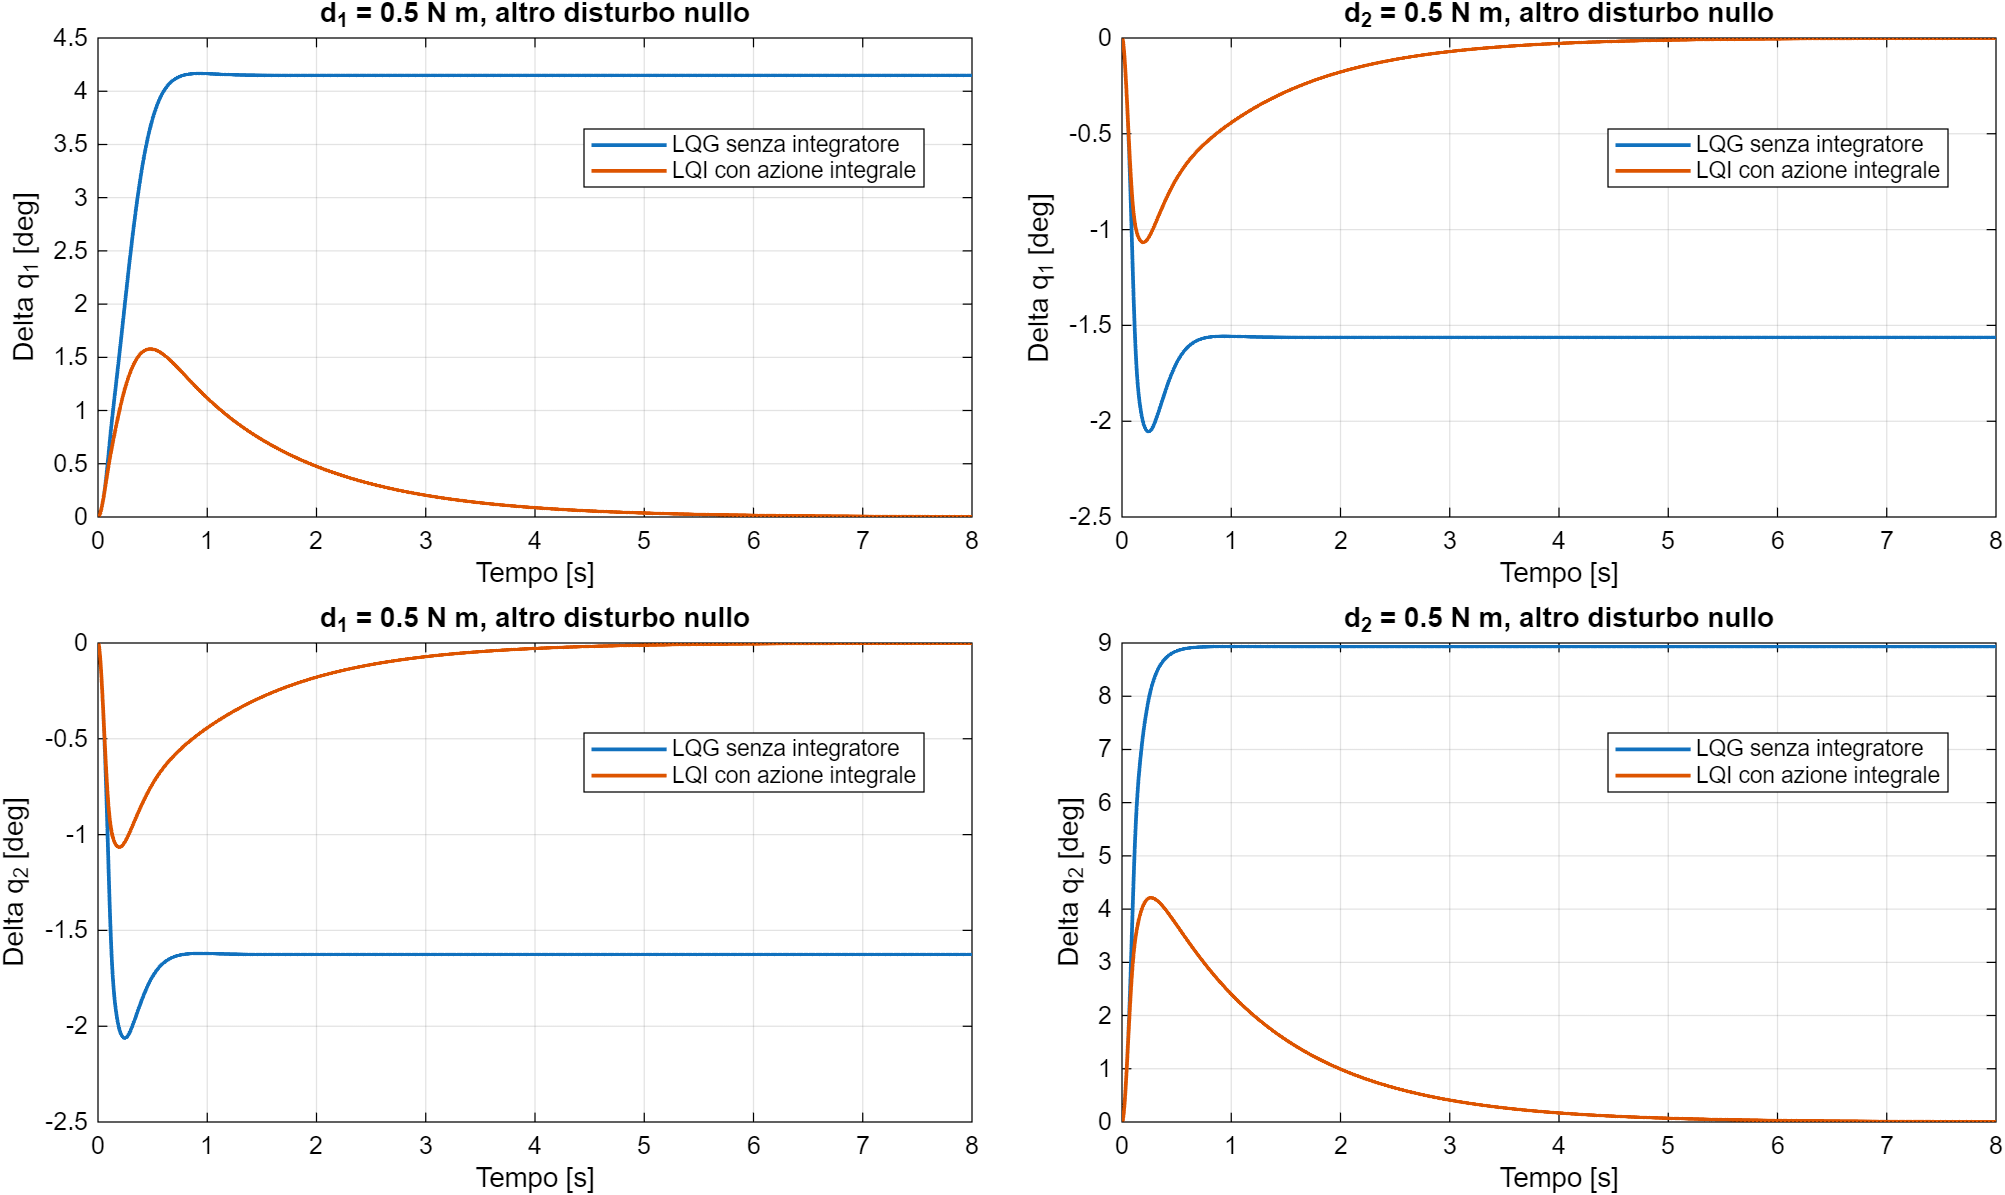
\includegraphics[width=0.86\textwidth]{figures/m7_lqg_lqi_constant_disturbance.png}
\caption{LQG senza integratore e LQI a stato vero, punto $(w_i,\rho_U)=(1,8)$, sotto le due coppie costanti da 0.5 N m. Tutti gli ingressi e gli stati iniziali sono identici; cambia l'architettura di feedback.}
\label{fig:lqi-disturbo}
\par\medskip
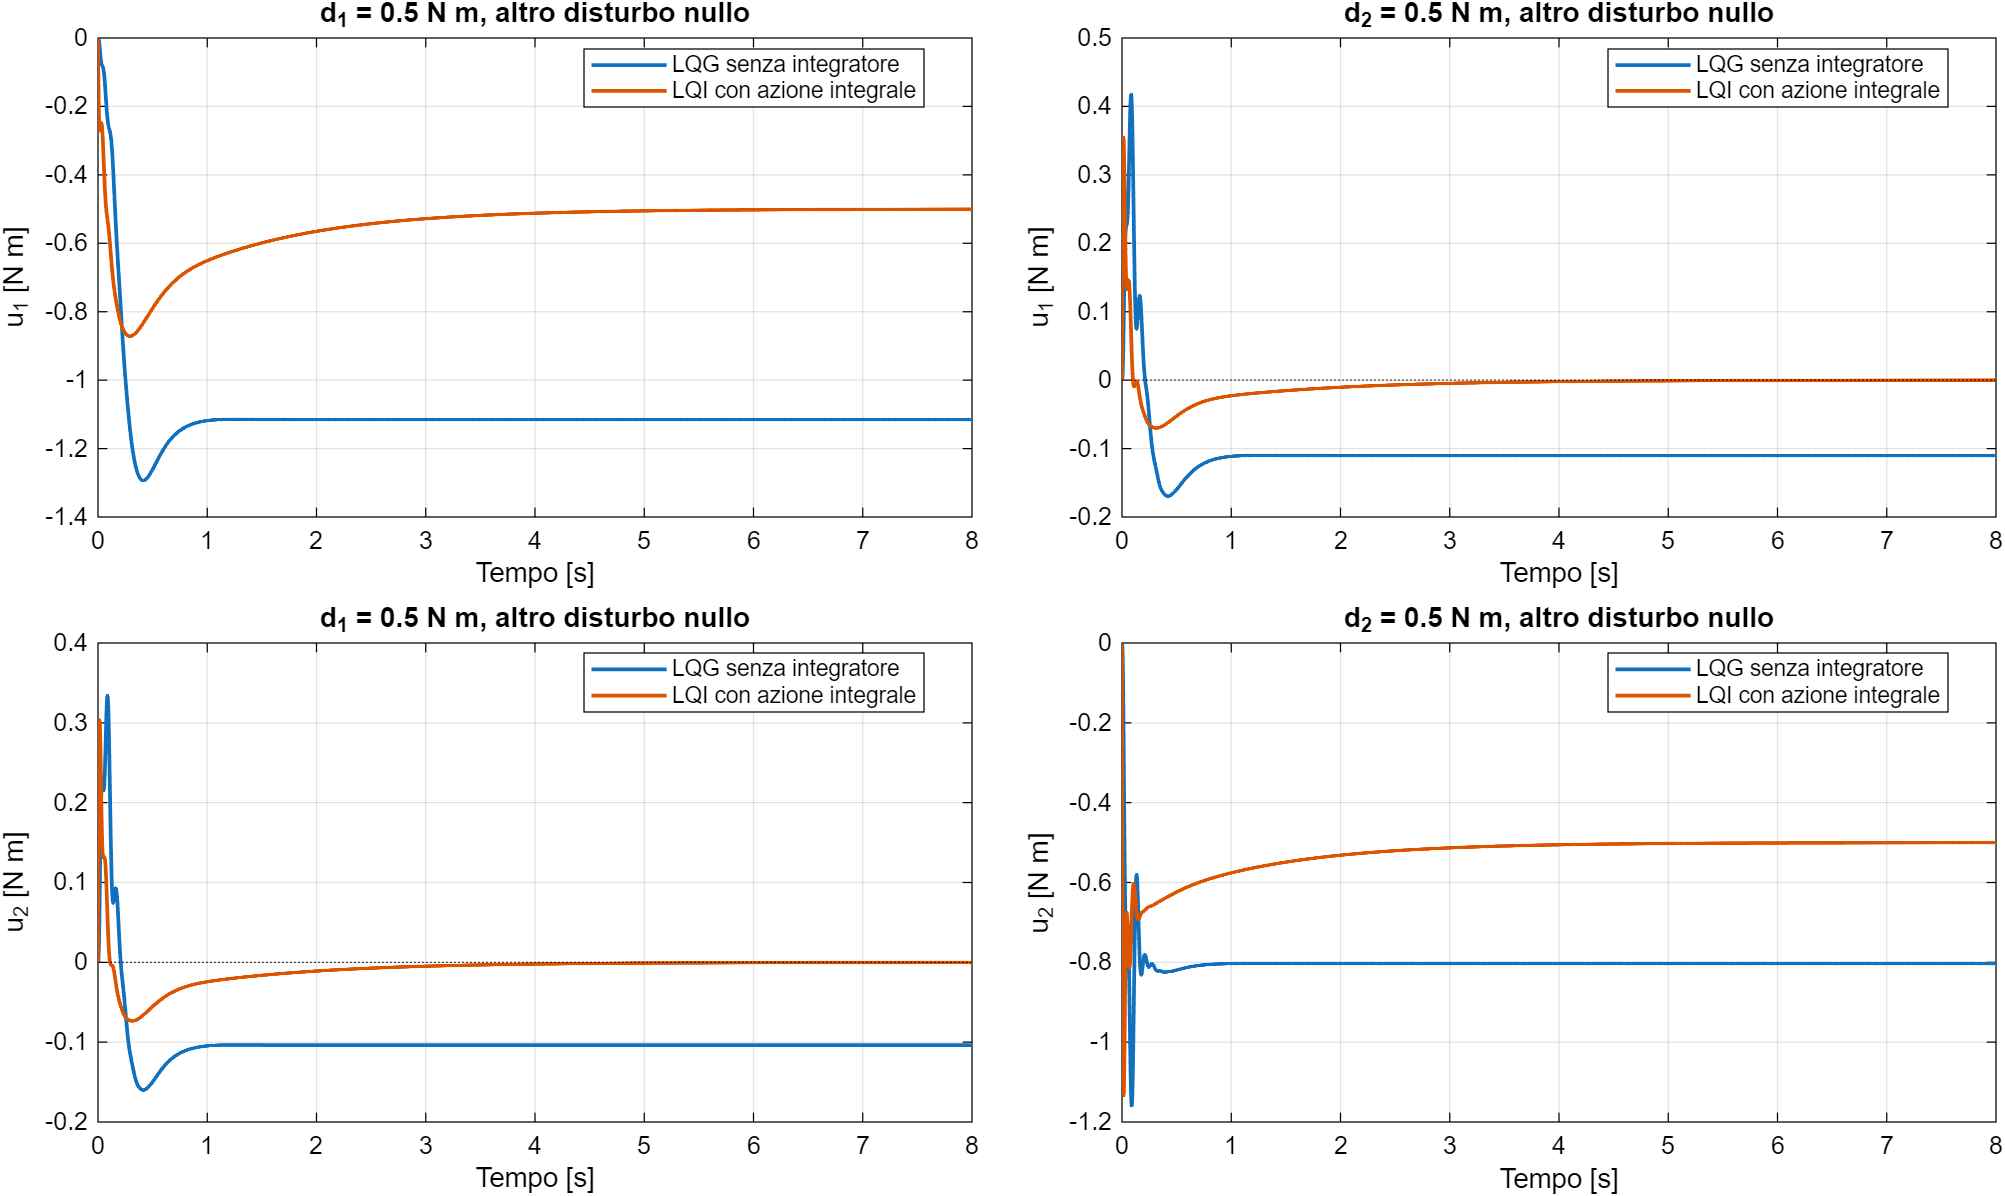
\includegraphics[width=0.86\textwidth]{figures/m7_lqg_lqi_disturbance_control.png}
\caption{Comandi degli stessi due esperimenti della Figura~\ref{fig:lqi-disturbo}. Non sono applicate saturazioni o compensazioni anti-windup.}
\label{fig:lqi-comando}
\end{figure}

\subsection{Perché lo studio non sostituisce il controllore nominale}
La Tabella~\ref{tab:lqi-tre-punti} conserva l'esito M7: tutti i punti sono
stabili e rigettano i disturbi costanti, ma i primi due non si assestano
entro 3 s e il terzo richiede $2.168$ s con overshoot $25.05\%$.
Il target M5 è $0.8$ s e $10\%$. Il punto intermedio usato nei grafici
ha overshoot $16.59\%$ e picco di tracking $7.805$ N m.
Il caso forte raggiunge $12.921$ N m: il superamento della scala
prestazionale di 12 N m non è una simulazione di saturazione hardware.

Se un attuatore reale saturasse, l'errore potrebbe continuare ad accumularsi
mentre il comando richiesto non è realizzabile: sarebbe necessaria una
strategia anti-windup, assente dal progetto. M7 resta dunque
\status{\MSevenStatus}, con \MSevenAdmissible\ punti conformi a tutti
i criteri. La reiezione dell'offset è un vantaggio reale, ma non basta
a sostituire M6 né a certificare robustezza.

\chapter{Controllo $H_\infty$: baseline e revisione mirata}
\label{cap:hinf}
\section{Obiettivo energetico e mappe della retroazione}
Il controllo $H_\infty$ cerca un regolatore che limiti il peggiore guadagno
delle mappe di interesse. Per una matrice di trasferimento stabile $F$,
\[
\|F\|_\infty=\sup_{\omega\in\mathbb R}\bar\sigma(F(j\omega))
=\sup_{0<\|w\|_2<\infty}\frac{\|z\|_2}{\|w\|_2},\qquad z=Fw.
\]
Si considera quindi la peggiore frequenza e la peggiore direzione MIMO
dell'ingresso, non la media dei due giunti. L'interpretazione energetica
riguarda ingressi a energia finita. Un gradino permanente non è in $L_2$:
settling, overshoot e picco istantaneo di coppia devono essere verificati
separatamente, non dedotti automaticamente dalla norma.

Per la pianta M3, $G:u\mapsto q$ ha dimensione $2\times2$, 14 stati,
ingressi in N m e uscite in rad. Il regolatore riceve $e=r-q$ e produce
$u=Ke$. Definiamo le mappe all'uscita
\[
S=(I+GK)^{-1},\qquad
T=GK(I+GK)^{-1}=I-S,\qquad
KS=K(I+GK)^{-1}.
\]
$S$ collega riferimento ed errore, $T$ riferimento e posizione,
$KS$ riferimento e comando. Un rumore additivo di misura si trasmette
alla posizione mediante $-T$ e al comando mediante $-KS$.
Per la coppia disturbante lato link, invece, la mappa fisica è
$SG_d$: non basta chiamare $S$ la risposta a qualsiasi disturbo.

LQG e $H_\infty$ rispondono a problemi diversi. M6 impiega una stima
dello stato basata su $q,\theta$ e ipotesi statistiche sui rumori;
la sintesi qui studiata utilizza soltanto i due errori di posizione $r-q$
e minimizza un criterio frequenziale worst-case. Non riutilizza $K$ o $L$
di M6 e non dispone automaticamente delle stesse prestazioni.

\section{Pesi originali M5: significato e audit delle unità}
La configurazione originaria usa
\[
W_1(s)=\frac{s/2+12}{s+0.6}I_2,\qquad
W_2(s)=\frac1{12}\frac{s/30+1}{s/180+1}I_2,\qquad W_3=\varnothing.
\]
$W_1(0)=20$ traduce l'obiettivo di sensibilità statica $A_s=0.05$;
$W_1(\infty)=0.5$ corrisponde al parametro $M_s=2$.
Il polo è $0.6$, lo zero $24$ e la frequenza $|W_1|=1$ è
$13.839$ rad/s: $\omega_B=12$ è un parametro di transizione,
non una misura della banda effettivamente ottenuta.
$W_2$ ha guadagno DC $1/12$, guadagno asintotico $0.5$,
zero $30$ e polo $180$ rad/s. Non attraversa il livello uno.

La simmetria dei due pesi è coerente con le medesime unità e scale
dei due giunti, ma non rende isotropa la pianta: a 12 rad/s i valori
singolari di $G$ sono circa $0.1713$ e $0.0101$ rad/(N m).
La direzione meno controllabile in frequenza richiede un comando
molto maggiore a parità di uscita.

Il prodotto $W_2KS$ della baseline agisce sul guadagno da un riferimento
espresso numericamente in rad al comando. Non impone direttamente
$|u(t)|\leq12$ N m per il gradino di 5 gradi.
La scala di riferimento implicita è 1 rad, non $q_s=5\pi/180$ rad.
Questo non rende falso il vecchio problema matematico: ne rende il costo
di comando più restrittivo rispetto a un problema esplicitamente
normalizzato sul caso M5 da 5 gradi. Correggere l'interpretazione delle
unità non autorizza a presentare una norma $L_2$ come limite di picco.

Anche la traduzione temporale è una scelta di loop shaping, non
un'equivalenza: imporre un inviluppo su $S$ con $A_s,M_s,\omega_B$
non garantisce da solo $T_s\leq0.8$ s e overshoot $\leq10\%$.
Il modello comprende inoltre poli instabili a circa $4.0408$ e
$7.2094$ s$^{-1}$, dinamica attuativa con $\omega_n=40$ rad/s,
ritardo nominale 15 ms e due zeri di Padé nel semipiano destro
a $133.333$ s$^{-1}$. Questi elementi vincolano la stabilizzazione
e il compromesso di banda; non sono eliminati dalla normalizzazione.

\subsection{Una incompatibilità verificabile prima del retuning}
Con pesi scalari replicati sui due giunti, poniamo
$a=|W_{1,\mathrm{siso}}(j\omega)|$,
$b=|W_{2,\mathrm{siso}}(j\omega)|$ e
$g=\underline\sigma(G(j\omega))$. Poiché $S+GKS=I$, persino
rilassando il problema e scegliendo liberamente il comando complesso
a ogni frequenza, il costo nella direzione meno efficace non può
scendere sotto
\[
\gamma\ \geq\
\sup_\omega \frac{a(\omega)b(\omega)}
{\sqrt{b(\omega)^2+a(\omega)^2g(\omega)^2}}.
\]
Il limite deriva dalla minimizzazione quadratica puntuale di
$a^2|1-gv|^2+b^2|v|^2$ rispetto al comando $v$.
Non impone causalità o stabilità del controllore: è una condizione
necessaria, non una formula per il controllore ottimo.

Con i pesi originali il valore calcolato sulla griglia è almeno
$1.645$ a circa $5.754$ rad/s. Esiste quindi già un conflitto fra
i due inviluppi che esclude $\gamma<1$, indipendentemente dall'algoritmo
di sintesi. Non spiega da solo l'intero valore $10.207$:
i vincoli dinamici e di stabilità interna rendono il problema completo
più restrittivo del rilassamento puntuale.

\section{M9 e M10: conservazione della baseline a due pesi}
M9 risolve
\[
\min_K\left\|\begin{bmatrix}W_1S\\W_2KS\end{bmatrix}\right\|_\infty
\]
con \texttt{mixsyn}. Il controllore è di ordine 18 e nominalmente
stabile, ma $\gamma=\MixsynGamma>1$.
I due contributi sono circa $10.128$ e $10.185$.
Il massimo di $W_1S$ è in DC; quello di $W_2KS$ è intorno a
$33.44$ rad/s, vicino alla dinamica attuativa. Entrambi gli inviluppi
sono violati, non uno soltanto.

M10 costruisce invece esplicitamente, con \texttt{connect} e
\texttt{sumblk}, i segnali
$e=r-q$, $z_1=W_1e$, $z_2=W_2u$:
\[
\begin{bmatrix}z_1\\z_2\\e\end{bmatrix}
=
\underbrace{\begin{bmatrix}
W_1&-W_1G\\0&W_2\\I&-G
\end{bmatrix}}_{P}
\begin{bmatrix}r\\u\end{bmatrix}.
\]
Qui $w=r\in\mathbb R^2$ è l'ingresso esogeno,
$z=[z_1^T,z_2^T]^T\in\mathbb R^4$ l'uscita prestazionale,
$y=e\in\mathbb R^2$ la misura fornita al controllore e
$u\in\mathbb R^2$ il comando. Nell'ordine richiesto da
\texttt{hinfsyn}, le misure sono le ultime uscite e i comandi gli
ultimi ingressi. La pianta è quindi $6\times4$.

Partizionando $P$ secondo $[z;y]$ e $[w;u]$, la lower LFT è
\[
F_\ell(P,K)=P_{11}+P_{12}K(I-P_{22}K)^{-1}P_{21}.
\]
Il segno negativo della retroazione è già contenuto in $P_{22}=-G$:
non va aggiunto un secondo cambio di segno.
La chiamata \texttt{hinfsyn(P,2,2)} e \texttt{mixsyn(G,W1,W2,[])}
rappresentano lo stesso problema quando pesi e segnali coincidono.
M10 ne verifica l'equivalenza, ottenendo ordine \KhinfOrder\
e $\gamma=\HinfsynGamma$.

\begin{figure}[htbp]\centering
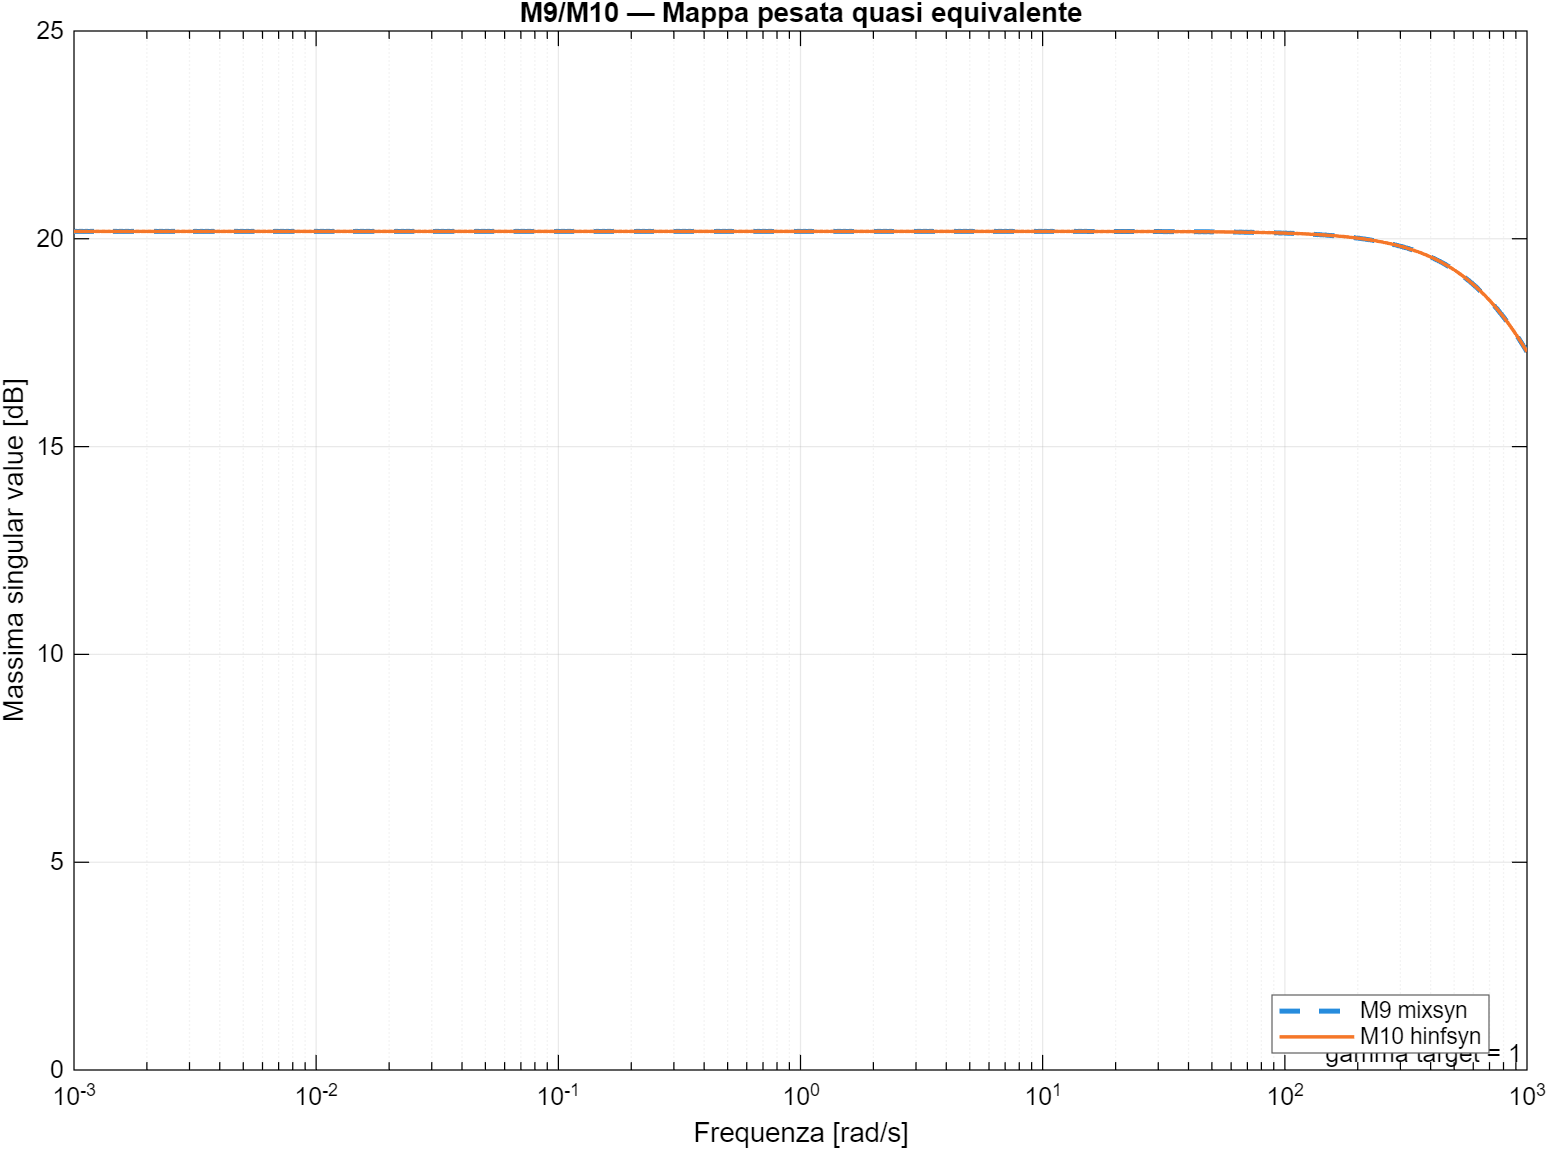
\includegraphics[width=0.88\textwidth]{figures/m10_weighted_comparison_m9.png}
\caption{Baseline originale M9/M10: la sovrapposizione delle mappe verifica l'equivalenza delle interconnessioni, non il soddisfacimento del target uno.}
\label{fig:m10-weighted}
\end{figure}
La Figura~\ref{fig:m10-weighted} conserva il risultato iniziale.
Non vengono sovrascritti gli artifact M9 o M10 e non si introduce
un prefiltro per alterarne retroattivamente le risposte.

\section{Revisione motivata: normalizzazione e terzo canale}
\subsection{Separare cambio di unità e cambio del requisito pesato}
Nel nuovo studio si definiscono
\[
r_N=r/q_s,\quad q_N=q/q_s,\quad u_N=u/u_s,\qquad
G_N=\frac{u_s}{q_s}G,\quad q_s=5\pi/180,\quad u_s=12.
\]
Il controllore fisico è $K=(u_s/q_s)K_N$.
Un puro cambio di coordinate, con tutti i pesi trasformati in modo
equivalente, mantiene la vecchia norma $10.207$; questo viene controllato.
La modifica progettuale è invece adottare
\[
W_{2,N}(s)=\beta_U\frac{s/30+1}{s/180+1}I_2,\qquad
W_{2,\mathrm{fisico}}=\frac{q_s}{u_s}W_{2,N}.
\]
Per $\beta_U=1$ si confrontano il riferimento normalizzato da 5 gradi
e il comando normalizzato su 12 N m. È un rilassamento dichiarato del
peso fisico rispetto alla baseline, non una semplice riscrittura
equivalente. Per $\beta_U=2$ la penalità di comando raddoppia.
La prova diagnostica ID 1 modifica soltanto questa scala e mantiene
$W_1$ e l'assenza di $W_3$: $\gamma$ scende a circa $3.448$,
ma resta maggiore di uno.

\subsection{Perché introdurre \texorpdfstring{$W_3T$}{W3T}}
Un peso su $T$ permette di richiedere attenuazione del rumore di misura
alle alte frequenze e roll-off dell'uscita prima delle dinamiche poco
affidabili. Nel progetto esistono attuatori finiti, un'approssimazione
Padé e rumore encoder, ma non un inviluppo quantitativo del docente
che determini univocamente $W_3$.

La scelta del nuovo studio è pertanto esplicitamente progettuale:
\[
W_3(s)=\frac{s/\omega_T+0.1}{s/(5\omega_T)+1}I_2,\qquad
\omega_T\in\{40,80\}\ {\rm rad/s}.
\]
Il guadagno DC è $0.1$, quello ad alta frequenza è 5.
Lo zero è $0.1\omega_T$, il polo è $5\omega_T$ e il crossover
è $\omega_T\sqrt{0.99/0.96}$, circa $1.0155\omega_T$.
I due valori collocano la transizione presso $\omega_n$ oppure
$2\omega_n$: una richiesta più precoce e una meno restrittiva.
Non sono un'identificazione dello spettro di rumore.

Il peso d'incertezza $W_I$ di M4 descrive invece perturbazioni
moltiplicative all'ingresso degli attuatori. Nel caso MIMO
la complementarità d'ingresso è $T_i=KG(I+KG)^{-1}$ e non coincide
in generale con $T=GK(I+GK)^{-1}$. Perciò usare direttamente
$W_I$ come peso di $T$ non fornirebbe automaticamente il certificato
M4. Il nuovo $W_3$ è un peso di progetto nominale; la $\mu$-analysis
rimane una verifica separata.

\subsection{Campagna deterministica e criteri dichiarati}
Si mantengono $A_s=0.05$, $M_s=2$, $\omega_U=30$,
$\alpha=6$ e tutti i target temporali M5.
La campagna incrocia
\[
\omega_B\in\{8,12,16\},\quad
\beta_U\in\{1,2\},\quad \omega_T\in\{40,80\}.
\]
Le tre bande sono $\omega_n/5$, $0.3\omega_n$, $0.4\omega_n$:
inquadrano una richiesta meno aggressiva, quella originale e una più
aggressiva, senza fingere che la prima garantisca il settling M5.
Sono 12 candidati a tre pesi, più il diagnostico ID 1 senza $W_3$.
Si eseguono inoltre una verifica \texttt{hinfsyn} equivalente sul candidato
illustrativo e una sintesi diagnostica con il solo peso di comando:
15 sintesi in totale, non una ricerca casuale.

Il diagnostico sul solo comando normalizzato restituisce circa
$0.4081$, ma non impone tracking e non è un'alternativa utilizzabile.
Mostra che non è corretto attribuire il mancato $\gamma<1$
alla sola penalizzazione del comando: conta il compromesso con $W_1$,
la stabilizzazione e, quando presente, $W_3$.

Ogni candidato viene valutato su stabilità della matrice plant--controller
completa, norma dello stack, tre norme componenti, due gradini da 5 gradi,
settling, overshoot, errore statico, cross-coupling, picco e RMS di comando.
La selezione illustrativa considera solo candidati a tre pesi stabili
e ordina lessicograficamente: eventuale $\gamma<1$, numero di target M5
violati, massimo rapporto fra metrica temporale e target, picco relativo
di comando, cross-coupling, infine $\gamma$. Non vi è uno score nascosto.
Poiché tutti violano i tre target, il candidato ID 10 viene scelto
per il confronto temporale; non è quello a $\gamma$ minimo e non è
promosso a controllore finale.

\begin{table}[htbp]\centering\small
\begin{tabular}{p{2.1cm}p{3.1cm}p{3.1cm}p{5.1cm}}\toprule
Parametro & Originale & Illustrativo ID 10 & Motivazione \\\midrule
$W_1$: $A_s,M_s$ & $0.05,2$ & invariati & Nessun rilassamento dell'obiettivo statico o del parametro di picco \\
$W_1$: $\omega_B$ & 12 & 16 rad/s & Estremo più aggressivo della terna, scelto dal criterio temporale dichiarato \\
$W_2$: scala & $1/12$ & $(5\pi/180)/12$ & Confronto fra riferimento da 5 gradi e comando da 12 N m, dichiaratamente meno restrittivo \\
$W_2$: zero/polo & $30/180$ & invariati & Stessa penalizzazione relativa dei comandi rapidi \\
$W_3$ & assente & DC 0.1, HF 5, $\omega_T=40$ & Roll-off nominale presso la dinamica attuativa; scelta del progetto \\\bottomrule
\end{tabular}
\caption[Revisione motivata dei pesi]{Modifiche del problema pesato, non dei target temporali M5 o dell'insieme incerto M4.}
\label{tab:hinf-pesi-nuovi}
\end{table}

\subsection{Pianta generalizzata a tre pesi e verifiche indipendenti}
Con i segnali normalizzati, $z_3=W_3q_N$ si aggiunge agli altri
due canali:
\[
P_N=
\begin{bmatrix}
W_1&-W_1G_N\\
0&W_{2,N}\\
0&W_3G_N\\
I&-G_N
\end{bmatrix},\qquad
F_\ell(P_N,K_N)=
\begin{bmatrix}W_1S\\W_{2,\mathrm{fisico}}KS\\W_3T\end{bmatrix}.
\]
La pianta è $8\times4$: sei uscite prestazionali, due misure,
due ingressi esogeni e due comandi. \texttt{connect} usa una sola
istanza di $G_N$. La formula a blocchi e \texttt{augw} sono confronti
indipendenti in frequenza; la lower LFT viene confrontata con lo stack
ricostruito dalla chiusura fisica. \texttt{mixsyn} e
\texttt{hinfsyn(PN,2,2)} restituiscono objective coerenti.
Il numero $\gamma<1$ avrebbe significato solo rispetto a questi pesi
normalizzati, non rispetto a qualsiasi requisito fisico o alla robustezza M4.

\section{Risultati del nuovo studio e figure didattiche}
% Generated by plot_hinf_revision.m.
\begin{table}[htbp]\centering\small
\begin{tabular}{rrrrrrrr}\toprule
ID & $\omega_B$ & $\beta_U$ & $\omega_T$ & $\gamma$ & OS [\%] & picco $u$ & stabili/5 \\\midrule
0 & 12 & 11.459 & 0 & 10.207 & 261.62 & 5.1599 & 5 \\
1 & 12 & 1 & 0 & 3.4477 & 155.9 & 14.19 & 2 \\
2 & 8 & 1 & 40 & 2.8302 & 149.13 & 11.859 & 3 \\
3 & 8 & 1 & 80 & 2.8056 & 152.82 & 11.956 & 3 \\
4 & 8 & 2 & 40 & 3.6641 & 180.56 & 8.7844 & 4 \\
5 & 8 & 2 & 80 & 3.6476 & 186.15 & 8.829 & 4 \\
6 & 12 & 1 & 40 & 3.4886 & 145.41 & 13.952 & 3 \\
7 & 12 & 1 & 80 & 3.4624 & 151.62 & 14.069 & 2 \\
8 & 12 & 2 & 40 & 4.4659 & 175.43 & 10.222 & 3 \\
9 & 12 & 2 & 80 & 4.4561 & 180.17 & 10.297 & 3 \\
10 & 16 & 1 & 40 & 4.073 & 144.44 & 15.686 & 2 \\
11 & 16 & 1 & 80 & 4.0464 & 153.38 & 15.818 & 2 \\
12 & 16 & 2 & 40 & 5.1858 & 169.39 & 11.438 & 3 \\
13 & 16 & 2 & 80 & 5.1687 & 173.44 & 11.51 & 3 \\
\bottomrule\end{tabular}
\caption{Campagna deterministica. ID 0 è la baseline ricaricata; ID 1 isola la nuova scala di comando senza $W_3$. Le frequenze sono in rad/s, il comando in N m. Tutti sono nominalmente stabili; nessuno supera tutti i target M5. I cinque campioni M4 non certificano robustezza.}
\label{tab:hinf-campagna}\end{table}
\begin{table}[htbp]\centering\small
\begin{tabular}{lrr}\toprule
Metrica & M10 originale & candidato illustrativo \\\midrule
$\gamma$ & 10.207 & 4.073 \\
$\|W_1S\|_\infty$ & 10.128 & 4.0702 \\
$\|W_2KS\|_\infty$ & 10.185 & 4.0339 \\
$\|W_3T\|_\infty$ & 0 & 2.5921 \\
$T_s$ [s] & 1.566 & 1.162 \\
Overshoot [\%] & 261.62 & 144.44 \\
Errore statico relativo & 0.49068 & 0.20143 \\
Cross-coupling & 0.2596 & 0.19912 \\
Picco comando [N m] & 5.1599 & 15.686 \\
RMS comando [N m] & 1.0517 & 1.1913 \\
Ordine & 18 & 20 \\
\bottomrule\end{tabular}
\caption{Metriche peggiori fra due gradini nominali separati da 5 gradi, 12 s, senza disturbi o rumore. I valori $\gamma$ riguardano problemi pesati diversi: non sono direttamente una graduatoria di robustezza.}
\label{tab:hinf-nuovo-confronto}\end{table}

Il miglior $\gamma$ della campagna è circa $2.806$ (ID 3);
nessun candidato raggiunge uno. Il candidato illustrativo ID 10 ha
$\gamma\simeq4.073$, $T_s=1.162$ s, overshoot $144.44\%$ e
picco di comando $15.686$ N m. Il miglioramento rispetto alla baseline
non rende questi valori accettabili. Le norme di problemi pesati
diversi non costituiscono da sole una misura comparabile di qualità.

La Figura~\ref{fig:hinf-pesi-rivisti} mostra le modifiche ai pesi.
La Figura~\ref{fig:hinf-inviluppi} risponde invece alla domanda
se le due direzioni singolari di $S$ e $T$ rispettino gli inviluppi
scelti. Il confronto scalare è corretto perché ogni peso è un filtro
scalare replicato sui due canali, non una matrice arbitraria.
\begin{figure}[htbp]\centering
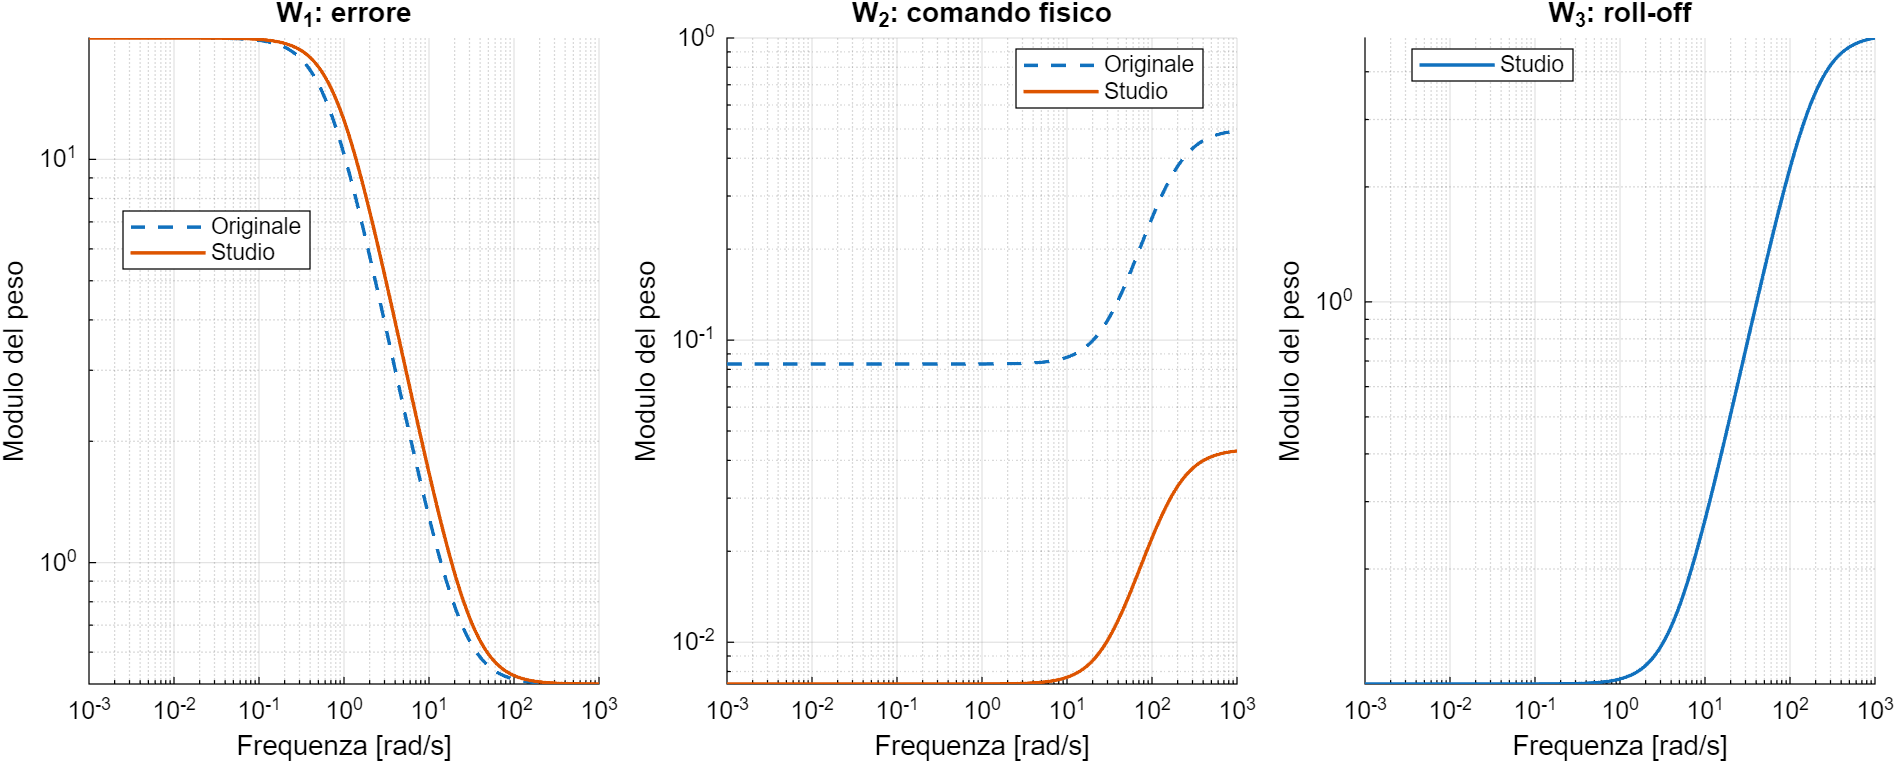
\includegraphics[width=0.98\textwidth]{figures/hinf_revision_weights.png}
\caption{Pesi fisici originali e del candidato ID 10. Il vecchio $W_3$ è assente, non un filtro non nullo nascosto sotto il grafico.}
\label{fig:hinf-pesi-rivisti}
\end{figure}
\begin{figure}[htbp]\centering
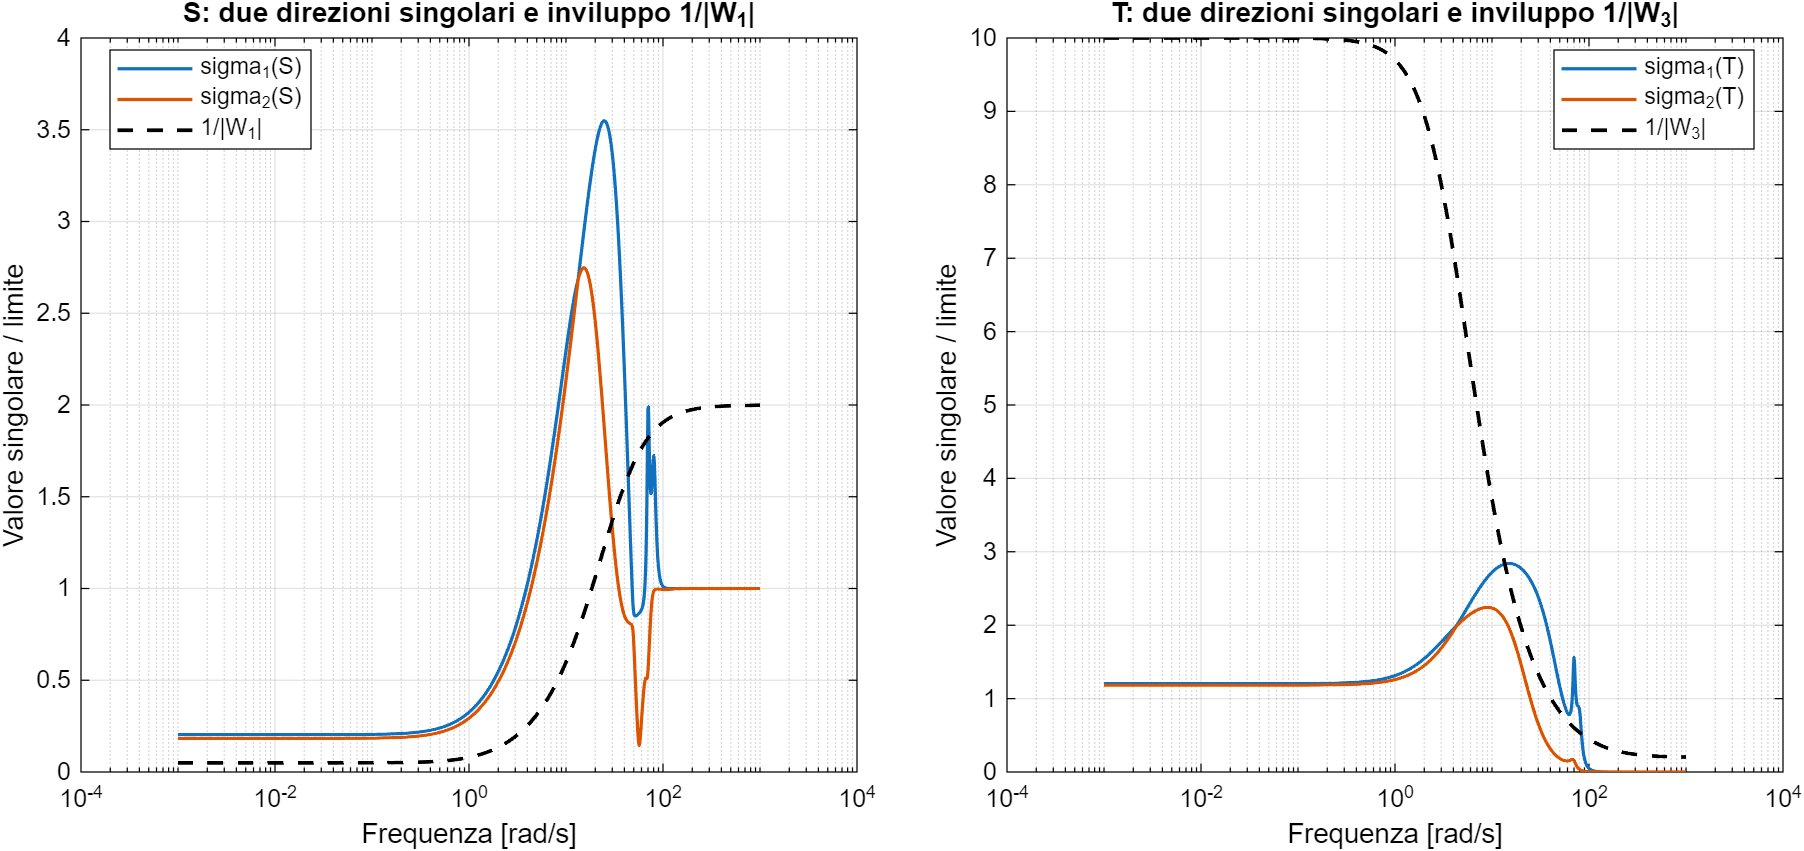
\includegraphics[width=0.96\textwidth]{figures/hinf_revision_sensitivity_envelopes.png}
\caption{Valori singolari di $S$ e $T$ confrontati rispettivamente con $1/|W_1|$ e $1/|W_3|$. Gli inviluppi sono obiettivi del nuovo problema, non certificati di robustezza.}
\label{fig:hinf-inviluppi}
\end{figure}

La Figura~\ref{fig:hinf-canali-rivisti} espone direttamente i tre
contributi e il livello uno. La norma dello stack non è semplicemente
il massimo delle tre norme: i canali si sommano quadraticamente
nella matrice prestazionale prima della massimizzazione.
\begin{figure}[htbp]\centering
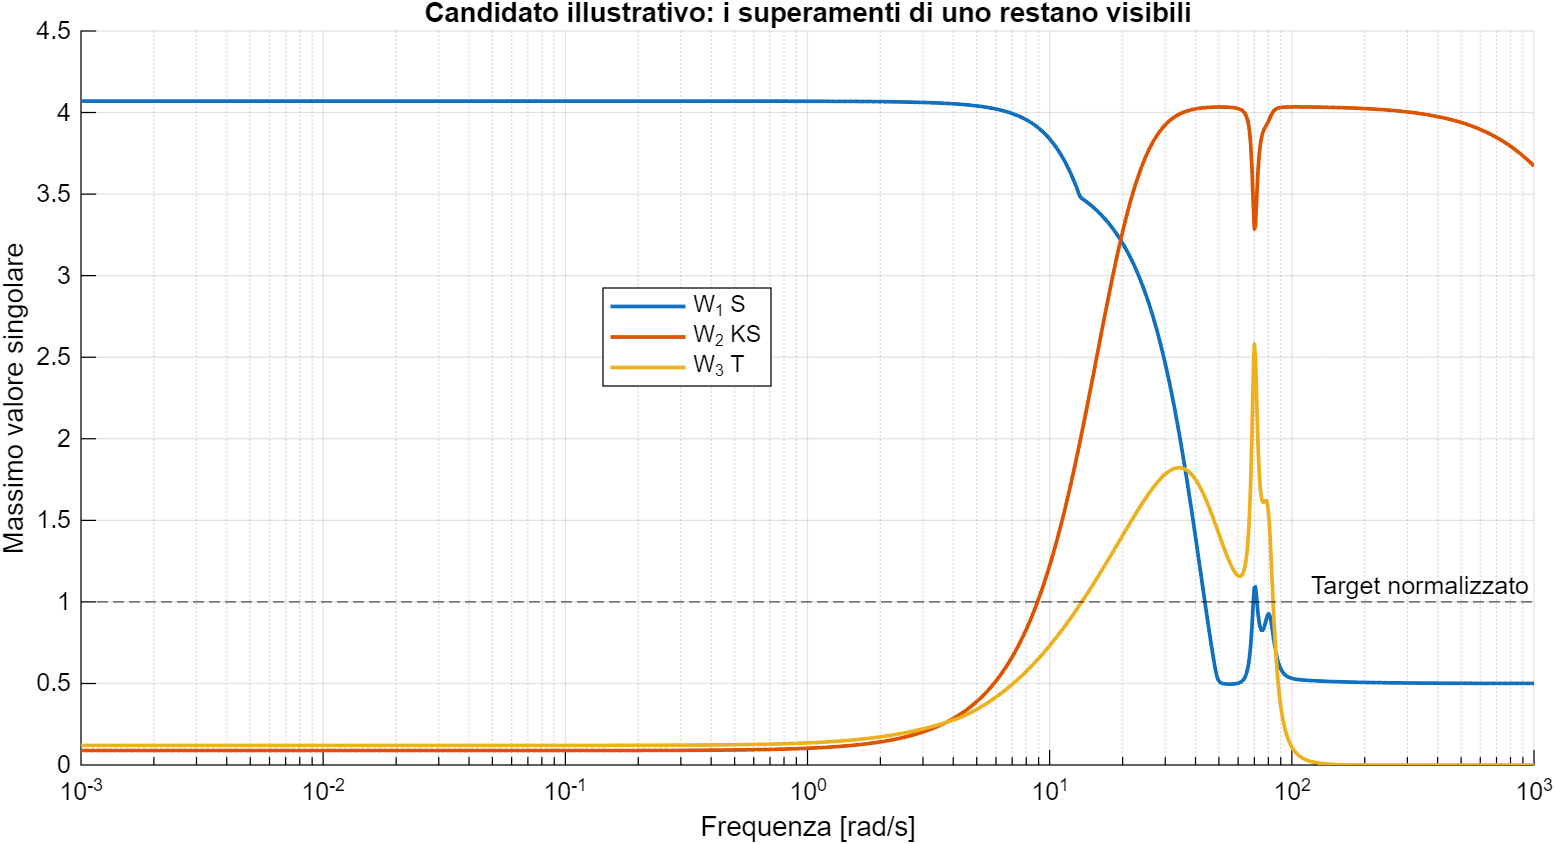
\includegraphics[width=0.86\textwidth]{figures/hinf_revision_weighted_channels.png}
\caption{Massimi valori singolari di $W_1S$, $W_2KS$, $W_3T$ per ID 10. Tutti i superamenti del target sono conservati.}
\label{fig:hinf-canali-rivisti}
\end{figure}
La Figura~\ref{fig:hinf-tempo-rivisto} mostra due esperimenti separati
con stesso orizzonte di 12 s, stato nullo, nessun disturbo o rumore.
Le colonne distinguono il giunto di riferimento, le righe posizioni
e comandi. L'overshoot molto elevato e l'offset finale spiegano
perché il risultato non venga selezionato come controllore del progetto.
\begin{figure}[htbp]\centering
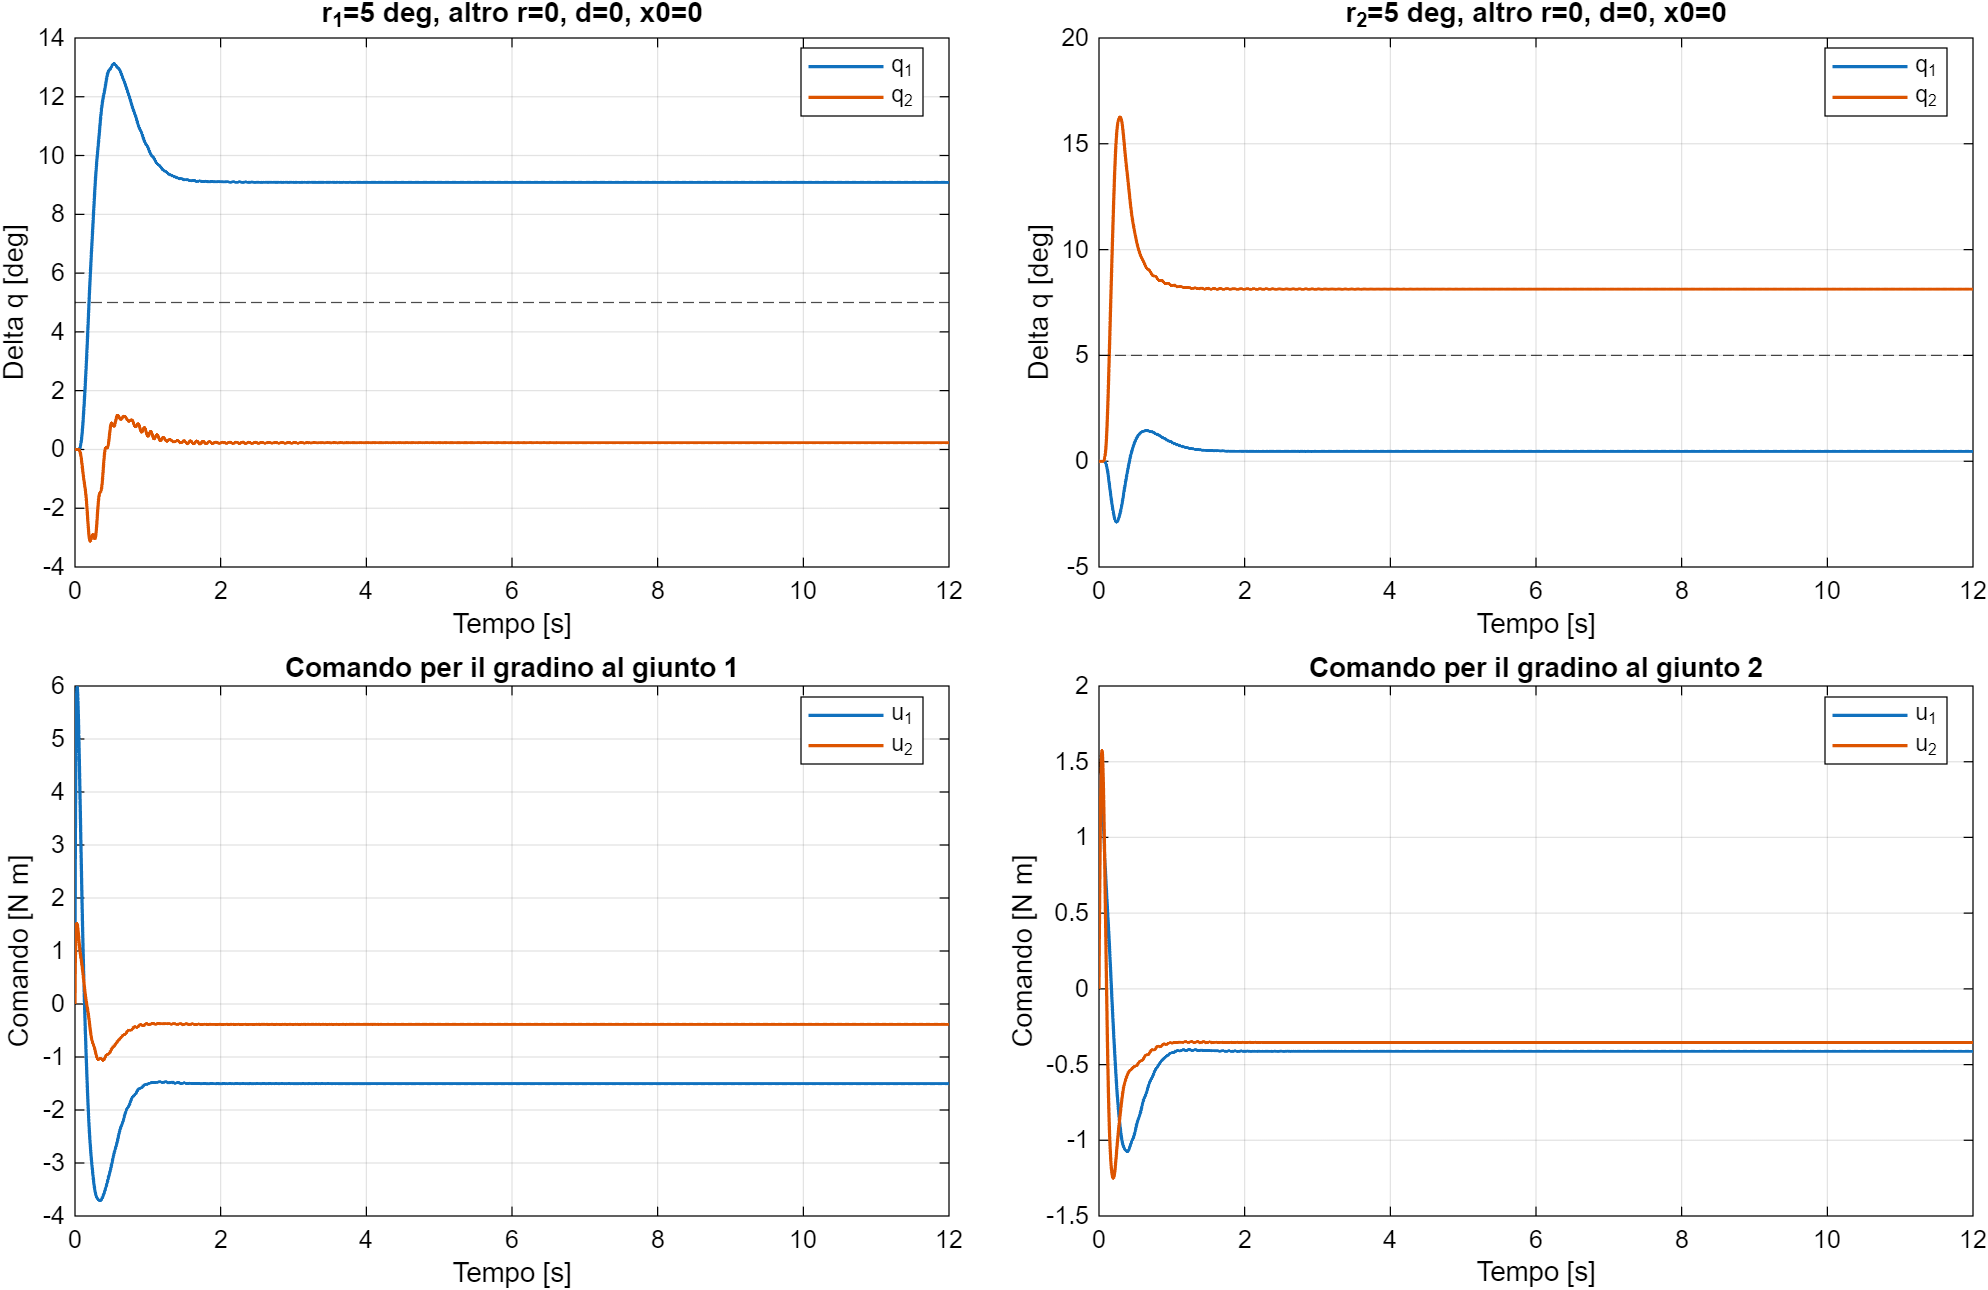
\includegraphics[width=0.95\textwidth]{figures/hinf_revision_tracking_control.png}
\caption{Tracking e comando di ID 10 per gradini da 5 gradi. La linea tratteggiata indica il riferimento del giunto eccitato; l'altro riferimento è nullo. Nessun prefiltro o saturazione è aggiunto.}
\label{fig:hinf-tempo-rivisto}
\end{figure}

Cinque campioni M4 comuni, seed 20260910, completano il controllo
esplorativo: ID 10 è stabile soltanto in 2/5 casi, mentre la baseline
M10 lo è in 5/5. Non sono i 40 campioni ufficiali M16 e le frazioni
non sono probabilità o certificati. Non emerge pertanto una ragione
per sostituire la baseline robusta con il nuovo candidato.

\section{M11: full-order, strutture implementabili e analisi successive}
Il controllore full-order viene ottenuto senza imporre a priori
una struttura a basso ordine. Il nuovo problema a tre pesi produce
ordine 20, contro 18 della baseline: si aggiungono due stati di peso.
Un ordine maggiore aumenta la libertà dinamica, ma non garantisce
automaticamente un miglior risultato utile o una maggiore robustezza.

M11 rimane lo studio strutturato del problema originale, non viene
rinominato come risultato dei nuovi pesi. Comprende guadagno statico
MIMO, due PI decentralizzati, due PID filtrati e tre strutture MIMO
di ordine 2, 4, 6, con cinque partenze per famiglia.
A0/A1 non producono objective finiti, A2 non produce chiusure stabili;
A3/A4/A5 danno cinque soluzioni stabili ciascuna. I migliori objective
sono circa $16.6419$, $11.6555$ e \AFiveGamma.
La maggiore flessibilità riduce il divario dal full-order, a costo
di più stati e parametri. Le ottimizzazioni strutturate non sono
necessariamente globali: le partenze multiple documentano questo limite.

\begin{figure}[htbp]\centering
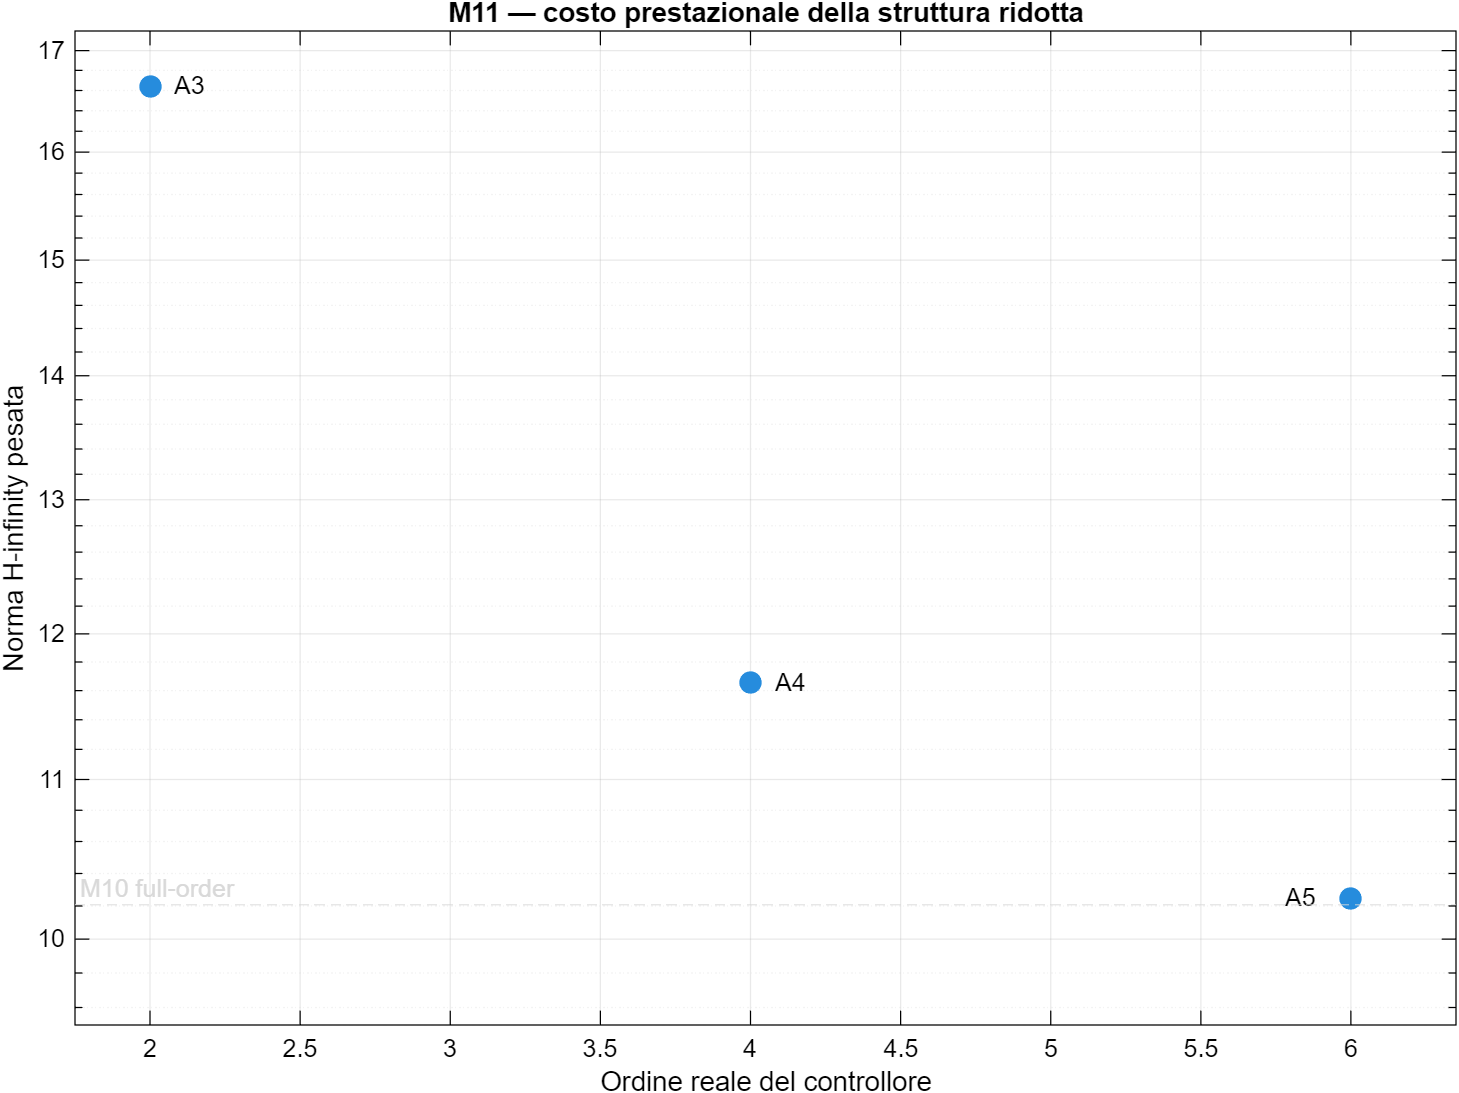
\includegraphics[width=0.80\textwidth]{figures/m11_gamma_vs_order.png}
\caption{Frontiera ordine--objective della baseline M11. Non sono risultati della nuova campagna a tre pesi.}
\label{fig:m11-order}
\end{figure}
La Figura~\ref{fig:m11-order} e la tabella seguente mantengono il confronto
storico. A5, ordine 6, è il candidato strutturato M12; non coincide
con $K_\infty$ M10, ordine 18.
% Tabella generata da build_m18_report_tables.m.
\begin{table}[H]
\centering
\begin{tabular}{lllll}
\toprule
Controllore & Ordine & $\gamma$/objective & NS & NP \\
\midrule
M9 mixsyn & 18 & 5.6772 & PASS & FAIL \\
M10 hinfsyn & 18 & 5.6772 & PASS & FAIL \\
M11 A3 & 2 & 8.1671 & PASS & FAIL \\
M11 A4 & 4 & 5.9672 & PASS & FAIL \\
M11 A5 & 6 & 5.7086 & PASS & FAIL \\
\bottomrule
\end{tabular}
\caption{Sintesi nominali H-infinity. Un valore $\gamma>1$ non costituisce PASS prestazionale.}
\label{tab:hinf}
\end{table}


La nuova campagna non modifica gli artifact o la pianta generalizzata
delle fasi M9--M16 originali. Poiché nessun nuovo candidato supera
l'insieme dei target e il comportamento incerto peggiora, non viene
adottato un nuovo peso nella catena di produzione. Non occorre
rieseguire M11, D--K, M14 o M16 per attribuire loro risultati nuovi
che non esistono. Se in futuro si promuovesse un nuovo controllore,
quelle verifiche dovrebbero essere ripetute sul problema corrispondente.
La sintesi nominale $H_\infty$ non sostituisce la successiva
$\mu$-analysis; neppure l'aggiunta di $W_3$ trasferisce automaticamente
al candidato il certificato di $K_\mu$.

\chapter{\texorpdfstring{Robustezza alle incertezze: analisi e sintesi con $\mu$}{Robustezza alle incertezze: analisi e sintesi con mu}}
\label{cap:mu}
\section{Dalle prove nominali alle incertezze fisiche}
Le prove del capitolo precedente descrivono il comportamento del
controllore sul modello nominale. A questo punto vogliamo capire
che cosa succede quando i parametri reali del manipolatore differiscono
 dai valori nominali. Una rigidezza diversa sposta le risonanze SEA;
un'inerzia motore diversa modifica la dinamica interna; una dinamica
attuativa non modellata può alterare modulo e fase del feedback.

La domanda non è più se un singolo modello risponde bene, ma se
il sistema rimane stabile e rispetta la prestazione pesata per
\emph{tutta} la famiglia ammessa. Confrontiamo il controllore
$H_\infty$ 2-DoF e $K_\mu$ mantenendo gli stessi $W_e,W_u,M_o$,
lo stesso disturbo lato link e la stessa mappa $[r;d]\mapsto[z_e;z_u]$.
Le incertezze sono quelle del Capitolo 5, dichiarate prima della sintesi.

\subsection{I tre parametri meccanici selezionati}
Sono incerti $k_1,k_2$ e $J_{m1}$, indipendenti e reali.
Le rigidezze possono variare per materiali e assemblaggio; l'inerzia
riflessa del primo motore dipende anche dalla modellazione
 dell'azionamento. Il 10\% è un'ipotesi ingegneristica del progetto,
non una tolleranza misurata né un intervallo statistico.

\begin{table}[htbp]\centering\small
\begin{tabular}{lrrl}\toprule
Parametro & Nominale & Intervallo & Oggetto MATLAB\\\midrule
$k_1$ [N m/rad] & 50 & $[45,55]$ & \texttt{ureal('k1',50,\ldots)}\\
$k_2$ [N m/rad] & 40 & $[36,44]$ & \texttt{ureal('k2',40,\ldots)}\\
$J_{m1}$ [kg m$^2$] & 0.01 & $[0.009,0.011]$ & \texttt{ureal('Jm1',0.01,\ldots)}\\\bottomrule
\end{tabular}
\caption{I tre scalari reali usano \texttt{'Percentage',10},
come definito nella funzione centrale dei parametri incerti.}
\end{table}
Masse, geometrie, $J_{m2}$, attriti e gravità restano nominali.
È una scelta per contenere il numero di parametri incerti,
non una dichiarazione che siano fisicamente esatti.

\subsection{La dinamica degli attuatori}
Per costruire la famiglia attuativa si variano frequenza naturale,
smorzamento e ritardo. Le prime due influenzano rapidità e risonanza;
il ritardo include dispersioni di latenza e jitter.

\begin{table}[htbp]\centering
\begin{tabular}{lrrr}\toprule
Grandezza & Nominale & Variazione & Intervallo\\\midrule
$\omega_n$ [rad/s] & 40 & $\pm10\%$ & $[36,44]$\\
$\zeta$ & 0.8 & $\pm10\%$ & $[0.72,0.88]$\\
Ritardo [ms] & 15 & $\pm20\%$ & $[12,18]$\\\bottomrule
\end{tabular}
\caption{Intervalli usati per costruire l'inviluppo degli errori
attuativi; non sono tre ulteriori blocchi \texttt{ureal} nella pianta finale.}
\end{table}
La famiglia contiene 120 attuatori: nominale, sei variazioni singole,
otto vertici e 105 campioni riproducibili. L'errore relativo rispetto
all'attuatore nominale è raccolto nell'inviluppo
\[
 W_I(s)=\frac{2.929983729s+3.748469010}{s+206.973575453}.
\]
Il fit usa margine 1.08 e il massimo rapporto campionato
 fra errore relativo e inviluppo è 0.92593. Questa verifica
copre i campioni costruiti, non ogni possibile attuatore fisico.
La rappresentazione finale per ciascun canale è
\[
 G_{ai}^{\Delta}=G_{a0}(1+W_I\Delta_{ai}),\qquad
 \|\Delta_{ai}\|_\infty\le1,\quad i=1,2.
\]
$\Delta_{ai}$ è una dinamica scalare stabile ignota, rappresentata
con \texttt{ultidyn}. I due canali sono indipendenti.
Nell'analisi robusta si considera tutto questo insieme matematico,
più ampio della sola lista di attuatori usata per il fit.

\section{Raccogliere le incertezze in \texorpdfstring{$\Delta$}{Delta}}
Per passare dalle grandezze fisiche a una rappresentazione comune,
esprimiamo i parametri come scostamenti normalizzati. Per esempio
\[
 k_1=50(1+0.1\delta_{k1}),\qquad \delta_{k1}\in[-1,1].
\]
$\delta_{k1}=0$ è il nominale; $\delta_{k1}=1$ dà 55 N m/rad.
La stessa idea vale per $k_2$ e $J_{m1}$. La normalizzazione
non cambia gli intervalli: rende la soglia uno comune ai blocchi.
Le dipendenze fisiche, incluso l'inverso di $J_{m1}$, sono
conservate nel modello; non si aggiunge un errore arbitrario ad $A$.

MATLAB estrae la struttura
\begin{equation}\label{eq:deltafive}
 \Delta=\operatorname{diag}(\Delta_{a1},\Delta_{a2},
 \delta_J,\delta_{k1},\delta_{k2})\in\mathbb C^{5\times5}.
\end{equation}
I primi due blocchi sono dinamici scalari complessi, gli ultimi tre
scalari reali. Il campo \texttt{Occurrences} vale uno per ciascuno
 dei cinque blocchi nella rappresentazione salvata. Non si conta
il numero di blocchi dal numero di apparizioni del simbolo nelle
 equazioni. Le due dinamiche non sono fuse in un blocco pieno
$2\times2$, che ammetterebbe accoppiamenti diversi da quelli scelti.

\section{Separare la parte nota: lo schema \texorpdfstring{$N$--$\Delta$}{N--Delta}}
Fissiamo prima il controllore. Possiamo poi vedere il sistema
chiuso come due parti collegate: $N$ contiene ciò che conosciamo,
compresi il controllore e i pesi; $\Delta$ contiene gli scostamenti
ammessi. $N$ manda il segnale $v_\Delta$ alla parte incerta e ne
riceve $w_\Delta=\Delta v_\Delta$. Questa è la rappresentazione
$N$--$\Delta$ mostrata in Figura~\ref{fig:ndelta}.

\begin{figure}[htbp]\centering
\begin{tikzpicture}[>=stealth,thick,
 b/.style={draw,rounded corners,align=center,text width=4.6cm},
 every node/.style={font=\small}]
\node[b,minimum height=1.6cm] (n) at (0,0)
 {$N$: parte nota\\pianta, pesi e controllore fissato};
\node[b,minimum height=1.2cm] (d) at (0,2.6)
 {$\Delta$: parte incerta\\due dinamiche + tre parametri reali};
\draw[->] (n.east |- 0,.55) -- (3.4,.55) -- (3.4,2.6)
 -- node[above] {$v_\Delta$} (d.east);
\draw[->] (d.west) -- (-3.4,2.6) -- (-3.4,.55)
 -- node[above] {$w_\Delta$} (n.west |- 0,.55);
\draw[->] (-4.7,-.55) node[left] {$w=[r;d]$} -- (n.west |- 0,-.55);
\draw[->] (n.east |- 0,-.55) -- (4.7,-.55) node[right] {$z=[z_e;z_u]$};
\node at (0,-1.1) {$w_\Delta=\Delta v_\Delta$};
\end{tikzpicture}

\caption{A controllore fissato, $N$ raccoglie la parte nota e
$\Delta$ i cinque blocchi incerti. $w=[r;d]$ e $z=[z_e;z_u]$
conservano il significato del Capitolo 8.}\label{fig:ndelta}
\end{figure}
Solo dopo aver distinto le due parti scriviamo le loro connessioni:
\[
 \begin{bmatrix}v_\Delta\\z\end{bmatrix}
 =\begin{bmatrix}N_{11}&N_{12}\\N_{21}&N_{22}\end{bmatrix}
 \begin{bmatrix}w_\Delta\\w\end{bmatrix},\qquad
 w_\Delta=\Delta v_\Delta.
\]
$N_{11}$ è il ritorno fra le porte dell'incertezza;
$N_{22}$ è la mappa nominale esterna quando $\Delta=0$.
Nel nostro caso $N$ è $9\times9$, con cinque canali interni
 e quattro ingressi esterni/uscite pesate. Quindi $N_{11}$
è $5\times5$ e $N_{22}$ è $4\times4$.

La LFT è il modo compatto di indicare questa connessione.
La chiusura di $K$ su $P_\Delta$ è una LFT inferiore;
la separazione di $\Delta$ da $N$ è una LFT superiore.
Nel codice la matrice chiamata $N$ nel testo è \texttt{M}:
\begin{lstlisting}
CL=lft(P,K);
[M,Delta,BlkStruct,NormUnc]=lftdata(CL);
CLcheck=lft(Delta,M);
\end{lstlisting}
La terza riga ricompone il modello nella convenzione MATLAB.
Non va invertito l'ordine degli argomenti mantenendo la stessa
partizione. La ricostruzione nominale è stata verificata; le
formule complete sono nell'Appendice~\ref{app:matlab}.

\section{Che cosa misura \texorpdfstring{$\mu$}{mu}}
$\mu$ aiuta a capire quanto la struttura d'incertezza ammessa è
vicina a causare una condizione critica. Si cerca la più piccola
perturbazione, con gli stessi tipi di blocchi, capace di rendere
singolare il ritorno interno $I-N_{11}\Delta$. $\mu$ è l'inverso
 della sua grandezza.

Se il picco di $\mu$ è minore di uno, la condizione critica
richiede un'incertezza più grande di quella normalizzata ammessa,
con le usuali ipotesi di stabilità nominale e buona posizione
 dell'interconnessione. Se supera uno, la robusta stabilità
può venire meno già entro il dominio dichiarato.
Non è una probabilità di guasto: tiene conto della struttura,
non di una distribuzione statistica delle incertezze.

Il calcolo esatto è difficile, quindi si usano due limiti
$\underline\mu\le\mu\le\overline\mu$.
La maggiorazione serve a escludere una criticità nel dominio;
la minorazione deriva dalla ricerca di perturbazioni critiche.
Se i limiti non permettono una decisione rispetto alla soglia
uno, il risultato rimane inconclusivo. Scaling D, e anche G
per i blocchi reali, servono a calcolare queste maggiorazioni.
Il loro dettaglio numerico non modifica il significato fisico
 dei cinque blocchi.

\section{Prestazione nominale, stabilità e prestazione robuste}
\subsection{Prima il caso nominale: NS e NP}
NS richiede stabilità interna per $\Delta=0$.
NP aggiunge $\|T_{zw,0}\|_\infty<1$.
La stabilità è controllata prima della norma, sulla realizzazione
completa. NP non equivale a rispettare tutti i target temporali:
il capitolo precedente ha mostrato un $H_\infty$ con NP positiva
 e assestamento oltre 0.8 s.

\subsection{Stabilità robusta: RS}
RS chiede stabilità per tutte le incertezze ammesse.
Si studia il ritorno $N_{11}$ con la struttura fisica $\Delta$.
Il margine $m_{RS}$ dice di quanto si possono amplificare insieme
 gli scostamenti normalizzati prima della condizione critica.
Per esempio, un margine maggiore di uno copre il dominio scelto;
un margine minore di uno indica che esso è troppo ampio per il
controllore considerato.

Il codice corrente usa \texttt{robstab}, che restituisce limiti
 inferiore e superiore del margine. Se il limite inferiore supera
uno, RS è soddisfatta nel modello; se quello superiore è sotto
uno, RS è esclusa. Se l'intervallo attraversa uno, non si accredita
la proprietà. I margini non sono valori di $\mu$.

\subsection{Prestazione robusta: RP}
RP richiede stabilità e $\|T_{zw}(\Delta)\|_\infty<1$ per tutta
la famiglia. Un sistema può quindi essere robustamente stabile
 ma non rispettare le prestazioni pesate.
Per interpretare RP si può aggiungere un blocco fittizio di
prestazione che richiude $z$ su $w$. Nel nostro problema è un
blocco complesso pieno $\Delta_p$ di dimensione $4\times4$:
non è un nuovo parametro fisico del robot.

\begin{figure}[htbp]\centering
\resizebox{.8\textwidth}{!}{\providecommand{\SeaDeltaLabel}{cinque blocchi fisici}
\begin{tikzpicture}[>=stealth,thick,b/.style={draw,align=center,minimum height=1cm,minimum width=3.1cm}]
\node[b] (n) at (0,0) {$N$\\$[w_\Delta;w]\mapsto[v_\Delta;z]$};
\node[b] (d) at (0,2) {$\Delta$: \SeaDeltaLabel};
\node[b] (p) at (0,-2) {$\Delta_p$: pieno $4\times4$};
\draw[->] (n.east |- 0,.3)--(3,.3)--(3,2)--(d.east);
\draw[->] (d.west)--(-3,2)--(-3,.3)--(n.west |- 0,.3);
\draw[->] (n.east |- 0,-.3)--(3,-.3)--(3,-2)--node[below]{$z$}(p.east);
\draw[->] (p.west)--node[below]{$w$}(-3,-2)--(-3,-.3)--(n.west |- 0,-.3);
\end{tikzpicture}
}
\caption{Interpretazione di RP con il blocco fittizio $\Delta_p$.
Le incertezze fisiche conservano la loro struttura.}
\end{figure}
Nel percorso finale si usa \texttt{robgain(CL,1)}: scala le
incertezze fisiche lasciando fissata la soglia prestazionale uno.
Questo margine non è semplicemente l'inverso della norma nominale.
Le chiamate effettive in \path{run_hinf_final_robust.m} sono
\begin{lstlisting}
[a.RS,a.rsWorst,a.rsInfo]=robstab(a.CL);
[a.RP,a.rpWorst,a.rpInfo]=robgain(a.CL,1);
\end{lstlisting}
I nomi \texttt{robuststab} e \texttt{robustperf} non sono usati
nelle chiamate del repository: il progetto impiega \texttt{robstab}
e \texttt{robgain}. Esiste inoltre un calcolo diretto di
\texttt{mussv} su griglia nelle analisi precedenti. L'appendice
lo mostra come esempio della procedura storica, senza trasferirne
i numeri ai controllori finali.

\subsection{Esito del controllore nominale}
Il controllore $H_\infty$ di ordine \FinalOrder\ supera NS e NP,
ma il margine RS è
\[
 m_{RS}\in[\FinalHRSLowerBound,\FinalHRSUpperBound],
 \qquad\omega_{\rm crit}\simeq70.32\ \mathrm{rad/s}.
\]
Entrambi gli estremi sono molto minori di uno. La frequenza è
vicina ai modi elastici: suggerisce una compensazione nominale
fragile in quella zona, senza identificare da sola un parametro
responsabile. L'intervallo RP restituito è invece invertito,
circa $[0.0172543,0.0171945]$, anche dopo la ricerca rinforzata
\texttt{MussvOptions='m9'}. Non ne scambiamo gli estremi:
la stima numerica del margine RP è non validata. RP è comunque
esclusa dal fallimento RS, che è una sua condizione necessaria.

\section{Progettare per le incertezze: \texorpdfstring{$\mu$-synthesis}{mu-synthesis}}
Finora abbiamo analizzato un controllore progettato sul nominale.
La $\mu$-synthesis considera invece le incertezze durante la
sintesi. Nel progetto si usa \texttt{musyn}, con iterazione D--K:
\begin{enumerate}
\item si ottiene un controllore per il problema scalato iniziale;
\item con il controllore fissato si valuta dove l'incertezza è più critica;
\item si aggiornano gli scaling che descrivono il peso delle direzioni critiche;
\item si approssimano gli scaling con trasferimenti razionali;
\item si risintetizza un controllore $H_\infty$ per la pianta scalata;
\item si ripete fino al criterio di arresto o al numero massimo di iterazioni.
\end{enumerate}
Con blocchi reali e dinamici si usano scaling D/G; D--K è il
nome usuale del procedimento. L'alternanza non dimostra un
ottimo globale. Le dinamiche del fit possono aumentare
l'ordine del controllore.

\begin{figure}[htbp]\centering
\resizebox{.94\textwidth}{!}{\begin{tikzpicture}[>=stealth,thick,b/.style={draw,rounded corners,align=center,text width=2.65cm,minimum height=1.3cm}]
\node[b] (k) at (0,0) {Sintesi $H_\infty$\\scaling fissati};
\node[b] (m) at (4,0) {Analisi $\mu$\\$K$ fissato};
\node[b] (f) at (8,0) {Fit razionale\\scaling D/G};
\draw[->] (k)--node[above]{$K_i$}(m);\draw[->] (m)--(f);
\draw[->] (f.south)--(8,-1.5)--node[below]{pianta scalata per l'iterazione successiva}(0,-1.5)--(k.south);
\draw[->] (m.north)--(4,2)node[above,align=center]{Controllore finale fissato\\Post-analisi NS/NP/RS/RP};
\end{tikzpicture}
}
\caption{Iterazione di sintesi. Alla fine il controllore viene
fissato e analizzato sulla pianta incerta originale.}
\end{figure}
La chiamata reale è
\begin{lstlisting}
[K,objective,info]=musyn(P,4,2,opts);
\end{lstlisting}
$P$ è qui la pianta generalizzata incerta 2-DoF; rimangono quattro
segnali $[r;q]$ per il controllore e due comandi.
È stata eseguita una campagna di cinque iterazioni, con
\texttt{MixedMU='on'}, scaling D/G e griglia di 1201 frequenze
fra $10^{-3}$ e $10^4$ rad/s. Opzioni e seed sono salvati
insieme al risultato e riassunti nell'Appendice~\ref{app:matlab}.

\begin{figure}[htbp]\centering
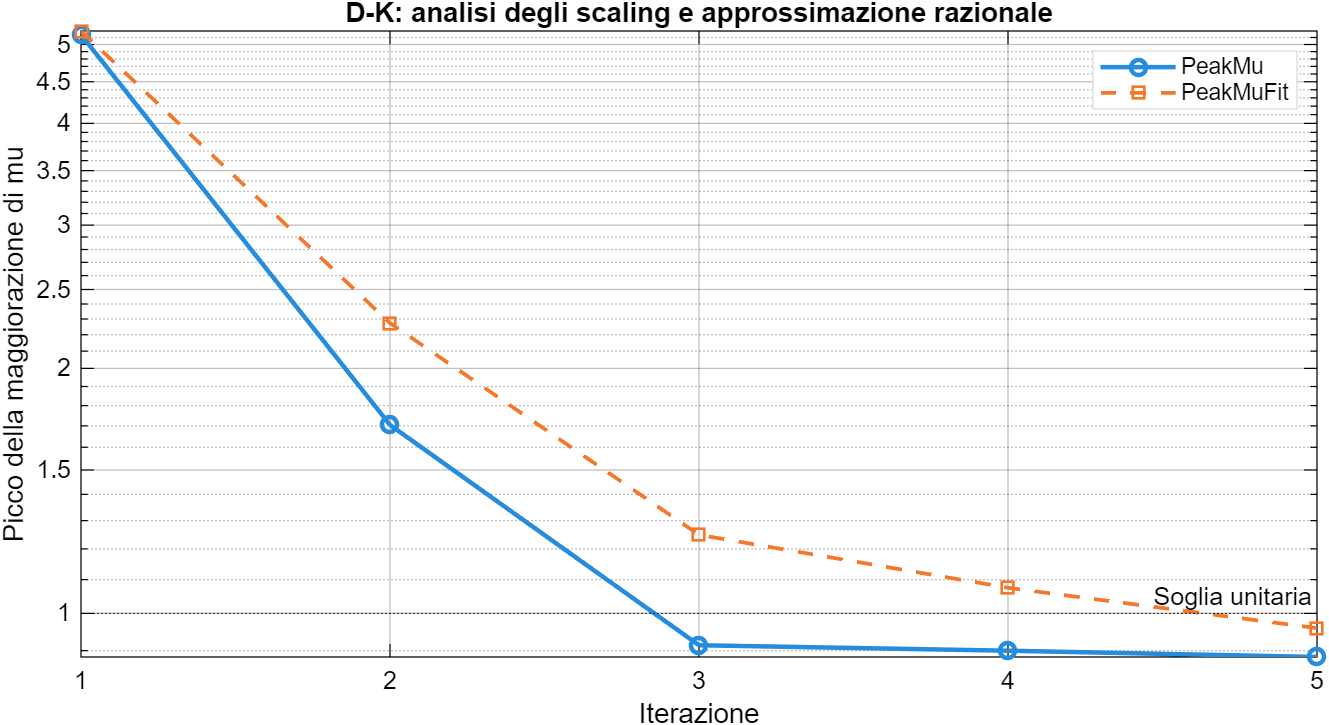
\includegraphics[width=.85\textwidth]{figures/mu/dk_history.png}
\caption{Picchi salvati di $\mu$ e delle rispettive approssimazioni
 dopo il fit. Non sono risultati Monte Carlo.}\label{fig:dkhistory}
\end{figure}
Il picco scende da circa 5.1412 a \FinalMuObjective;
il controllore ottenuto ha ordine \FinalMuOrder.
Il valore finale della sintesi, il picco dopo fit e la norma
nominale sulla pianta originale sono quantità diverse.
Non è stata eseguita una riduzione d'ordine.

\section{Post-analisi e confronto finale di robustezza}
Il controllore salvato viene ricollegato alla stessa pianta
incerta. Si controllano identità del nominale, stabilità interna,
norma e struttura dei blocchi; si ripetono le analisi RS e RP.
I margini non si deducono dal solo obiettivo della sintesi.

\begin{table}[htbp]\centering\small
\begin{tabular}{lcc}\toprule
Quantità & $H_\infty$ 2-DoF & $K_\mu$ 2-DoF\\\midrule
Ordine & \FinalOrder & \FinalMuOrder\\
NS & soddisfatta & soddisfatta\\
Norma nominale & \FinalGamma & \FinalMuGamma\\
NP & soddisfatta & soddisfatta\\
Margine RS & $[\FinalHRSLowerBound,\FinalHRSUpperBound]$ & $[\FinalMuRSLowerBound,\FinalMuRSUpperBound]$\\
Esito RS & non soddisfatta & soddisfatta\\
Margine RP & intervallo non valido & $[\FinalMuRPLowerBound,\FinalMuRPUpperBound]$\\
Esito RP & esclusa da RS & soddisfatta\\
$\omega_{RS}$ [rad/s] & 70.32 & 61.96\\
$\omega_{RP}$ [rad/s] & non accreditata & 9.85\\\bottomrule
\end{tabular}
\caption{Confronto sullo stesso modello incerto e sugli stessi pesi.
Gli intervalli sono limiti del margine.}
\end{table}
\begin{figure}[htbp]\centering
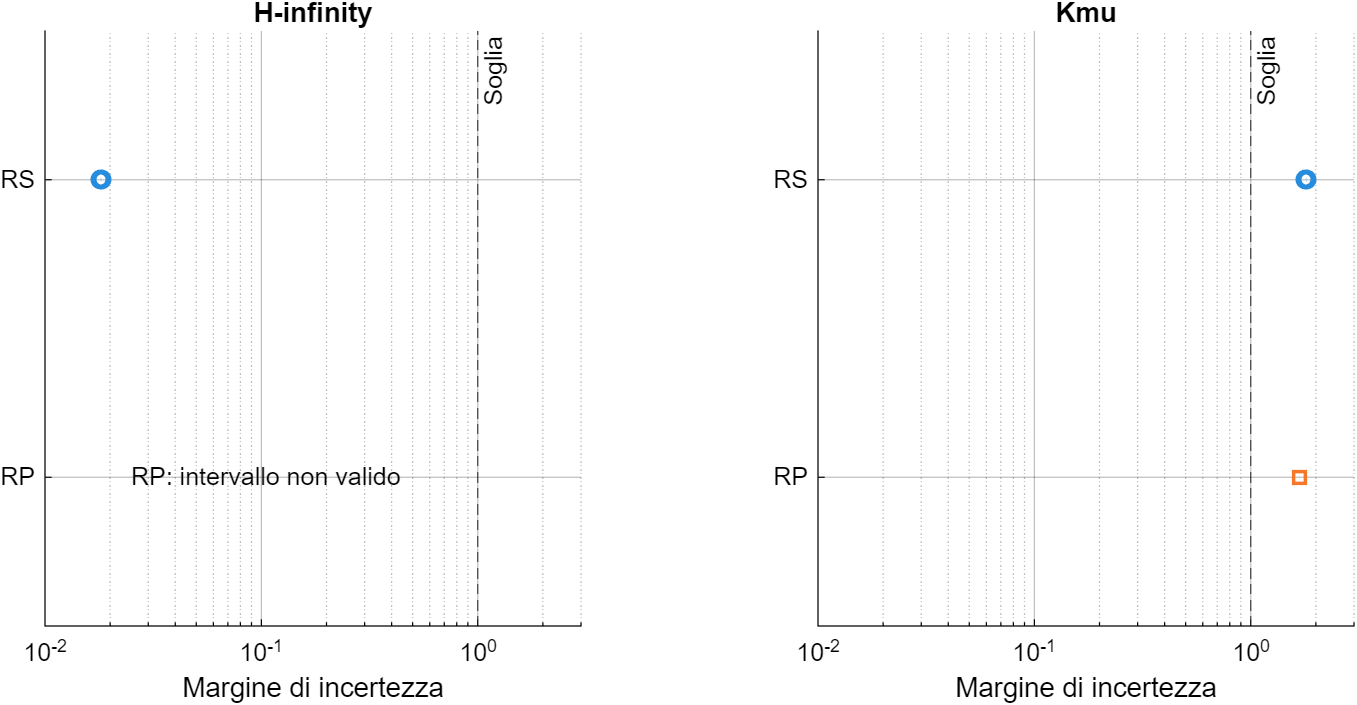
\includegraphics[width=.94\textwidth]{figures/mu/robust_margins.png}
\caption{Margini rispetto alla soglia uno. L'intervallo RP non
valido del controllore nominale non è disegnato come garanzia.}
\end{figure}
Per $K_\mu$ i limiti inferiori RS e RP superano uno: il controllore
soddisfa NS, NP, RS e RP per il modello lineare incerto dichiarato.
La norma nominale \FinalMuGamma\ è peggiore di quella del comparatore
$H_\infty$, ma la proprietà è mantenuta sull'intero dominio modellato.
Il prezzo è l'ordine 78 e un tracking ancora oltre il target:
$T_s=1.522,1.478$ s; sul primo giunto l'errore statico è circa 6\%,
sopra il 5\% richiesto. RP e requisiti temporali sono distinti.

Il campionamento comune conferma empiricamente la differenza:
$H_\infty$ è stabile in 0/40 impianti, $K_\mu$ in 40/40.
I 120 attuatori dell'inviluppo e questi 40 impianti chiusi sono
insiemi usati per scopi diversi. La Monte Carlo non sostituisce
 i margini e non ne dà un'interpretazione probabilistica.
Il dettaglio dei campioni è nel Capitolo 11; le verifiche
non lineari e di rumore nel Capitolo 10 non estendono RS/RP
all'hardware o a fenomeni esclusi dal modello.

\section{Riferimenti per i comandi MATLAB}
Le convenzioni sono documentate da MathWorks per
\href{https://www.mathworks.com/help/robust/ref/inputoutputmodel.lftdata.html}{\texttt{lftdata}},
\href{https://www.mathworks.com/help/robust/ref/dynamicsystem.robstab.html}{\texttt{robstab}},
\href{https://www.mathworks.com/help/robust/ref/dynamicsystem.robgain.html}{\texttt{robgain}}
 e \href{https://www.mathworks.com/help/robust/ug/d-k-iteration-process.html}{iterazione D--K}.
Strutture, numeri e conclusioni derivano dai dati del nostro
repository, tracciati nelle appendici.

\chapter{Validazione non lineare nominale}
\section{Equazioni e scenari}
La campagna integra direttamente in MATLAB le equazioni SEA con i
parametri, gli attuatori e l'equilibrio descritti nei capitoli iniziali. La legge implementata è
\[
 \delta u=C_Kx_K+D_K[r;\delta q],\qquad
 \dot x_K=A_Kx_K+B_K[r;\delta q],\qquad u=\bar\tau+\delta u.
\]
Si usa \texttt{ode23t}, con tolleranze relativa $10^{-5}$ e assoluta $10^{-7}$,
passo massimo 0.005 s e uscita ogni 0.002 s. Queste prove usano MATLAB, non Simulink. Il confronto locale con la mappa
lineare è verificato automaticamente per entrambi i controllori.

Gli scenari conservano gradini di 2, 5 e 8 gradi su ciascun giunto (4 s),
disturbi lato link di 0.25, 0.5 e 1 N m (8 s), equilibrio e rumore (4 s).
L'errore statico non lineare è stimato dalla media dell'ultimo 10\% della
traiettoria. È una stima a orizzonte finito, da leggere insieme
all'assestamento; il guadagno DC lineare è una quantità distinta.

\section{Tracking, disturbi e rumore}
Gli equilibri restano invariati entro $1.7\,10^{-12}$ rad per H-infinity e
$2.3\,10^{-15}$ rad per Kmu. I gradini confermano l'assenza di overshoot
nei due controllori. Per $K_\mu$ a 5 gradi si misurano $T_s=1.522,1.484$ s,
errori relativi circa 6.03\%, 3.08\% e picchi di comando 0.796,0.199 N m.
I risultati conservano i fallimenti delle specifiche temporali di assestamento e, per Kmu sul primo
giunto, offset. Risposte e metriche di tutti i disturbi fisici sono salvate
con il controllore che le ha prodotte.

Il rumore usa esattamente due canali della sequenza encoder salvata,
con seed 20260826. La ripetizione restituisce differenza nulla.
Qui emerge un limite decisivo del candidato H-infinity: il picco di comando
è circa 5685 N m, con RMS 118.2 N m. Per Kmu si ottengono circa 8.12 N m
e 1.934 N m. Il piccolo comando nel tracking privo di rumore non descrive
dunque la sensibilità del controllore H-infinity alle misure disturbate.
Non si aggiunge una saturazione numerica per nascondere questo risultato.

\section{Regione di attrazione empirica}
La sezione iniziale conserva $\delta\theta=\delta q$, velocità nulle,
attuatori all'equilibrio e stato del controllore nullo. Restano la griglia
$\{-60,-30,0,30,60\}^2$ gradi, 36 direzioni, precisione radiale di un grado,
orizzonti 8/12 s e i criteri dichiarati nel protocollo RAS. Il superamento del limite numerico
originario $10^6$ termina anticipatamente la simulazione: quel punto avrebbe
comunque fallito il criterio di limitatezza. Le metriche di coda sono valutate
sull'uscita uniforme MATLAB. Le sezioni confrontano i due controllori robusti sullo stesso
protocollo MATLAB; non sono una RAS dei modelli Simulink originali.

Per H-infinity convergono 27 dei 285 punti esaminati; il raggio minimo risolto
è zero e il massimo circa 6.98 gradi. Zero significa che la ricerca a
risoluzione di un grado non individua un punto convergente in alcune direzioni,
non che un sistema localmente stabile abbia regione di attrazione vuota.
Per Kmu convergono tutti i 57 punti e tutti gli estremi radiali del box.
La regione è quindi limitata dal dominio esplorato, non da una frontiera
fisica identificata. Il comando massimo tra i casi convergenti raggiunge
circa 61.1 N m per H-infinity e 2763 N m per Kmu: queste regioni senza
saturazione non sono regioni operative certificate dell'hardware.
\begin{figure}[htbp]\centering
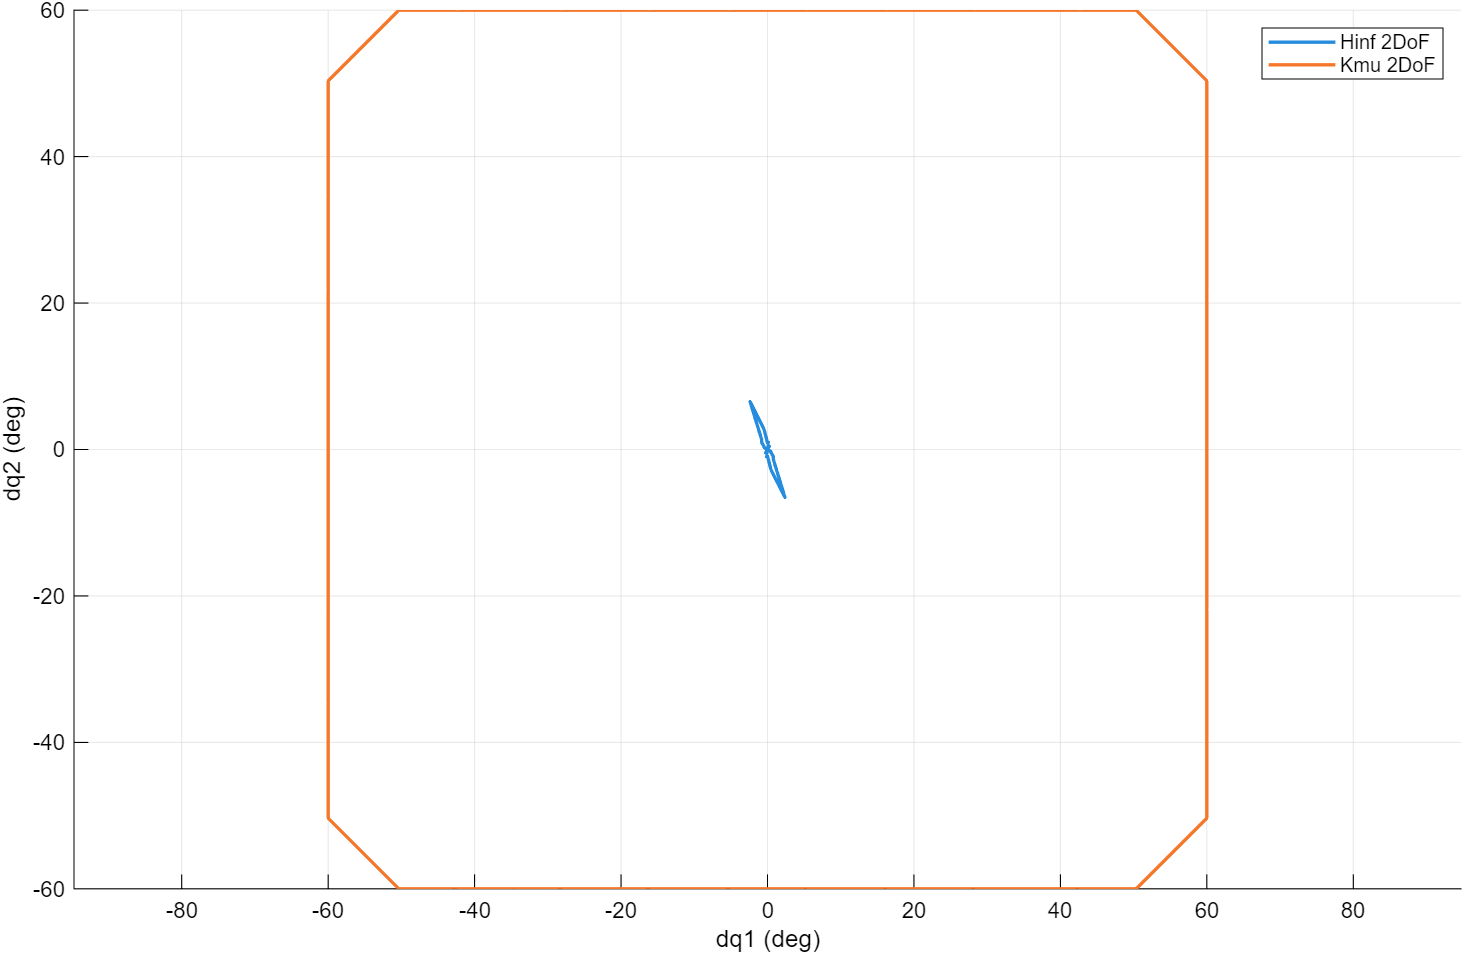
\includegraphics[width=.7\textwidth]{figures/hinf_final/ras.png}
\caption{Sezioni empiriche nominali con gli stessi criteri di convergenza.}
\end{figure}

\section{Verifica Lyapunov}
Si include l'intero stato aumentato e si risolve
$A_{cl}^TP+PA_{cl}=-I$. Per H-infinity il residuo è circa 65.27:
il controllo numerico fallisce e non si accredita alcun certificato.
Per Kmu, con 92 stati complessivi, $P$ è positiva e il residuo è 0.04493,
inferiore alla soglia preesistente 0.1. La stessa maggiorazione cubica del
resto SEA fornisce $\rho_{\mathrm{interno}}\simeq1.066\,10^{-12}$.
Il livello circa 3.697 supera la verifica su 2048 direzioni indipendenti
alle quattro frazioni radiali dichiarate; è evidenza su punti finiti,
non un'estensione del certificato analitico. Il risultato non viene trasferito a LQG o LQRI.

\section{Implementazioni MATLAB/Simulink adottate}\label{sec:originali}
Il progetto comprende otto modelli degli studenti: una coppia lineare e
non lineare per LQG, LQGI, $H_\infty$ e $\mu$-sintesi. Le copie originali
sono identificate da un manifest SHA-256. I modelli lineari usano 14 stati
fisici, quattro uscite encoder e otto ingressi nell'ordine
$[u;d;w_{link};w_u]$. Le misure rumorose alimentano il controllore,
mentre i rumori di processo sono applicati alla pianta.

LQG realizza $u=N_rr-K\hat x$ con un filtro di Kalman a 14 stati. LQGI
mantiene lo stesso osservatore e aggiunge due integratori sull'errore
misurato, $\dot\xi=r-q_{mis}$, con $u=-K_x\hat x-K_i\xi$.
Il modello $H_\infty$ confronta tre rami: il controllore 1-DoF riceve
$r-q_{mis}$, mentre 2-DoF e PID ricevono $[r;q_{mis}]$. Il modello
$\mu$ usa $K_\mu$ con la stessa interfaccia a quattro ingressi.
Le matrici dei rami 2-DoF condividono gli stati tra riferimento e misura.

I modelli non lineari integrano gli otto stati meccanici assoluti,
calcolano il disturbo sulle accelerazioni dei link e aggiungono i due
attuatori LTI. Le misure sono riportate in deviazioni dall'equilibrio
prima di essere usate dal controllore. L'inizializzazione esterna
\path{setup_student_originals.m} restituisce tutte le matrici e i tipi
Workspace necessari senza cambiare parametri o collegamenti interni.

L'ispezione ZIP/XML verifica segni, interfacce e varianze nei limiti di
un controllo statico. Tutti gli otto file sono R2026a Update 4; i tentativi
di caricamento con R2025b Update 4 falliscono per incompatibilità di
release. Nessuna simulazione o esportazione grafica nuova degli SLX è
accreditata. Per le figure e i dati Simulink sono predisposti comandi di
validazione nella release corretta; i grafici di questo capitolo sono
identificati esplicitamente come risultati MATLAB.


\chapter{Verifica pratica della robustezza su impianti incerti}

\section{Dieci impianti fisici comuni}
Per osservare come cambiano le prestazioni, estraiamo una volta
dieci quintuple di parametri con seed 20261101. La frequenza
naturale di ciascun drive cambia la zona in cui il comando è
attenuato, il ritardo ne cambia la fase e la massa $m_2$ modifica
la dinamica meccanica. Le frequenze sono fra 34 e 46 rad/s, i
ritardi fra 12 e 18 ms e la massa fra 0.72 e 0.88 kg. Lo
smorzamento dei drive resta a 0.8. Tutti i controllori sono
confrontati sulle stesse dieci quintuple e sul nominale, così
un caso sfavorevole può essere ripetuto con un altro controllore
senza cambiare la pianta. I valori sono salvati in
\texttt{parametri\_dieci\_impianti.csv}.
\begin{table}[htbp]\centering\small
\setlength{\tabcolsep}{4pt}
\begin{tabular}{lrrrrr}\toprule
Impianto & $\omega_{n1}$ & $\omega_{n2}$ & $\tau_{d1}$ & $\tau_{d2}$ & $m_2$\\\midrule
1 & \num{40.86} & \num{39.09} & \num{15.03} & \num{12.08} & \num{0.7793}\\
2 & \num{44.11} & \num{42.51} & \num{17.78} & \num{17.49} & \num{0.7559}\\
3 & \num{39.15} & \num{35.1} & \num{16.16} & \num{17.09} & \num{0.8014}\\
4 & \num{35.72} & \num{38.63} & \num{14.81} & \num{12.49} & \num{0.8038}\\
5 & \num{41.49} & \num{42.74} & \num{15.19} & \num{17.38} & \num{0.8181}\\
6 & \num{42.38} & \num{45.67} & \num{14.26} & \num{15.62} & \num{0.7903}\\
7 & \num{45.66} & \num{38.28} & \num{14.66} & \num{14.52} & \num{0.8205}\\
8 & \num{44.33} & \num{43.17} & \num{16.33} & \num{13.77} & \num{0.845}\\
9 & \num{45.23} & \num{41.22} & \num{14.36} & \num{13.02} & \num{0.7454}\\
10 & \num{44.54} & \num{34.26} & \num{14.49} & \num{17.23} & \num{0.8613}\\
\bottomrule\end{tabular}
\caption{Dieci impianti fisici comuni, seed 20261101. Frequenze in rad/s, ritardi in ms e massa in kg; smorzamento 0.8 noto.}
\end{table}


\section{Le rappresentazioni A e B sugli stessi campioni}
In A le frequenze, i ritardi e la massa entrano direttamente
come parametri fisici. In B il drive nominale riceve una
correzione dinamica additiva: il peso $W_A$ scala lo
scostamento possibile con la frequenza e una perturbazione
normalizzata ne specifica la dinamica. La massa $m_2$ resta
un parametro meccanico in entrambe.

Per ciascuno dei dieci impianti la perturbazione additiva
che ricostruisce il drive è la differenza rispetto al nominale
divisa per $W_A$. È stata controllata per stabilità, proprietà
e norma. Il massimo errore relativo di ricostruzione A/B è
\FinErroreAB. A controllore fissato le risposte dei due modelli
allo stesso campione coincidono entro questa precisione di
rappresentazione. B ammette anche dinamiche senza una
corrispondente coppia fisica di frequenza e ritardo, e la
copertura dell'intero box A resta da dimostrare. Il confronto
dei margini del Capitolo 9 valuta l'effetto di queste differenze
sull'intera famiglia dichiarata.

\section{Stabilità interna e tracking}
Prima di misurare il tracking si controllano tutti i poli
della chiusura. Un polo con parte reale positiva fa crescere
un modo interno, anche quando l'uscita di una certa prova
lo mostra poco. I casi instabili restano nel conteggio
(Tabella~\ref{tab:impianti-comuni}); i massimi di errore e
comando usano soltanto i casi stabili.

\begin{table}[htbp]\centering\small
\setlength{\tabcolsep}{4pt}
\begin{tabular}{lrrrr}\toprule
Controllore & Stabili & Errore DC [\%] & Picco u [N m] & Picco $q_d$ [$^\circ$]\\\midrule
LQG & 10/10 & \num{6.763} & \num{4.832} & \num{9.218}\\
LQGI & 10/10 & 0 & \num{0.9876} & \num{7.584}\\
Hinf1 & 10/10 & \num{15.54} & \num{14.74} & \num{14.63}\\
Hinf2 & 4/10 & \num{0.1643} & \num{1.001} & \num{2.717}\\
PID & 7/10 & 0 & \num{3.946} & \num{12.54}\\
Mu\_A & 10/10 & \num{99.8} & \num{0.001168} & \num{7.992}\\
Mu\_B & 10/10 & \num{22.36} & \num{0.8511} & \num{8.136}\\
\bottomrule\end{tabular}
\caption{Dieci impianti comuni: massimi sui soli casi stabili. Errore DC relativo e coppia link di 0.5 N m.}
\end{table}


Hinf2 resta stabile in \FinHinfTwoStable/10 campioni e PID in
\FinPIDStable/10. Il basso errore DC riportato per Hinf2
riguarda quindi un solo impianto incerto stabile. LQG, LQGI,
Hinf1, Mu\_A e Mu\_B sono stabili in tutti e dieci.
LQGI conserva un errore DC praticamente nullo nei campioni,
mentre il massimo di LQG sale al 5.41\%. La precisione statica
dei finali D--K è inferiore in questi casi, pur con tutti i
campioni stabili.

La Figura~\ref{fig:dieci-impianti} mostra quanto si allargano
i transitori al variare della pianta. Le metriche usano prove
con gradini separati sui due giunti. Si leggono assestamento
rispetto al valore finale, sovraelongazione rispetto al gradino,
errore statico rispetto al riferimento e cross-coupling,
ossia il picco del giunto non comandato diviso per i $5^\circ$
richiesti al giunto comandato. Mu\_A, per esempio, sposta
poco il secondo giunto ma manca il riferimento anche nel
nominale. La Tabella~\ref{tab:quattro-target} riporta il nominale
separatamente dai dieci campioni.

\begin{table}[htbp]\centering\small
\setlength{\tabcolsep}{4pt}
\begin{tabular}{lrrrrr}\toprule
Controllore & $T_s$ [s] & $M_p$ [\%] & $e_{ss}$ [\%] & Cross [\%] & Target\\\midrule
LQG & \num{0.731} & \num{0.346} & 0 & \num{18.4} & PASS\\
LQGI & \num{5.15} & \num{0} & 0 & \num{4.24} & FAIL\\
Hinf1 & \num{1.55} & \num{136} & \num{14.9} & \num{44.8} & FAIL\\
Hinf2 & \num{1.94} & \num{0} & \num{0.111} & \num{0.883} & PASS\\
PID & \num{5} & \num{4.74} & 0 & \num{34.5} & FAIL\\
Mu\_A & $\infty$ & \num{0} & \num{99.8} & \num{0.0185} & FAIL\\
Mu\_B & \num{4.39} & \num{0} & \num{21.9} & \num{3.98} & FAIL\\
\bottomrule\end{tabular}
\caption{Nominale con carico: target simultanei 2 s, 15\%, 5\%, 25\%. Il tempo di assestamento è misurato rispetto al valore finale, l'errore DC rispetto al riferimento.}
\end{table}


\begin{figure}[!tbp]\centering
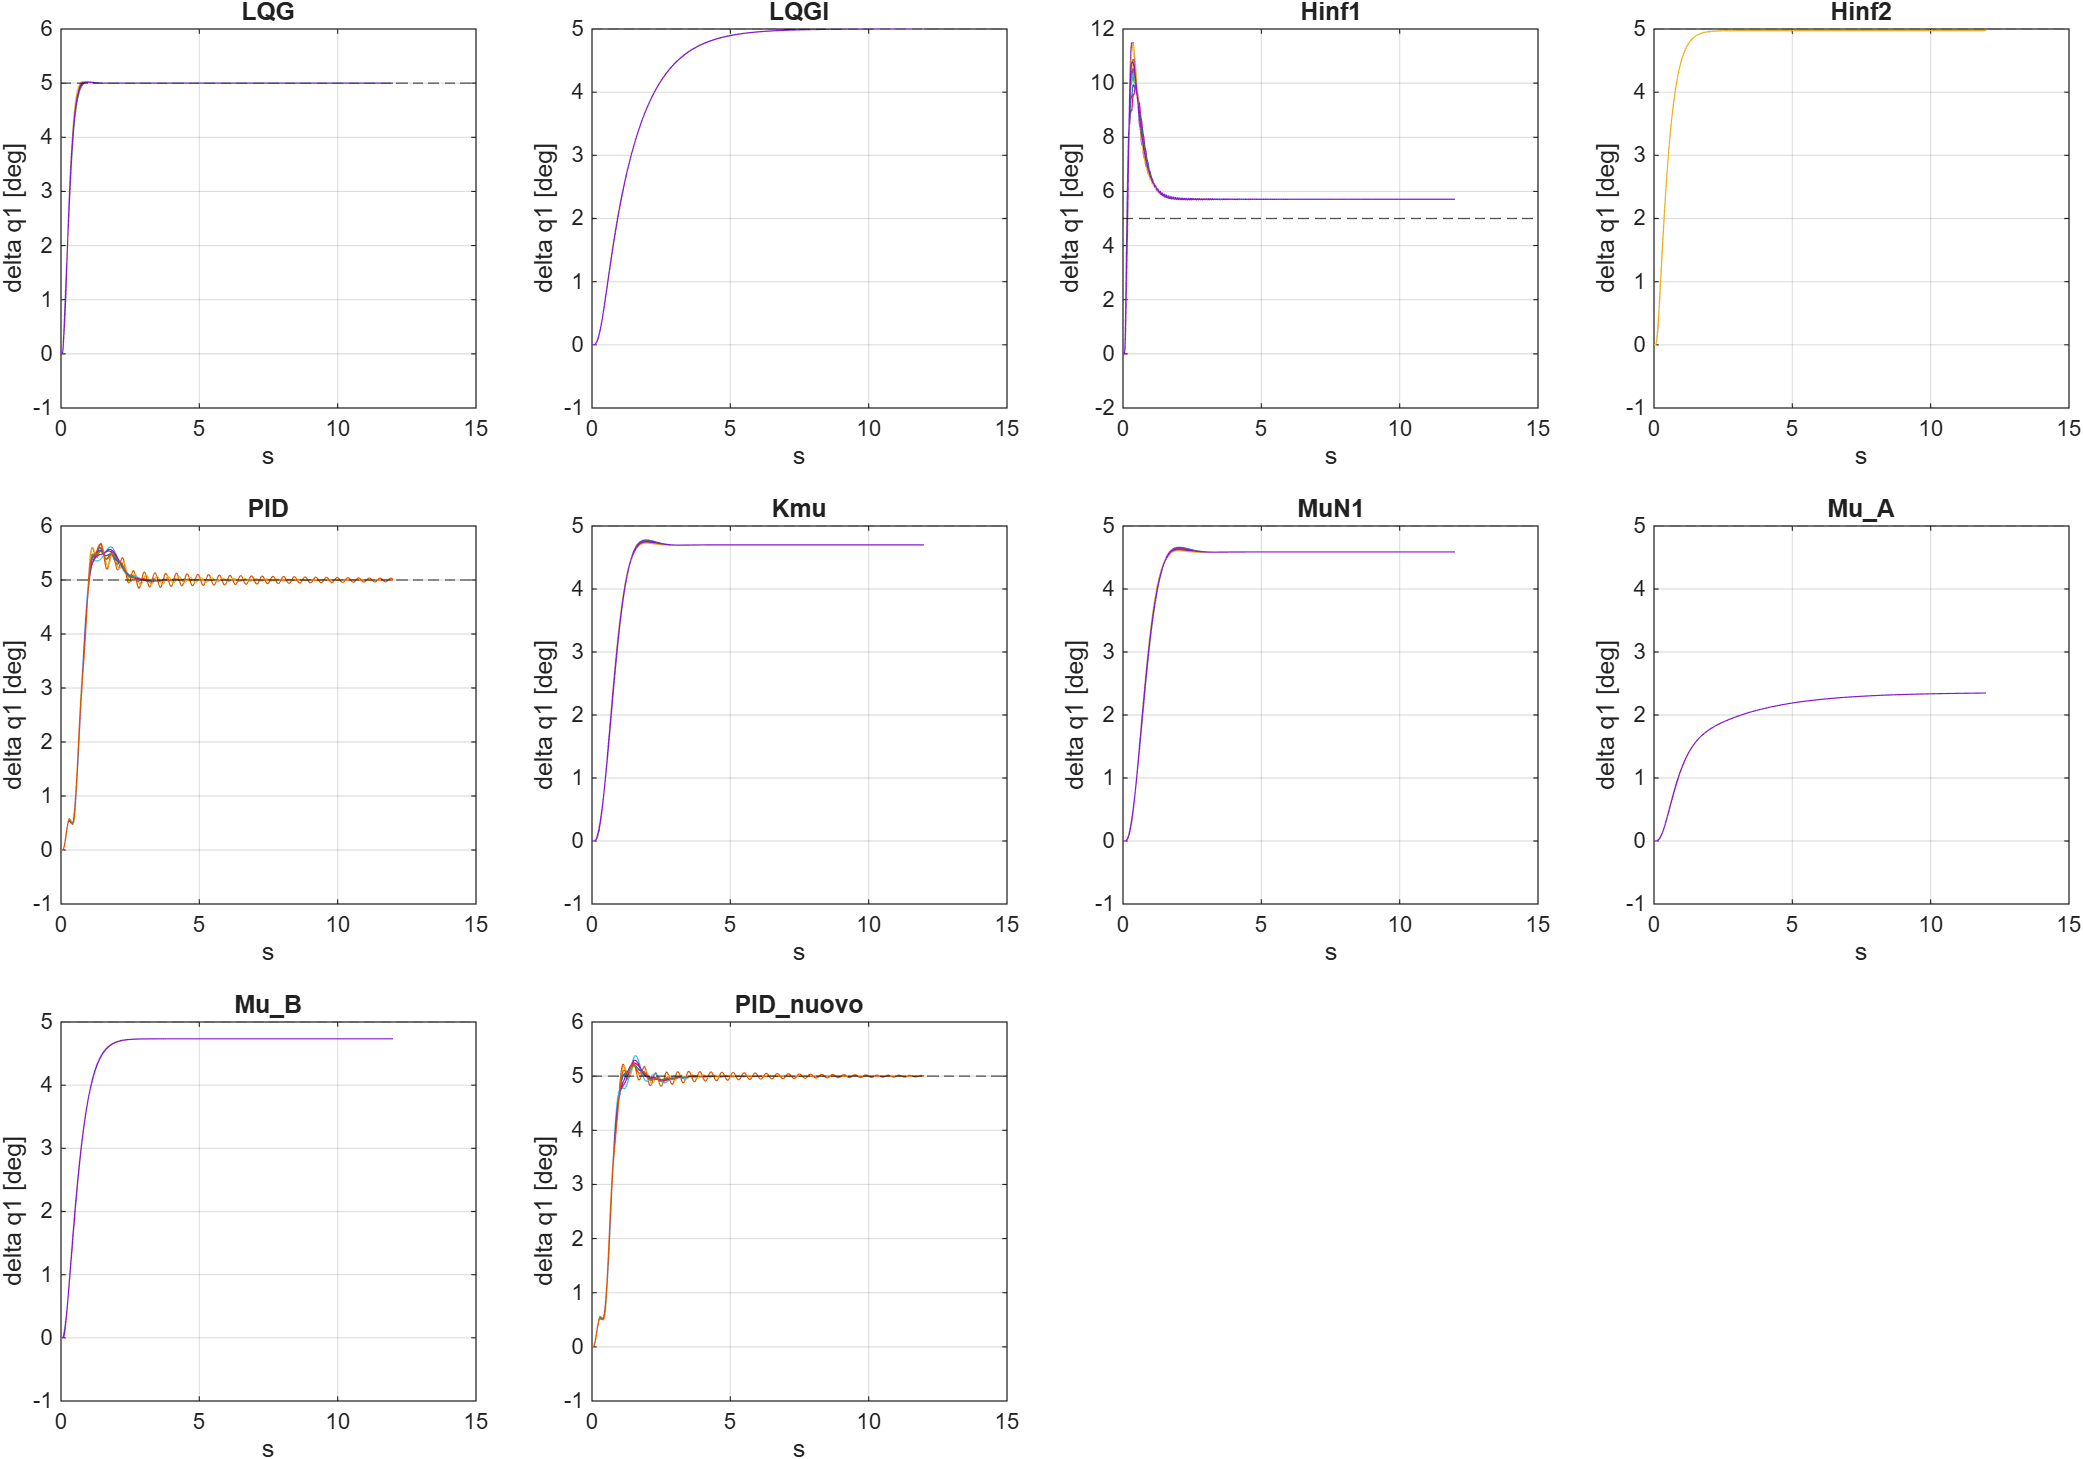
\includegraphics[width=.95\linewidth,height=.34\textheight,keepaspectratio]{figures/definitiva/dieci_impianti.png}
\caption{Gradino di $5^\circ$ al primo giunto. Le curve mostrano
il nominale e i campioni stabili. Il numero di curve di Hinf2 è
ridotto per via delle instabilità registrate in tabella.}
\label{fig:dieci-impianti}
\end{figure}

\section{Rigetto di coppia sui campioni stabili}
Con riferimento nullo applichiamo 0.5 N\,m a un link alla volta.
Il tempo di recupero misura il rientro di entrambi i giunti entro
$0.5^\circ$ dall'equilibrio per il resto della prova. In tabella,
$\infty$ indica rientro mancato entro l'orizzonte di 12 s.

\begin{table}[htbp]\centering\small
\setlength{\tabcolsep}{4pt}
\begin{tabular}{lrrr}\toprule
Controllore & Picco $q_d$ [$^\circ$] & Recupero nom. [s] & Recupero max [s]\\\midrule
LQG & \num{8.84} & $\infty$ & $\infty$\\
LQGI & \num{7.27} & \num{3.48} & \num{3.562}\\
Hinf1 & \num{14.3} & $\infty$ & $\infty$\\
Hinf2 & \num{2.1} & \num{0.346} & \num{0.658}\\
PID & \num{12} & \num{2.95} & \num{3.08}\\
Mu\_A & \num{6.12} & $\infty$ & $\infty$\\
Mu\_B & \num{6.8} & $\infty$ & $\infty$\\
\bottomrule\end{tabular}
\caption{Coppie link separate: peggiore asse nominale e massimo fra campioni stabili. Infinito indica mancato rientro entro 0.5 gradi nell'orizzonte di 12 s.}
\end{table}


Nel peggiore dei dieci casi LQGI rientra in circa 3.56 s,
mentre LQG manca il rientro già nel nominale. Hinf2
rientra in meno di un secondo nell'unico campione stabile.
Il picco di posizione e lo sforzo di comando completano
la lettura dei tempi di recupero.

\paragraph*{Portata della verifica.}
Dieci successi sono un riscontro empirico, mentre anche un solo
campione instabile esclude la garanzia di stabilità su A.
La $\mu$-analysis valuta la famiglia lineare dichiarata, incluse
dinamiche di B senza un corrispondente drive fisico della campagna.
Per valutare insieme variazioni parametriche e rumore encoder
servirebbe una campagna abbinata.
\FloatBarrier

\chapter{Confronto finale e scelta per ruolo}
Il confronto non individua un controllore che soddisfi contemporaneamente ogni obiettivo. Le famiglie mettono in evidenza compromessi diversi, che diventano più chiari quando massa e ritardi variano insieme.

LQG stabilizza in modo robusto entrambe le rappresentazioni e limita bene il comando prodotto dal rumore. Il prefiltro offre precisione sul nominale, ma non corregge automaticamente l'offset dovuto a un carico diverso o a una coppia costante. È una soluzione utile per mostrare il ruolo dello stato stimato e il limite di un inseguimento senza integrazione.

LQGI aggiunge soltanto due stati e mantiene la stabilità robusta. L'integratore corregge l'errore misurato nei casi stabili e rende il tracking meno sensibile alla massa. Il prezzo osservato è il tempo di assestamento, che supera il target scelto. Per un compito di posizionamento lento e preciso è il candidato più comprensibile da approfondire, senza dichiararlo già conforme a tutte le specifiche.

Hinf1 mostra come la sensibilità mista controlli trasferimenti pesati senza garantire una buona forma del transitorio. Passare alla struttura 2-DoF permette a Hinf2 di seguire molto meglio il modello desiderato sul nominale. Tuttavia il suo margine robusto è piccolo e il rumore genera coppie molto elevate. La piccola norma nominale è quindi un risultato matematico corretto, ma insufficiente a motivarne l'uso.

Il PID strutturato contiene pochi stati e conserva una legge facilmente riconoscibile. Ottiene NP sul costo comune, ma non RS. La semplicità della struttura non elimina l'accoppiamento del braccio né il ritardo dei drive: i due canali diagonali hanno una libertà limitata per affrontarli.

La D--K incorpora direttamente la struttura incerta, ma il problema non è convesso e gli scaling aumentano l'ordine. Le due sintesi eseguite con uguali pesi e inizializzazione non raggiungono l'obiettivo robusto unitario. Mu\_A lascia un errore DC di circa il 99.8\%, mentre Mu\_B lascia circa il 21.9\% e amplifica il rumore fino a un picco osservato di circa 762 N m. Entrambi mantengono RS, ma queste prestazioni non ne motivano l’adozione. Il confronto rimane utile perché mostra quanto una descrizione più ricca o più libera possa cambiare la ricerca. Non scegliamo un candidato soltanto perché proviene da una sintesi robusta.

\section{Che cosa offre la rappresentazione parametrica}
A conserva il significato di ogni variazione. Una massa più grande modifica insieme inerzia e gravità; un ritardo più grande sposta insieme il polo e lo zero di Padé. Questa correlazione evita che l'analisi combini coefficienti fisicamente incompatibili. È la descrizione naturale quando gli intervalli dei parametri sono noti e il modello fisico è credibile.

Il costo è la complessità della struttura reale ripetuta: sette grandezze non significano sette sole porte. Prodotti, inversi e ripetizioni possono rendere più impegnative l'analisi e la sintesi. La fedeltà della famiglia non rende automaticamente semplice il calcolo.

\section{Che cosa offre la rappresentazione concentrata}
B riassume gli scostamenti dei drive in due perturbazioni dinamiche e un peso comune. Il procedimento SISO rende leggibile il passaggio dalla famiglia all'inviluppo e al fit. Il carico resta esplicito nella meccanica: il confronto riguarda davvero il modo di rappresentare gli attuatori.

Il prezzo è la libertà concessa a dinamiche che non corrispondono necessariamente a frequenze, smorzamenti e ritardi fisici della famiglia. Questa libertà può ridurre i margini dimostrabili. Inoltre il peso è verificato su un insieme finito di casi: la copertura globale resta un limite dichiarato.

Le due rappresentazioni sono quindi strumenti complementari. A aiuta a spiegare l'origine fisica delle variazioni; B offre una descrizione dinamica compatta dei drive coperti. Nei dieci impianti ricostruiti, a controllore fissato, producono la stessa risposta. Sono le garanzie sull'insieme ammesso a cambiare.

\chapter{Conclusioni e limiti}
Il progetto ha costruito una catena riproducibile dal modello non lineare ai controllori e alle verifiche nominali, non lineari, empiriche e formali. M6 offre il miglior tracking nominale fra i candidati finali, ma M16 osserva una perdita di stabilità nel Sample 5. $K_{\infty}$ e $K_\mu$ sono stabili sui 40 campioni M16; soltanto $K_\mu$ possiede la Robust Stability formalmente certificata su M4.

La conclusione positiva è circoscritta: $K_\mu$ non soddisfa Nominal Performance né Robust Performance e non raggiunge i target di tracking M5. M7 non produce un controllore LQG-I finale. Il risultato finale è quindi una selezione per ruolo e non una conformità complessiva.
\section{Limiti noti}
% Tabella generata da build_m18_report_tables.m.
\begin{itemize}
\item Nessun controllore principale soddisfa tutte le specifiche M5
\item Kmu possiede RS formale, ma fallisce NP e RP in M14
\item M6 e Khinf non dispongono di una certificazione RS formale su M4
\item M16 fornisce evidenza empirica lineare e non una certificazione di robustezza
\item Le RAS M8/M15 sono empiriche; i limiti del box non sono frontiere dinamiche
\item uScale=12 N m è una normalizzazione; non è dichiarata alcuna saturazione
\item Il limite interno di Lyapunov vale sul nominale aumentato; il livello piu ampio campionato non e certificato
\item La maggiorazione e conservativa e valutata in double, senza aritmetica intervallare
\item Nessuna riduzione o nuova sintesi robusta nella revisione; sono aggiunte analisi nominali di Lyapunov e sensibilita Kalman
\end{itemize}

Mancano limiti hardware di coppia verificati e un modello di saturazione; i range M4 non sono identificati sperimentalmente; le RAS M8/M15 sono stime empiriche; la Monte Carlo non è un certificato; $K_\mu$ resta di ordine 52. Questi elementi non sono stati chiusi artificialmente in M18.
\section{Sviluppi futuri}
Sviluppi plausibili, non eseguiti, includono identificazione sperimentale delle incertezze, definizione dei limiti di attuazione, revisione motivata dei pesi, riduzione di $K_\mu$ con rivalidazione, architetture 2-DoF e validazione non lineare incerta. Ognuno richiederebbe una nuova fase tecnica e non cambia gli esiti qui documentati.

\appendix
\chapter{Parametri principali}\label{app:parametri}
% Generated by build_m18_report_tables.m. Do not edit.
\begin{table}[H]
\centering
\begin{tabular}{lll}
\toprule
Parametro & Valore & Unita \\
\midrule
$m_1$ & 1 & kg \\
$m_2$ & 0.8 & kg \\
$l_1$ & 0.4 & m \\
$l_2$ & 0.3 & m \\
$J_{m1}=J_{m2}$ & 0.01 & kg m$^2$ \\
$B_{m1}=B_{m2}$ & 0.02 & N m s/rad \\
$k_1$ & 50 & N m/rad \\
$k_2$ & 40 & N m/rad \\
$g$ & 9.81 & m/s$^2$ \\
\bottomrule
\end{tabular}
\caption{Parametri nominali principali.}
\label{tab:nominal-parameters}
\end{table}

I valori provengono da \artifact{sea\_params\_nominal.m} e dai dataset di equilibrio e modello completo. La tabella non introduce metadata di laboratorio o tolleranze non presenti nel progetto.

\chapter{Tracciabilità dei risultati}
La catena corrente H-infinity è raccolta in
\path{results/data/hinf_final_coherent/}. La relazione legge le quantità
esportate da MATLAB con \path{export_hinf_final_results.m}; il successivo
\path{report/build_hinf_final_text.py} formatta testo e tabelle senza
calcolare controllori, norme, poli o metriche di controllo.

\begin{longtable}{p{.40\textwidth}p{.52\textwidth}}\toprule
Dataset corrente & Evidenza\\\midrule
\path{nominal_study.mat} & 21 profili 1-DoF e tre veri problemi 2-DoF\\
\path{selected_full_order.mat} & Identità del comparatore H-infinity\\
\path{fixed_study.mat} & 66 avvii con obiettivi e verifiche indipendenti\\
\path{m12.mat} & N--Delta e margini del comparatore selezionato\\
\path{m13.mat}, \path{m14.mat} & D--K corrente e post-analisi indipendente\\
\path{nonlinear_study.mat}, \path{noise_study.mat} & Equilibrio, gradini, disturbi e rumore\\
\path{ras_study.mat}, \path{lyapunov_study.mat} & Sezioni empiriche e verifica nominale\\
\path{monte_carlo_study.mat} & Sequenza paired e nuove chiusure\\
\path{summary.json} & Esportazione delle quantità per M17/M18\\
\path{hinf_final_traceability.json} & Provenienza delle macro della relazione\\\bottomrule
\end{longtable}
I file dati anteriori rimangono nei percorsi originali. Testo e PDF
precedenti sono inoltre conservati in \path{report/archive/before_final_coherent/}.
Le prime prove con tolleranza solver predefinita sono conservate nella
sottodirectory \path{numerical_diagnostics_default_solver/}; non costituiscono
la selezione corrente. M0--M8 e i relativi sorgenti della relazione restano
congelati. Le macro storiche necessarie a quei capitoli non sono usate per
presentare come attuali risultati dei vecchi controllori robusti.
Il resoconto di revisione raccoglie errori numerici, test e limiti residui.

\chapter{Riproducibilità}
Dalla radice del repository, MATLAB R2025b esegue l'intera pipeline con:
\begin{verbatim}
run_all
\end{verbatim}
Il comando pulisce il workspace, imposta il seed, aggiunge i percorsi del progetto e percorre M1--M18. M13 ricarica il checkpoint D--K congelato senza nuova chiamata a \texttt{musyn}. La generazione M18 si ripete con:
\begin{verbatim}
validate_m18_deliverables(true,true)
\end{verbatim}
Relazione e presentazione sono compilate con:
\begin{verbatim}
powershell -ExecutionPolicy Bypass -File tools/build_m18_latex.ps1
\end{verbatim}
I PDF finali hanno nomi stabili; file aux, log, toc, cache e altri intermedi non sono tracciati.

\chapter{Principali codici MATLAB del progetto}\label{app:matlab}
Questa appendice raccoglie i passaggi necessari per leggere e riprodurre
il metodo, senza riportare plotting e salvataggi ripetitivi.
Ogni listato è incluso direttamente dal file indicato: non è una
riscrittura del codice. Gli estratti richiedono gli argomenti, i dati
e le funzioni del file completo; non sono script autonomi da incollare
ed eseguire in sequenza.

Per i Capitoli 8--9 la fonte corrente è la campagna
\path{analysis/run_hinf_final_*.m} e i dati in
\path{results/data/hinf_final_coherent}. Gli script didattici
\path{progetto_hinf.m} e i dataset M9--M14 nella radice di
\path{results/data} descrivono anche configurazioni precedenti:
non ne trasferiamo pesi, ordini e risultati alla campagna finale.
Le verifiche che non ripetono le sintesi sono nell'Appendice C.


\section{Parametri, equilibrio e linearizzazione}

\par\medskip\noindent\begin{minipage}{\textwidth}\textbf{File:} \path{src/parameters/sea_params_nominal.m}\par\noindent\textit{Scopo.} Definisce i parametri meccanici nominali centralizzati.

\lstinputlisting[firstline=6,lastline=13]{../src/parameters/sea_params_nominal.m}\end{minipage}

\par\medskip\noindent\begin{minipage}{\textwidth}\textbf{File:} \path{src/model/sea_static_equilibrium.m}\par\noindent\textit{Scopo.} Calcola posizione dei motori e coppia statica per la postura assegnata. Nel progetto si passa $\bar q=[\pi/2;0]$.

\lstinputlisting[firstline=10,lastline=13]{../src/model/sea_static_equilibrium.m}\end{minipage}

\par\medskip\noindent\begin{minipage}{\textwidth}\textbf{File:} \path{src/model/sea_linearize_static_equilibrium_analytic.m}\par\noindent\textit{Scopo.} Costruisce i blocchi del Jacobiano statico. La stessa funzione accetta parametri numerici o incerti, conservando le dipendenze delle equazioni SEA.

\lstinputlisting[firstline=18,lastline=38]{../src/model/sea_linearize_static_equilibrium_analytic.m}\end{minipage}

\section{Attuatori e modello nominale a 14 stati}

\par\medskip\noindent\begin{minipage}{\textwidth}\textbf{File:} \path{src/actuators/build_nominal_actuator.m}\par\noindent\textit{Scopo.} Combina il secondo ordine con il ritardo approssimato tramite Padé del primo ordine. I valori nominali sono 40 rad/s, 0.8 e 15 ms.

\lstinputlisting[firstline=11,lastline=21]{../src/actuators/build_nominal_actuator.m}\end{minipage}

\par\medskip\noindent\begin{minipage}{\textwidth}\textbf{File:} \path{src/model/build_m3_full_plant.m}\par\noindent\textit{Scopo.} Collega gli otto stati meccanici ai sei dei due attuatori. Mantiene le viste delle quattro posizioni misurate e delle sole due posizioni articolari.

\lstinputlisting[firstline=7,lastline=18]{../src/model/build_m3_full_plant.m}\end{minipage}

\section{Costruzione delle incertezze}

\par\medskip\noindent\begin{minipage}{\textwidth}\textbf{File:} \path{src/uncertainty/build_uncertain_mechanical_plant.m}\par\noindent\textit{Scopo.} Crea uno scalare reale soltanto per i parametri selezionati nella tabella centrale; gli altri restano nominali. La tabella corrente assegna il 10\% a $k_1,k_2,J_{m1}$.

\lstinputlisting[firstline=60,lastline=65]{../src/uncertainty/build_uncertain_mechanical_plant.m}\end{minipage}

\par\medskip\noindent\begin{minipage}{\textwidth}\textbf{File:} \path{src/uncertainty/build_m4_uncertain_plant.m}\par\noindent\textit{Scopo.} Inserisce le due incertezze dinamiche indipendenti tramite l'inviluppo $W_I$. Gli intervalli della famiglia attuativa sono condensati in questi blocchi.

\lstinputlisting[firstline=7,lastline=14]{../src/uncertainty/build_m4_uncertain_plant.m}\end{minipage}

\section{LQR, filtro di Kalman e controllore LQG}

\par\medskip\noindent\begin{minipage}{\textwidth}\textbf{File:} \path{controllers/lqg/search_lqr_weights_m6.m}\par\noindent\textit{Scopo.} Costruisce il costo del candidato, calcola il feedback LQR e il guadagno statico sul riferimento. La selezione finale deriva dalla ricerca e dalle verifiche M6, non dal solo frammento.

\lstinputlisting[firstline=56,lastline=65]{../controllers/lqg/search_lqr_weights_m6.m}\end{minipage}

\par\medskip\noindent\begin{minipage}{\textwidth}\textbf{File:} \path{controllers/lqg/design_kalman_m6.m}\par\noindent\textit{Scopo.} Calcola Kalman con disturbi lato link, errore del comando e quattro misure encoder. Le scale sono ipotesi progettuali, non dati sperimentali.

\lstinputlisting[firstline=15,lastline=24]{../controllers/lqg/design_kalman_m6.m}\end{minipage}

\par\medskip\noindent\begin{minipage}{\textwidth}\textbf{File:} \path{controllers/lqg/build_lqg_no_integrator.m}\par\noindent\textit{Scopo.} Combina feedback e osservatore nel controllore senza integratore. Gli ingressi sono due riferimenti e quattro misure.

\lstinputlisting[firstline=28,lastline=31]{../controllers/lqg/build_lqg_no_integrator.m}\end{minipage}

\section{LQRI con osservatore e integratore dell'errore}

\par\medskip\noindent\begin{minipage}{\textwidth}\textbf{File:} \path{analysis/progetto_lqri.m}\par\noindent\textit{Scopo.} Mostra il problema LQR aumentato, la verifica Riccati e la realizzazione a 16 stati con Kalman M6. Si carica il candidato salvato all'indice \texttt{illustrativeIndex}; non si usa lo stato vero nel controllo.

\lstinputlisting[firstline=17,lastline=34]{../analysis/progetto_lqri.m}\end{minipage}

\section{Pesi, sensibilità mista e sintesi 1-DoF}

\par\medskip\noindent\begin{minipage}{\textwidth}\textbf{File:} \path{controllers/hinf/hinf_revision_weights.m}\par\noindent\textit{Scopo.} Costruisce i pesi dai cinque parametri del profilo; \texttt{c.alpha=6}. Il profilo finale è $(2,0.15,3,0.003,80)$.

\lstinputlisting[firstline=3,lastline=5]{../controllers/hinf/hinf_revision_weights.m}\end{minipage}

\par\medskip\noindent\begin{minipage}{\textwidth}\textbf{File:} \path{analysis/run_hinf_final_nominal.m}\par\noindent\textit{Scopo.} Esegue le due sintesi 1-DoF sugli stessi pesi e scrive il controllore equivalente con ingressi separati $[r;q]$. Le verifiche successive confrontano mappe, norme e poli.

\lstinputlisting[firstline=27,lastline=30]{../analysis/run_hinf_final_nominal.m}\end{minipage}

\par\medskip\noindent\begin{minipage}{\textwidth}\textbf{File:} \path{controllers/hinf/hinf_revision_plant.m}\par\noindent\textit{Scopo.} Costruisce esplicitamente $P$ con errore $r-q$, due uscite pesate e due segnali per il controllore.

\lstinputlisting[firstline=3,lastline=10]{../controllers/hinf/hinf_revision_plant.m}\end{minipage}

\section{Pianta 2-DoF, modello desiderato e partizioni del controllore}

\par\medskip\noindent\begin{minipage}{\textwidth}\textbf{File:} \path{analysis/run_hinf_final_nominal.m}\par\noindent\textit{Scopo.} Definisce il modello di riferimento criticamente smorzato. I tre valori di frequenza provati sono 2, 3 e 4 rad/s.

\lstinputlisting[firstline=66,lastline=67]{../analysis/run_hinf_final_nominal.m}\end{minipage}

\par\medskip\noindent\begin{minipage}{\textwidth}\textbf{File:} \path{controllers/hinf/hinf_final_2dof_plant.m}\par\noindent\textit{Scopo.} Collega modello fisico, $M_o$, $W_e$ e $W_u$ con errore $q-q_m$. Espone $[r;d;u]$ in ingresso e $[z_e;z_u;r;q]$ in uscita.

\lstinputlisting[firstline=4,lastline=11]{../controllers/hinf/hinf_final_2dof_plant.m}\end{minipage}

\par\medskip\noindent\begin{minipage}{\textwidth}\textbf{File:} \path{analysis/run_hinf_final_nominal.m}\par\noindent\textit{Scopo.} Sintetizza il controllore con quattro ingressi e due comandi; riferimento e feedback sono progettati insieme.

\lstinputlisting[firstline=71,lastline=72]{../analysis/run_hinf_final_nominal.m}\end{minipage}

\par\medskip\noindent\begin{minipage}{\textwidth}\textbf{File:} \path{controllers/hinf/hinf_final_evaluate.m}\par\noindent\textit{Scopo.} Partiziona $B_K,D_K$ nei canali $r$ e $q$, mantenendo $A_K,C_K$ condivise. La matrice chiusa verifica il segno $u=K_rr+K_yq$ e la stabilità interna senza cancellazioni.

\lstinputlisting[firstline=3,lastline=9]{../controllers/hinf/hinf_final_evaluate.m}\end{minipage}

\section{Sintesi strutturata sullo stesso problema}

\par\medskip\noindent\begin{minipage}{\textwidth}\textbf{File:} \path{analysis/run_hinf_final_fixed.m}\par\noindent\textit{Scopo.} Definisce le famiglie statico, PI, PID e MIMO a ordine assegnato, con undici avvii e seed per famiglia. Le verifiche di ciascun risultato seguono nel file completo.

\lstinputlisting[firstline=15,lastline=27]{../analysis/run_hinf_final_fixed.m}\end{minipage}

\section{Pianta incerta, analisi e sintesi robusta correnti}

\par\medskip\noindent\begin{minipage}{\textwidth}\textbf{File:} \path{controllers/hinf/hinf_final_uncertain.m}\par\noindent\textit{Scopo.} Preserva le proprietà incerte della meccanica e l'oggetto dinamico degli attuatori, aggiungendo il disturbo fisico lato link. Usare solo le matrici nominali eliminerebbe parte delle incertezze.

\lstinputlisting[firstline=4,lastline=11]{../controllers/hinf/hinf_final_uncertain.m}\end{minipage}

\par\medskip\noindent\begin{minipage}{\textwidth}\textbf{File:} \path{analysis/run_hinf_final_robust.m}\par\noindent\textit{Scopo.} Prepara le opzioni della singola campagna D--K e chiama \texttt{musyn} con le stesse porte del 2-DoF nominale.

\lstinputlisting[firstline=23,lastline=30]{../analysis/run_hinf_final_robust.m}\end{minipage}

Le opzioni salvate sono: cinque iterazioni, \texttt{TargetPerf=0},
\texttt{TolPerf=0.01}, \texttt{MixedMU='on'}, \texttt{FullDG=[true true]},
\texttt{FitOrder=[5 2]}, griglia di 1201 frequenze da $10^{-3}$ a
$10^4$ rad/s, scaling automatico, regolarizzazione e limitazione
del guadagno attivi, \texttt{RandomStart=0}, \texttt{UseParallel=false},
\texttt{MinDecay=1e-7}, \texttt{MaxFrequency=Inf}, seed 20260918.
\texttt{FitOrder} limita il fit degli scaling, non l'ordine finale di $K$.


\par\medskip\noindent\begin{minipage}{\textwidth}\textbf{File:} \path{analysis/run_hinf_final_robust.m}\par\noindent\textit{Scopo.} A controllore fissato ricalcola nominale, struttura LFT e margini RS/RP sulla pianta originale. La funzione successiva conserva l'intervallo RP invertito e ne registra l'esito non validato.

\lstinputlisting[firstline=47,lastline=51]{../analysis/run_hinf_final_robust.m}\end{minipage}

\section{Calcolo diretto di mussv: procedura delle analisi precedenti}

\par\medskip\noindent\begin{minipage}{\textwidth}\textbf{File:} \path{analysis/robust/analyze_m12_manual_mu.m}\par\noindent\textit{Scopo.} Calcola i limiti di $\mu$ per il ritorno dell'incertezza su una griglia fissata. È una funzione delle analisi M12 precedenti, non la fonte dei margini finali di ordine 22 e 78. Un picco campionato non certifica da solo tutto l'asse delle frequenze.

\lstinputlisting[firstline=11,lastline=15]{../analysis/robust/analyze_m12_manual_mu.m}\end{minipage}

\section{Campioni comuni e verifica Monte Carlo}

\par\medskip\noindent\begin{minipage}{\textwidth}\textbf{File:} \path{analysis/monte_carlo/generate_m16_uncertainty_samples.m}\par\noindent\textit{Scopo.} Genera la sequenza riproducibile M16, con seed 20260826 e 40 campioni. Lo stato del generatore è preservato; il file completo controlla range, norme e replay.

\lstinputlisting[firstline=9,lastline=12]{../analysis/monte_carlo/generate_m16_uncertainty_samples.m}\end{minipage}

\par\medskip\noindent\begin{minipage}{\textwidth}\textbf{File:} \path{analysis/run_hinf_final_monte_carlo.m}\par\noindent\textit{Scopo.} Ricarica e verifica i campioni comuni prima di valutarli con i controllori finali. Le configurazioni dei vecchi controllori nel file M16 non sono adottate come ordini dei nuovi controllori.

\lstinputlisting[firstline=11,lastline=13]{../analysis/run_hinf_final_monte_carlo.m}\end{minipage}

\section{Dinamica non lineare e collegamento con il controllore}

\par\medskip\noindent\begin{minipage}{\textwidth}\textbf{File:} \path{src/model/sea_nonlinear_rhs_with_link_disturbance.m}\par\noindent\textit{Scopo.} Valuta le otto equazioni meccaniche con coppia motore e disturbo positivo sulle accelerazioni dei link. Il caso senza disturbo è in \path{sea_nonlinear_rhs.m}.

\lstinputlisting[firstline=16,lastline=27]{../src/model/sea_nonlinear_rhs_with_link_disturbance.m}\end{minipage}

\par\medskip\noindent\begin{minipage}{\textwidth}\textbf{File:} \path{analysis/nonlinear/simulate_hinf_final_nonlinear.m}\par\noindent\textit{Scopo.} Collega gli otto stati SEA, i sei stati attuativi e lo stato condiviso di $K$. Le posizioni misurate sono incrementali e possono contenere il rumore salvato; il simulatore usa \texttt{ode23t}.

\lstinputlisting[firstline=34,lastline=39]{../analysis/nonlinear/simulate_hinf_final_nonlinear.m}\end{minipage}

La RAS nominale è calcolata da
\path{analysis/run_hinf_final_ras.m}, che richiama
\path{analysis/ras/estimate_m15_robust_ras.m} con lo stesso simulatore,
box, risoluzione e criteri del protocollo dichiarato. La chiamata
usa i controllori salvati e produce una sezione empirica, non
una certificazione globale. I risultati di questa relazione
non richiedono nuove ricerche RAS per essere letti o verificati.


\section{Formule di connessione e diagnosi del limite inferiore}

Le due LFT usate nei capitoli hanno le forme
\begin{equation}\label{eq:lowerlft}
 F_l(P,K)=P_{11}+P_{12}K(I-P_{22}K)^{-1}P_{21},
\end{equation}
\begin{equation}\label{eq:upperlft}
 F_u(N,\Delta)=N_{22}+N_{21}\Delta(I-N_{11}\Delta)^{-1}N_{12}.
\end{equation}
La prima chiude $u=Ky_K$ sulle porte inferiori; la seconda chiude
$w_\Delta=\Delta v_\Delta$ sulle porte superiori.
Nel codice \texttt{lft(Delta,M)} ricostruisce la seconda connessione.

Per la diagnosi 1-DoF, $S+GKS=I$ e $X=KS$.
A una frequenza fissata, con pesi scalari replicati
$a=|W_{1,s}|$, $b=|W_{2,s}|>0$, minimizzare
$a^2\|v-Gx\|^2+b^2\|x\|^2$ per una direzione unitaria $v$
fornisce il limite inferiore
\[
 \left\|\begin{bmatrix}W_1S\\W_2KS\end{bmatrix}\right\|_2
 \ge \frac{ab}{\sqrt{b^2+a^2\sigma_{\min}(G)^2}}.
\]
Si usa il valore singolare minimo, senza invertire $G$.
Il massimo sulla griglia è una diagnosi di richieste troppo severe:
non costruisce un controllore causale stabilizzante e non dimostra
la fattibilità quando è minore di uno. Il calcolo è in
\path{controllers/hinf/hinf_revision_lower_bound.m}, verificato
dai sette test in \path{tests/hinfLowerBoundTest.m}.

\end{document}
